\chapter{RESULTADOS E DISCUSSÃO}
% Version passo 0.005
% 'Sim ref'	'2.94'	49
% 'Sim 1A'	'2.95'	49
% 'Sim 1B'	'0.74'	49
% 'Sim 2A'	'5.43'	49
% 'Sim 2B'	'0.88'	49
% 'Sim 3A'	'4.30'	81
% 'Sim 3B'	'1.52'	45
% 'Sim 4A'	'0.22'	25
% 'Sim 4B'	'93.02'	241
% 'Sim 5A'	'4.98'	85
% 'Sim 5B'	'1.50'	37
Este capítulo detalha os resultados alcançados por meio da simulação computacional do método de controle de trajetória proposto pelo presente trabalho. É apresentado a sequência de movimentos a serem simulados, assim como os parâmetros da simulação. Além disso, são realizadas as simulações com variações dos valores destes parâmetros para uma análise da influência dos mesmos nos resultados. É utilizado também o algoritmo Runge-Kutta para simular a trajetória percorrida pela ponta da impressora dada a trajetória da base, fornecendo dados para se comparar a influência do método de controle de trajetória proposto.

\section{Simulação Computacional e Análise de Dados}

As simulações são realizadas a partir de dois movimentos lineares: um deslocamento de 10 milímetros no eixo x seguido de um movimento similar no eixo y, partindo da posição inicial (0,0) e em estado de repouso. A Figura \ref{fig:base_mov} ilustra estes movimentos.

\begin{figure}[H]
    \centering
    \caption{Movimento base}
    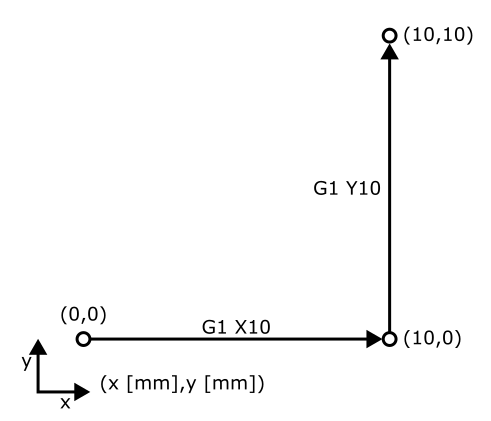
\includegraphics[scale=0.6]{base_mov}

    \label{fig:base_mov}
\end{figure}

Os parâmetros da simulação incluem a frequência natural e o coeficiente de amortecimento, responsáveis pela definição do modelo dinâmico da impressora. Adicionalmente, a aceleração e o passo de tempo são parâmetros que influenciam diretamente a trajetória, sendo estes definidos na fase de geração da mesma. Por fim, a velocidade estipulada no comando, que é parte integrante do Gcode, também é determinada. A origem e aplicação desses parâmetros são detalhadas na Figura \ref{fig:fluxo_geral_var}.

\begin{figure}[H]
    \centering
    \caption{Fluxograma geral com os parâmetros.}
    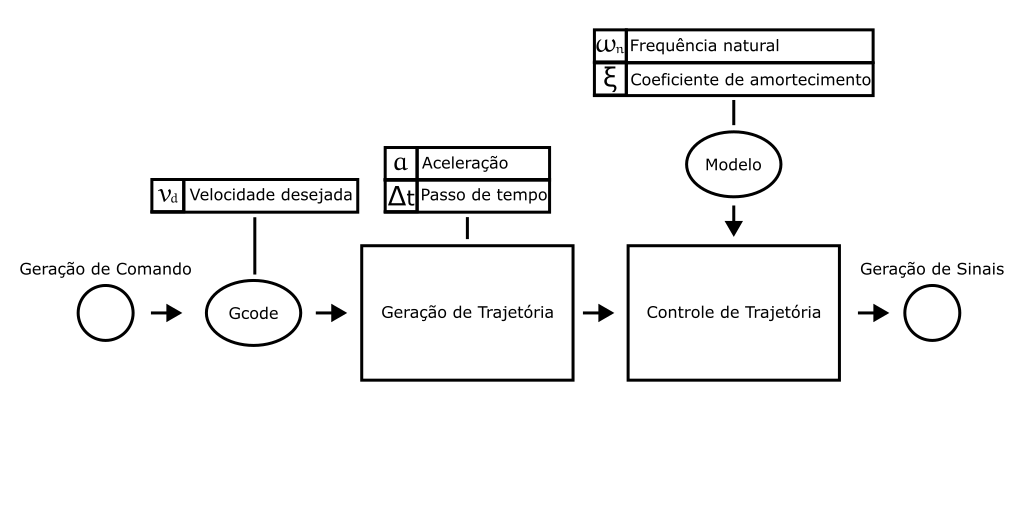
\includegraphics[scale=0.5]{fluxo_geral_var}

    \label{fig:fluxo_geral_var}
\end{figure}

As simulações foram executadas em um computador com as especificações listadas na Tabela \ref{tab:note_config}.

\begin{table}
    \begin{center}
    \caption{Especificações do computador}
    \label{tab:note_config}
    \begin{tabular}{c c}
        \hline
        Processador & Intel I7-5500U 2.40GHz \\
        Memoria & 8,00 GB \\
        Placa de vídeo & Nvidia Geforce 920M \\
        Sistema & 64 bits \\ \hline
    \end{tabular}
    \end{center}
\end{table}

\subsection{Simulação de Referência}
Nesta etapa, conduz-se uma simulação de referência empregando valores medianos dos parâmetros-chave. Esta simulação serve como base para avaliar o impacto de variações nos parâmetros em simulações subsequentes. Os valores referência utilizados são listados na Tabela \ref{tab:base_params}.

\begin{table}
    \begin{center}
    \caption{Valores dos parâmetros utilizados na simulação referência.}
    \label{tab:base_params}
    \begin{tabular}{c c c}
        Parâmetro & Valor & Unidade\\ \hline
        Frequência & 100 & $rad/s$\\
        Coeficiente de amortecimento & 0,5 & - \\
        Aceleração base & 5000 & $mm/s^2$ \\
        Velocidade desejada & 100 & $mm/s$ \\
        Passo de tempo & 0,005 & $s$ \\ \hline
    \end{tabular}
    \end{center}
\end{table}

\subsection{Simulações com Parâmetros Variados}
Para explorar o efeito de diferentes configurações, realizam-se simulações adicionais onde cada parâmetro - frequência natural, coeficiente de amortecimento, aceleração de entrada, velocidade desejada e  passo de tempo - é variado individualmente. Estas variações incluem valores tanto inferiores quanto superiores aos da simulação de referência. No total, são 11 simulações: 10 delas dedicadas a testar os limites inferiores e superiores de cada parâmetro e uma utilizando os valores de referência. Os detalhes de cada simulação, incluindo a identificação numérica e a letra indicativa do parâmetro modificado (A para inferiores, B para superiores), são apresentados na Tabela \ref{tab:sim_params}.

\begin{table}
    \begin{center}
    \caption{Parâmetros utilizados nas simulações.}
    \label{tab:sim_params}
    \begin{tabular}{c c c c c}
        Caso & Parâmetro & Valor A & Valor B & Unidade\\ \hline
        1 & Frequência & 50 & 200 & $rad/s$\\
        2 & Coeficiente de amortecimento & 0 & 1 & - \\
        3 & Aceleração base & 1000 & 10000 & $mm/s^2$ \\
        4 & Velocidade desejada & 50 & 200 & $mm/s$ \\
        5 & Passo de tempo & 0,1 & 0,001 & $s$ \\ \hline
    \end{tabular}
    \end{center}
\end{table}

\subsection{Aplicação do método Runge-Kutta}
O controle de trajetória desenvolvido neste estudo, se da através da modificação da trajetória da base, com objetivo de diminuir o desvio do caminho da ponta em relação ao caminho desejado. Para poder avaliar se este objetivo está sendo cumprido se faz necessário a trajetória da ponta, considerando as características dinâmicas da impressora. Para isso foi aplicado o método Runge-Kutta na trajetória da base obtida pelo controle de trajetória, aplicou-se este método também na trajetória não modificada extraída diretamente da etapa de geração de trajetória, representando o comportamento da impressora sem a atuação do controle de trajetória. Além disso, fez-se necessário a interpolação dos pontos da trajetória por conta do método Runge-Kutta não convergir para passos de tempo grandes. Entretanto, a partir do momento em que aplicou-se a interpolação de um passo de tempo de 0.0001 segundos, os resultados se mostraram consistentes.

\section{Resultados das Simulações}
A análise dos resultados começa com a avaliação da simulação de referência, estabelecendo um ponto de partida para comparações. Posteriormente, a análise foca no impacto e nas consequências das alterações nos parâmetros. Este estudo inclui a variação dos elementos do modelo dinâmico da impressora, como frequência natural e coeficiente de amortecimento, seguido pela investigação das mudanças nos parâmetros relacionados à geração de trajetória, especificamente aceleração e velocidade desejada. Além disso, examina-se a influência das variações no parâmetro de passo de tempo da interpolação para geração da trajetória.

\subsection{Resultados da Simulação de Referência}
Esta seção apresenta uma análise detalhada dos resultados obtidos pela simulação de referência dispostos nos gráficos a seguir.

% ------------------ Caminho ----------------
O primeiro gráfico (Figura \ref{fig:ref_cam}) ilustra os caminhos no plano XY da base e da ponta sem controle (Figuras \ref{fig:ref_cam_s} e \ref{fig:ref_cam_s_zoom}), além disso os caminhos da base e da ponta com controle (Figuras \ref{fig:ref_cam_c} e \ref{fig:ref_cam_c_zoom}). Observa-se próximo a região de transição do movimento em X para o movimento em Y uma suavização da curva ou uma antecipação do movimento em Y.
Essa suavização da curva do caminho da base está relacionado à compensação do sobre-sinal resultante do comportamento dinâmico da impressora e que se comparado os caminhos da ponta sem controle e com controle, nota-se o menor desvio do caminho desejado no caminho da ponta com controle.

% fig:cam
\begin{figure}[H]
    \centering
    \subfigure[Sem controle.]{
        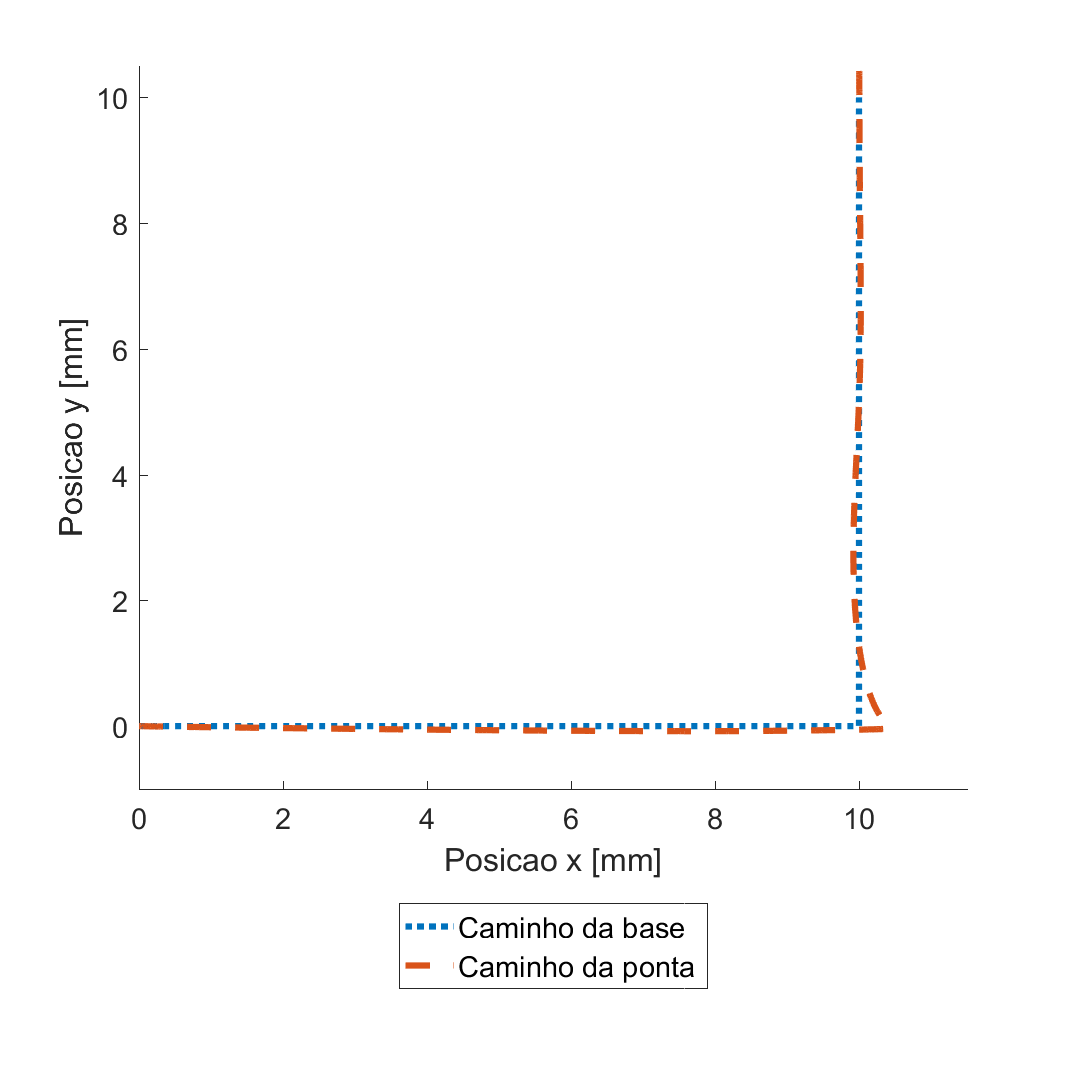
\includegraphics[width=0.47\textwidth]{Sim ref_cam_s.png}
        \label{fig:ref_cam_s}
    }
    \hfill
    \subfigure[Com controle.]{
        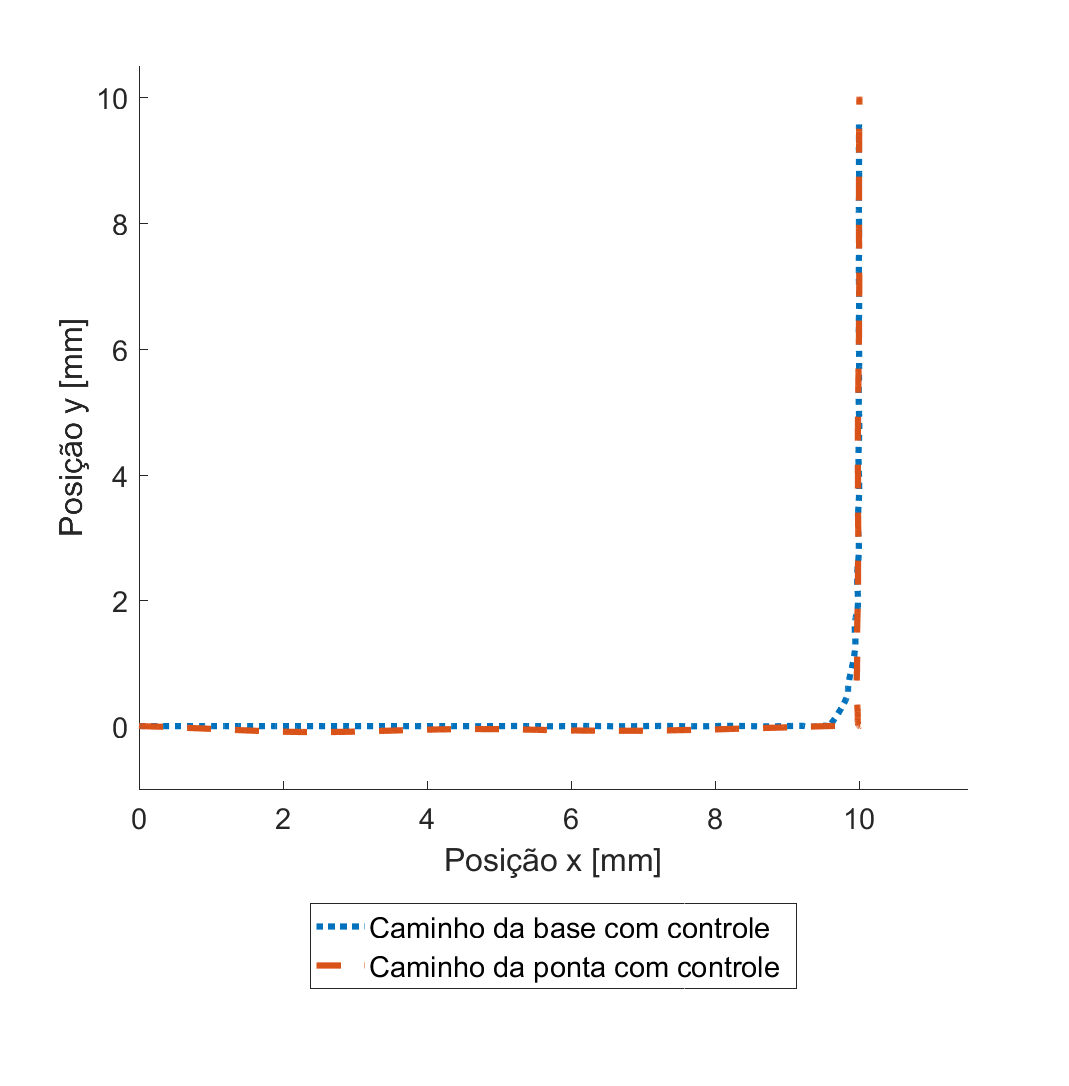
\includegraphics[width=0.47\textwidth]{Sim ref_cam_c.png}
        \label{fig:ref_cam_c}
    }
    \hfill
    \subfigure[Detalhamento - Sem controle.]{
        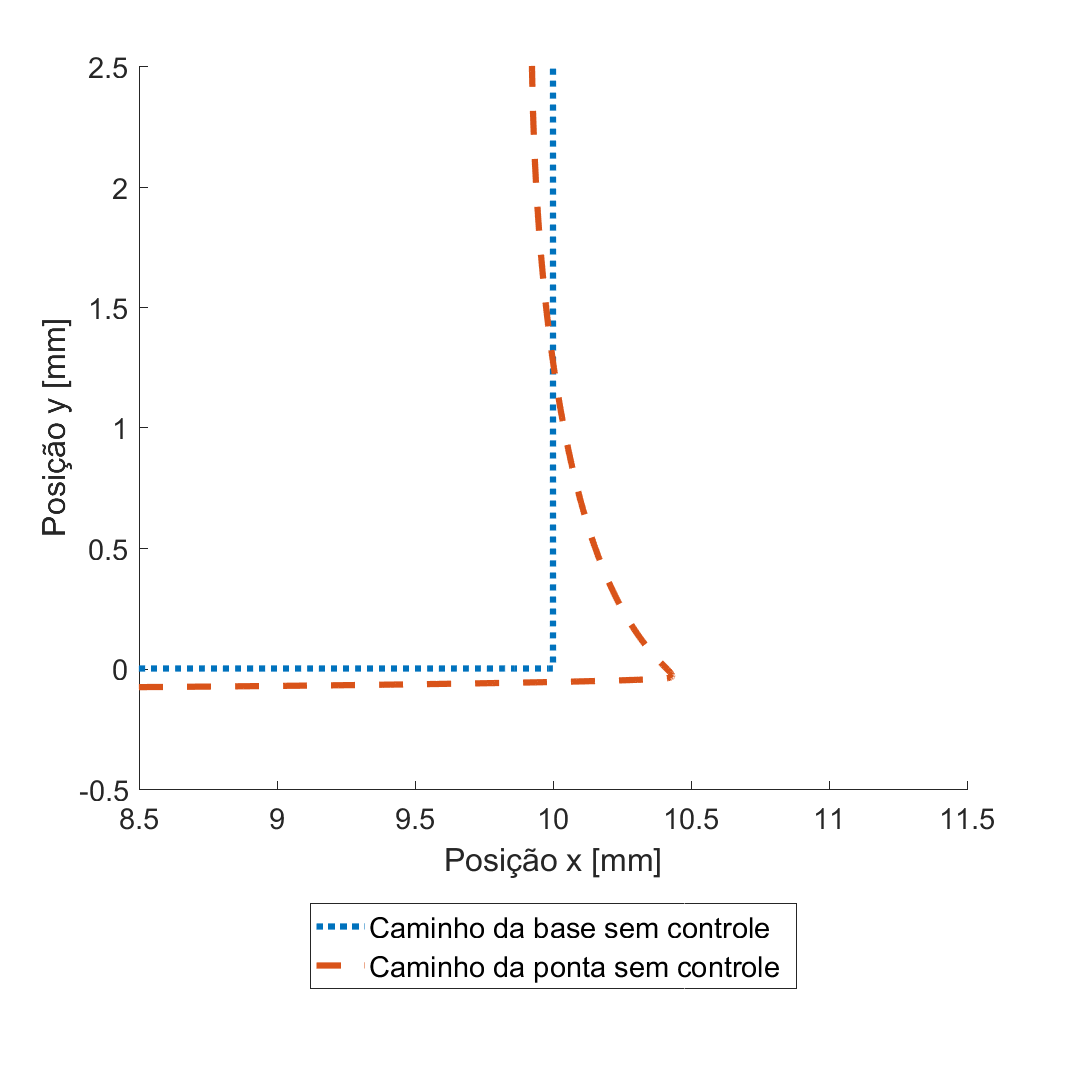
\includegraphics[width=0.47\textwidth]{Sim ref_cam_s_zoom.png}
        \label{fig:ref_cam_s_zoom}
    }
    \hfill
    \subfigure[Detalhamento - Com controle.]{
        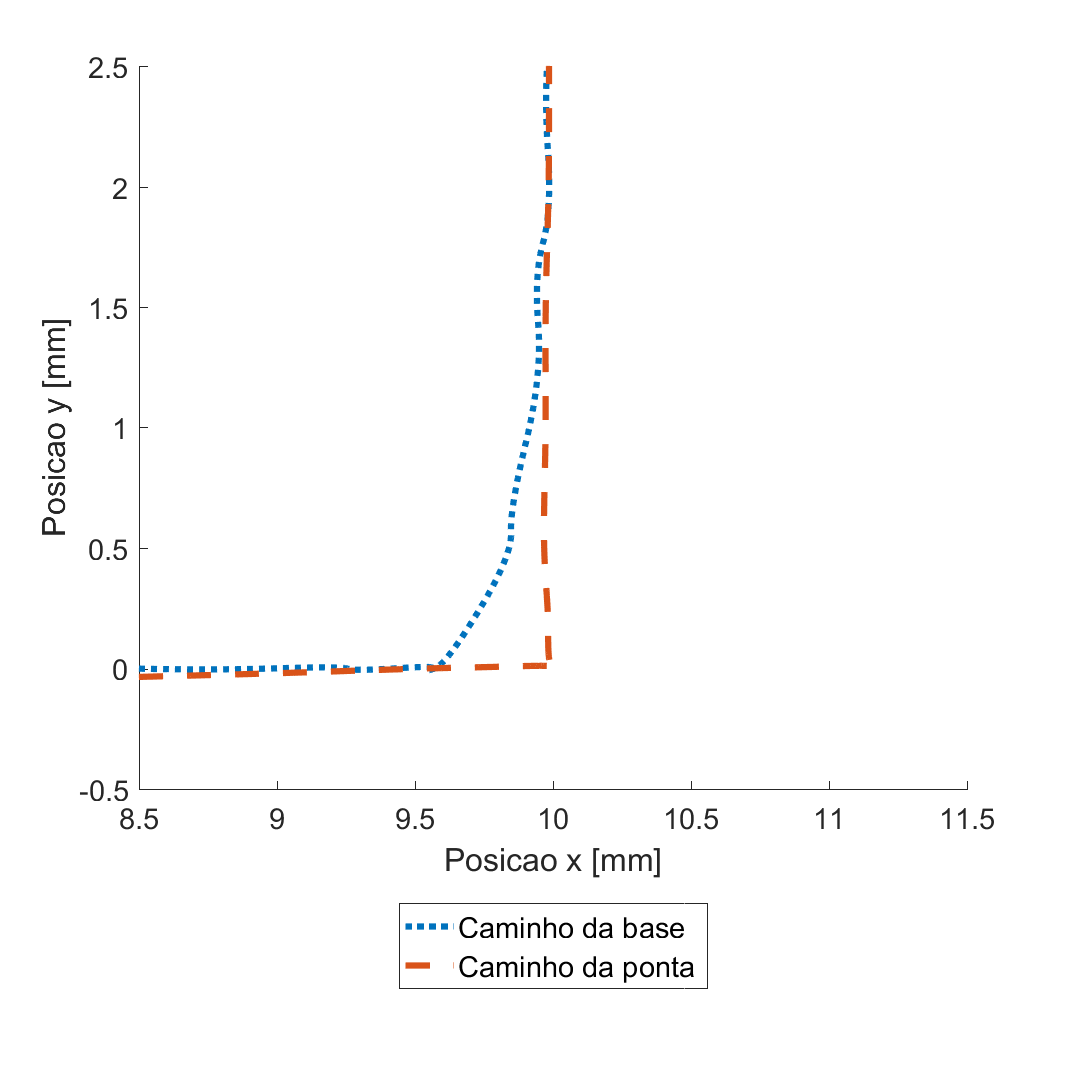
\includegraphics[width=0.47\textwidth]{Sim ref_cam_c_zoom.png}
        \label{fig:ref_cam_c_zoom}
    }
    \caption{Caminhos da ponta e da base - Referência.}
    \label{fig:ref_cam}
\end{figure}

% ------------------ Deslocamento ----------------
Na Figura \ref{fig:ref_des}, gráfico de deslocamento por tempo das curvas da base e da ponta com e sem controle dos eixos X e Y, é visível alguns comportamentos dinâmicos das curvas de deslocamento. No início do movimento, a curva da base com controle se desloca mais rapidamente, também sendo possível observar algumas oscilações. Enquanto a curva da ponta sem controle apresenta uma velocidade menor, identificada pela inclinação da curva de deslocamento, característica essa evitada pelo controle de trajetória, resultando em uma curva mais suave e com um sobre-sinal reduzido para o deslocamento da ponta com controle.

% fig:des
\begin{figure}[H]
    \centering
    \subfigure[Sem controle.]{
        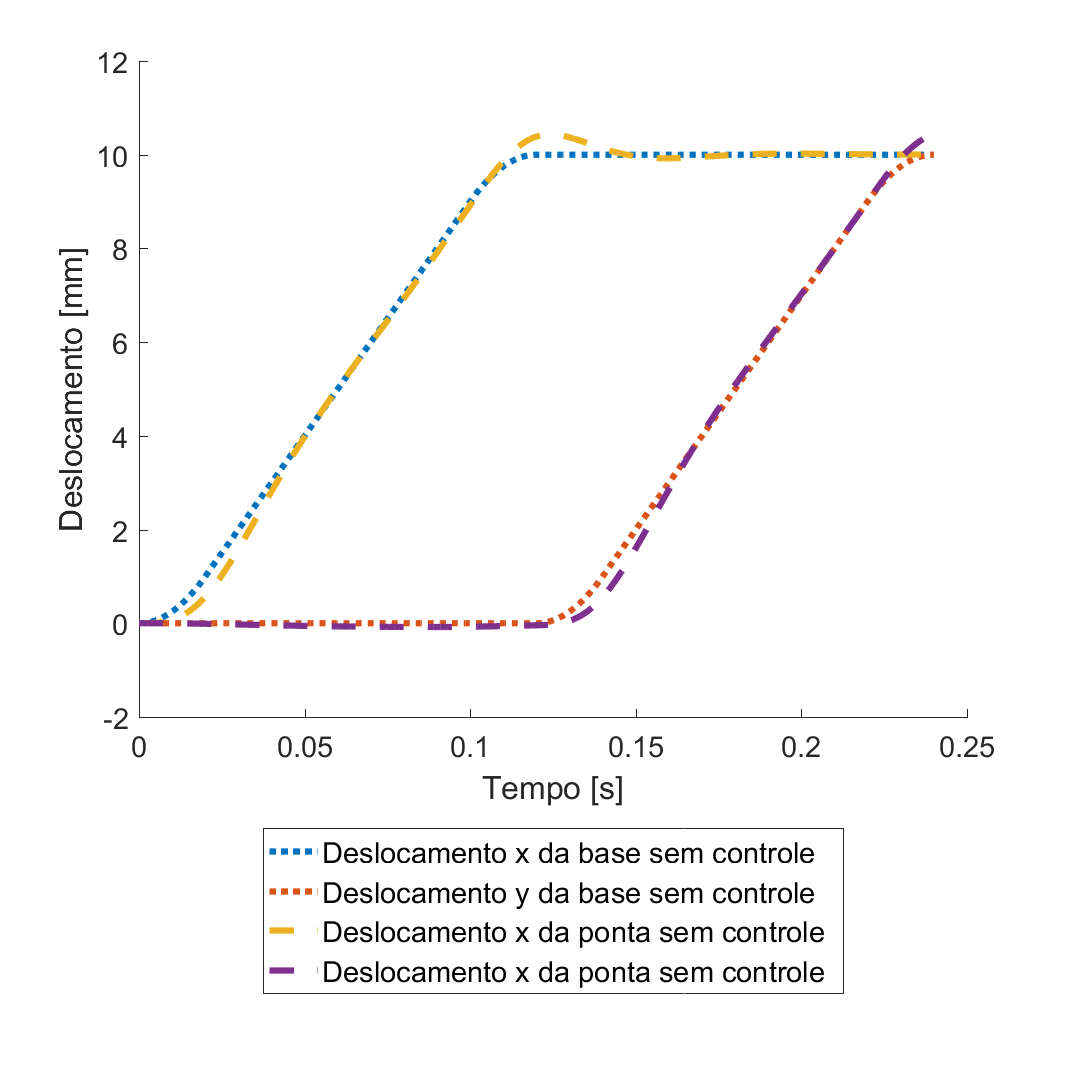
\includegraphics[width=0.47\textwidth]{Sim ref_des_s.png}
        \label{fig:ref_des_s}
    }
    \hfill
    \subfigure[Com controle.]{
        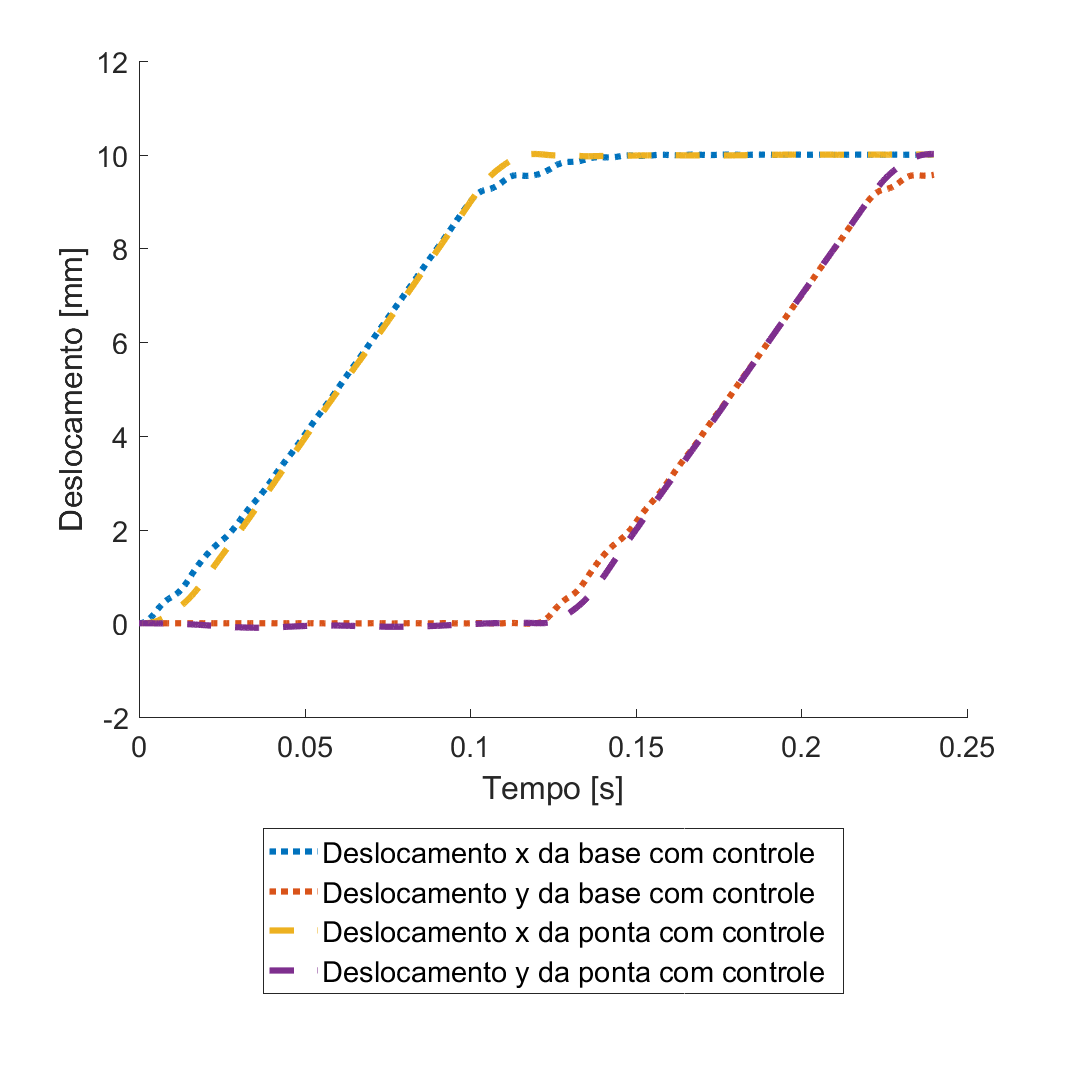
\includegraphics[width=0.47\textwidth]{Sim ref_des_c.png}
        \label{fig:ref_des_c}
    }
    \caption{Deslocamentos da ponta e da base - Referência.}
    \label{fig:ref_des}
\end{figure}

% ------------------ Velocidades ----------------
No gráfico de velocidades da base e da ponta, com e sem controle nos eixos X e Y (Figura \ref{fig:ref_vel}), observa-se um atraso da curva da ponta sem controle, quando comparado com a curva da base sem controle. Além disso, nota-se um sobre-sinal da velocidade, ambas características da elasticidade do sistema.
Já nas curvas com controle, a curva da base possui um comportamento oscilatório que vai decaindo após a perturbação, que está em fase oposta às oscilações da curva da ponta com controle. Tal comportamento tem como resultado uma diminuição do sobre sinal. Um outro fator presente no gráfico com controle é a oscilação abrupta da curva da base de velocidade, essa característica é causada por uma amostragem reduzida na etapa de geração de trajetória, fornecendo uma menor quantidade de pontos para a etapa de controle.

% fig:vel
\begin{figure}[H]
    \centering
    \subfigure[Sem controle.]{
        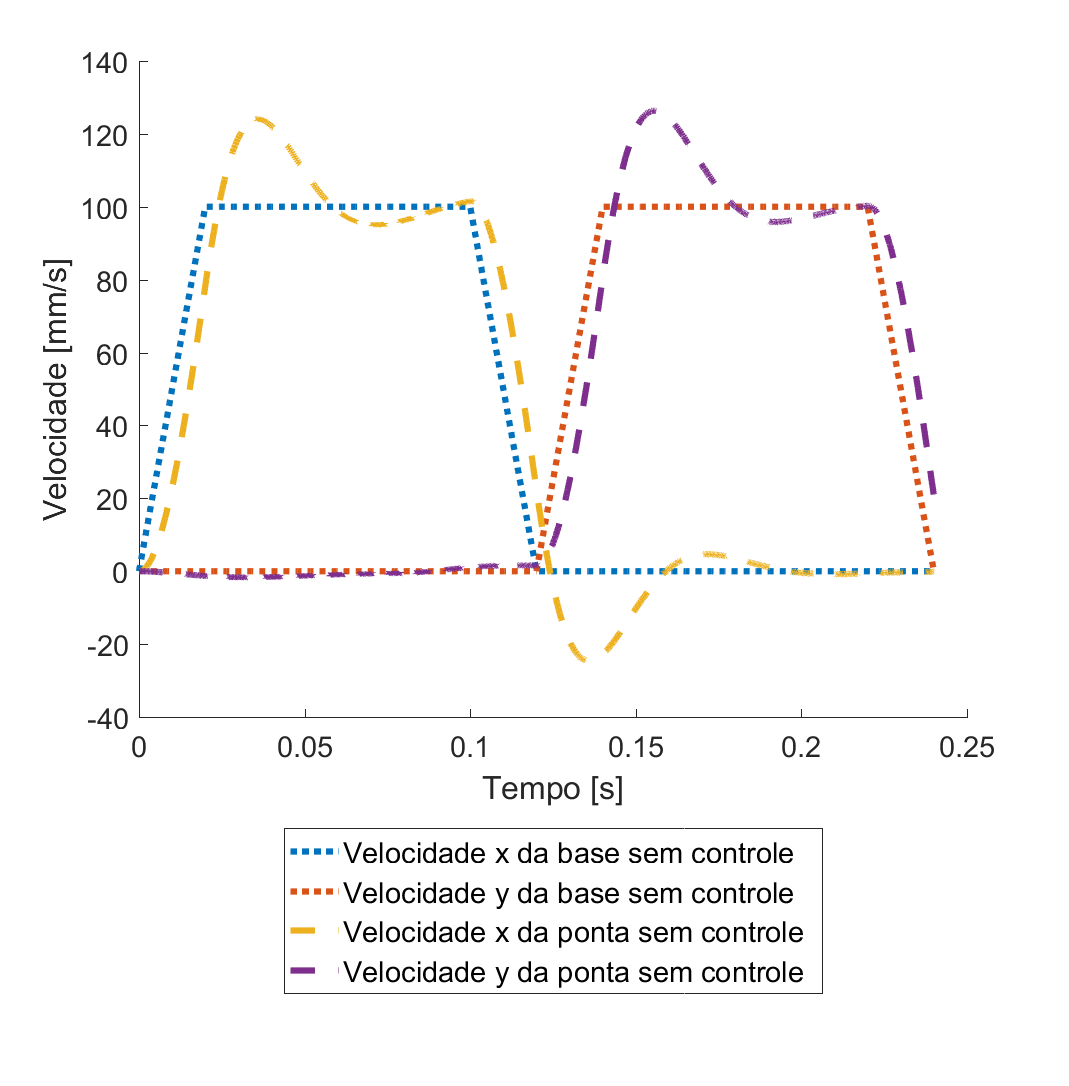
\includegraphics[width=0.47\textwidth]{Sim ref_vel_s.png}
        \label{fig:ref_vel_s}
    }
    \hfill
    \subfigure[Com controle.]{
        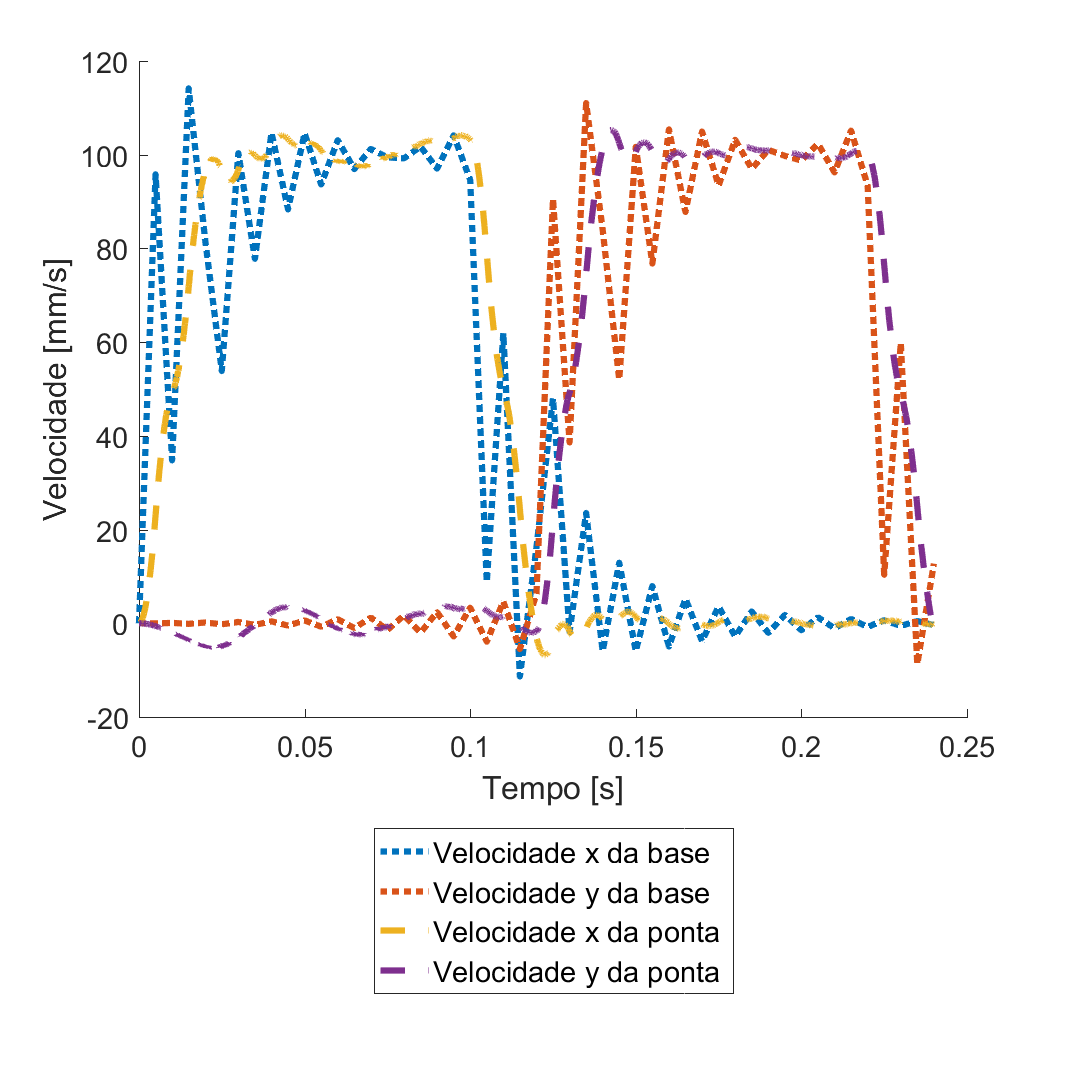
\includegraphics[width=0.47\textwidth]{Sim ref_vel_c.png}
        \label{fig:ref_vel_c}
    }
    \caption{Velocidades da ponta e da base - Referência.}
    \label{fig:ref_vel}
\end{figure}

% ------------------ end ----------------

\subsection{Caso 1 - Variação da frequência natural}
A partir desta seção são avaliados os resultados das simulações com a variação dos parâmetros, com seus valores inferiores (A) e superiores (B), comparando com os resultados da simulação referência, estes apresentados na seção anterior.

% ------------------ Caminho A ----------------

Neste primeiro gráfico (Figura \ref{fig:1A_cam}) é apresentado os caminhos da base e da ponta, com e sem controle no plano XY com o parâmetro da frequência natural em seu nível inferior, definido como \(50 rad/s\). Nota-se algumas características em comum com a Figura \ref{fig:ref_cam} dos caminhos da simulação referência, mas o caminho da ponta sem controle apresenta um desvio maior se comparado ao caminho da ponta sem controle de referência, efeito esse causado pela menor rigidez do sistema. Por consequência, nota-se que foi necessário uma compensação mais agressiva do caminho da base com controle, derivado dessa menor rigidez e maior desvio. Sendo que, em um momento o movimento no eixo X da base com controle precisou mudar de direção. Apesar deste maior desvio na curva sem controle, o caminho da ponta com controle apresenta um desvio similar à simulação de referência.

% fig:cam
\begin{figure}[H]
    \centering
    \subfigure[Sem controle.]{
        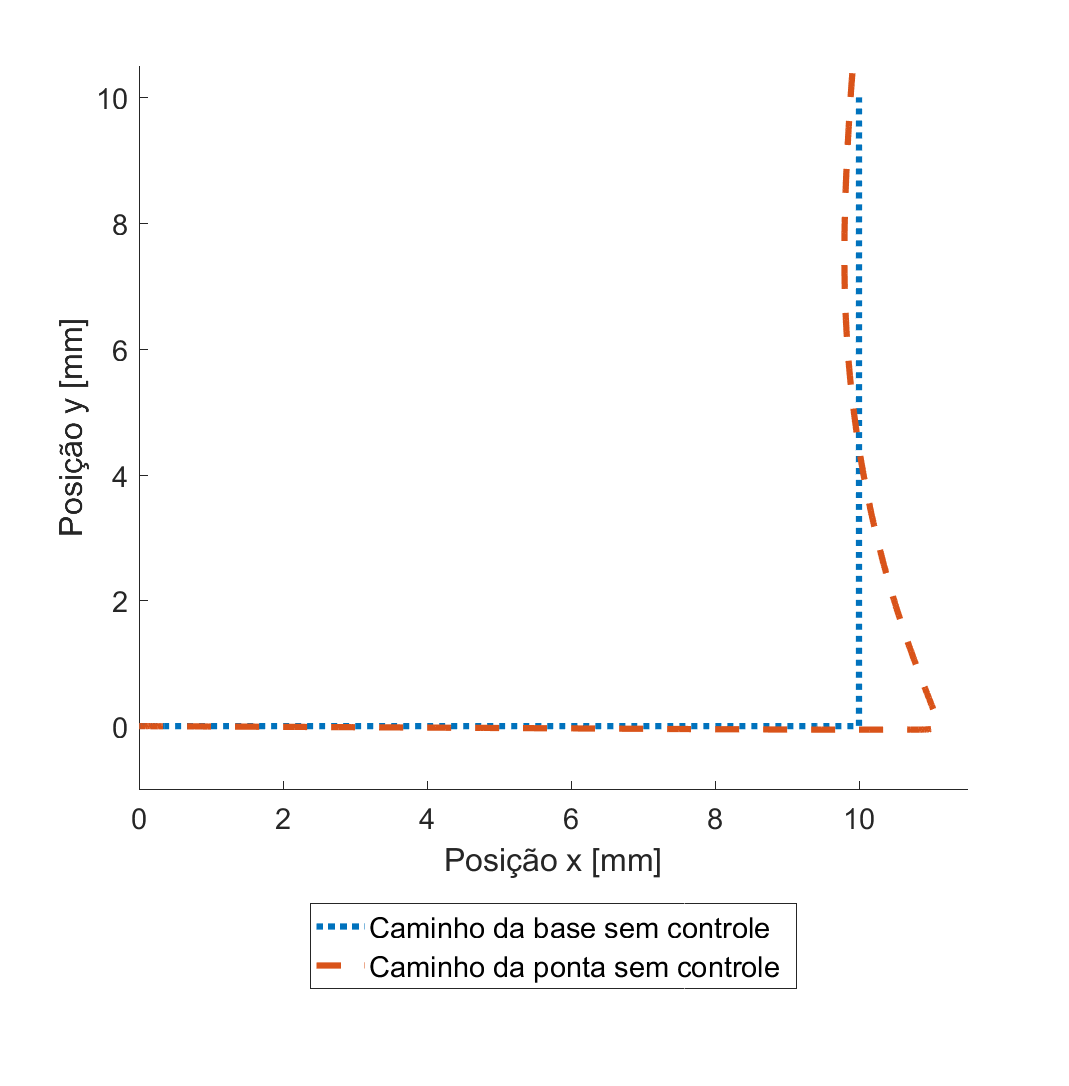
\includegraphics[width=0.47\textwidth]{Sim 1A_cam_s.png}
        \label{fig:1A_cam_s}
    }
    \hfill
    \subfigure[Com controle.]{
        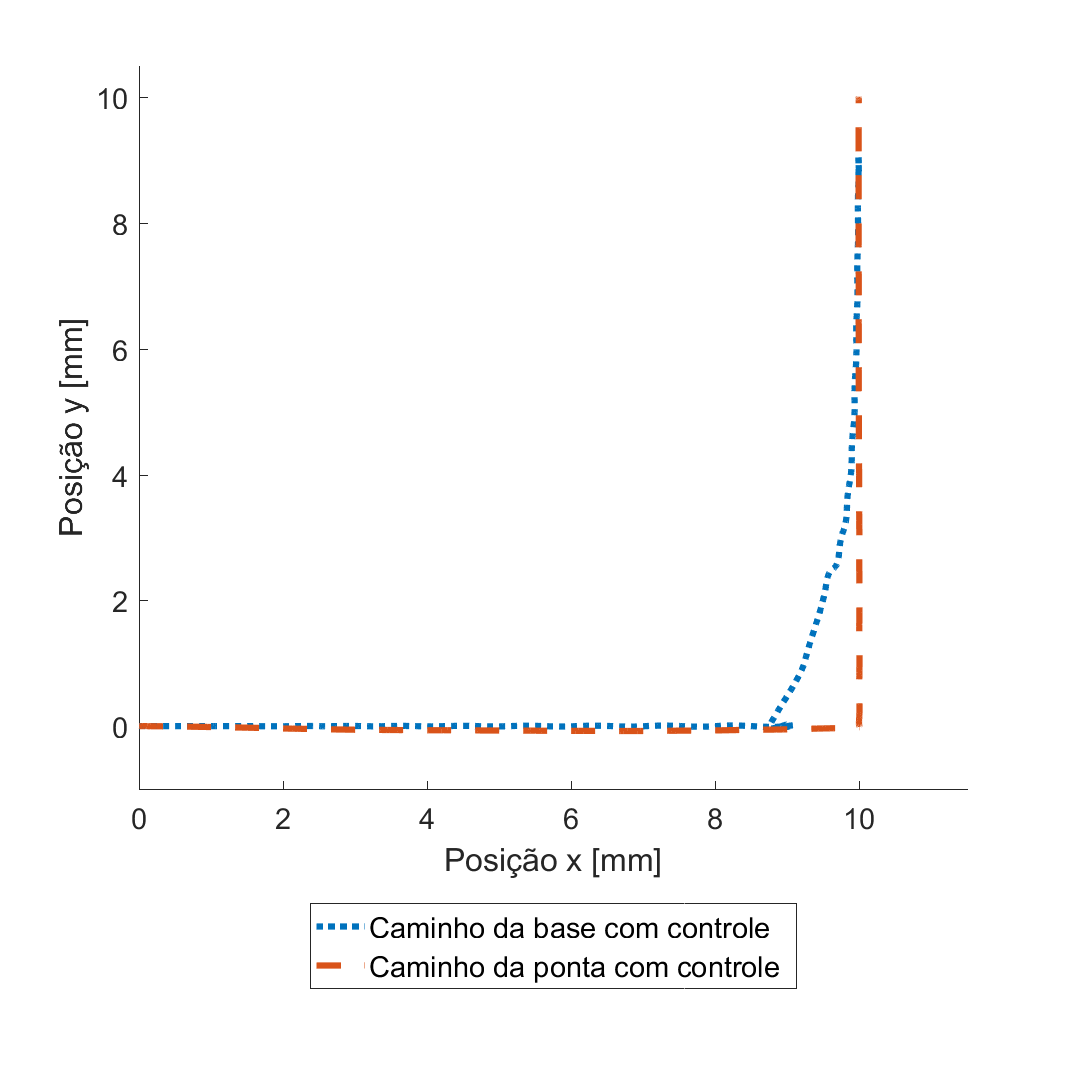
\includegraphics[width=0.47\textwidth]{Sim 1A_cam_c.png}
        \label{fig:1A_cam_c}
    }
    \hfill
    \subfigure[Detalhamento - Sem controle.]{
        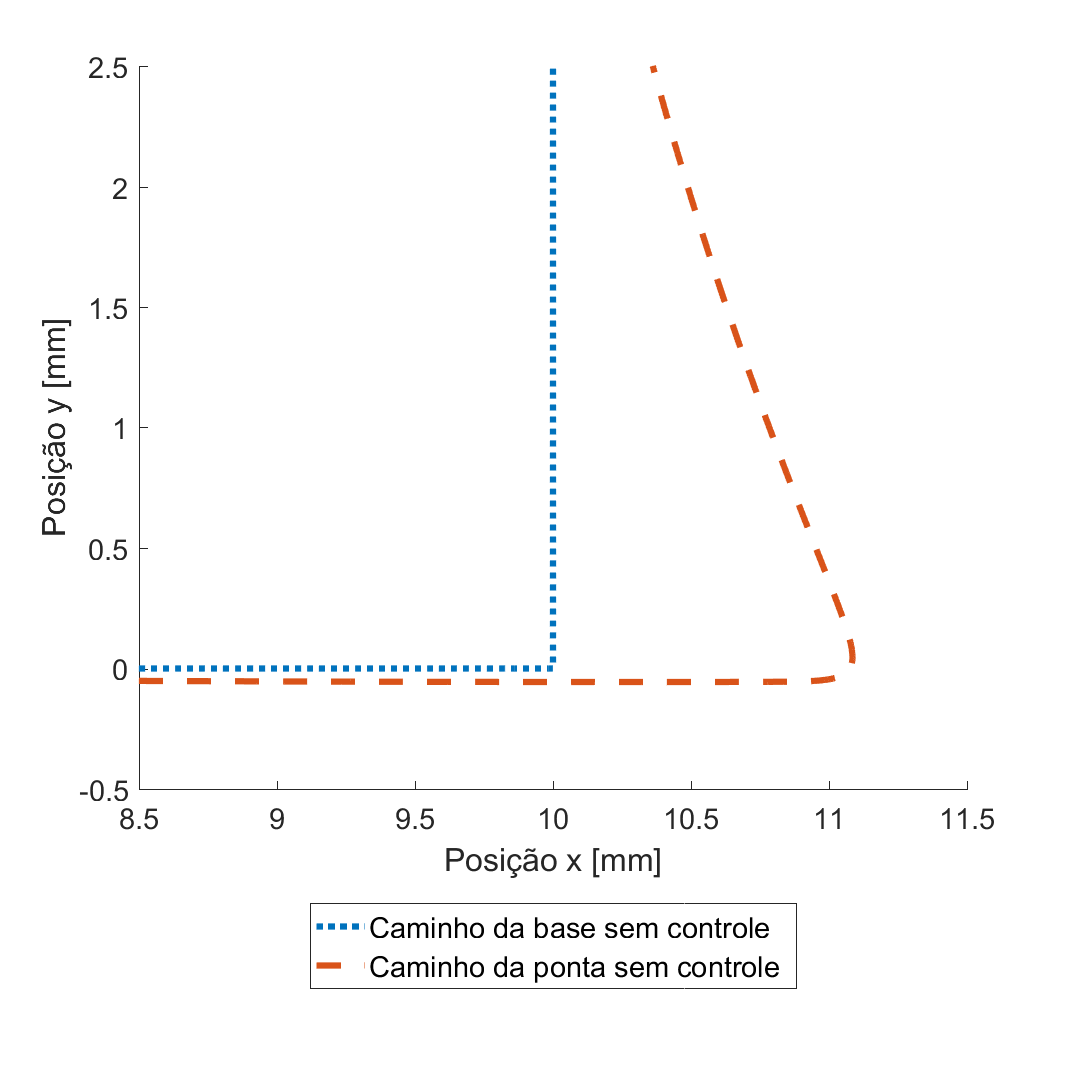
\includegraphics[width=0.47\textwidth]{Sim 1A_cam_s_zoom.png}
        \label{fig:1A_cam_s_zoom}
    }
    \hfill
    \subfigure[Detalhamento - Com controle.]{
        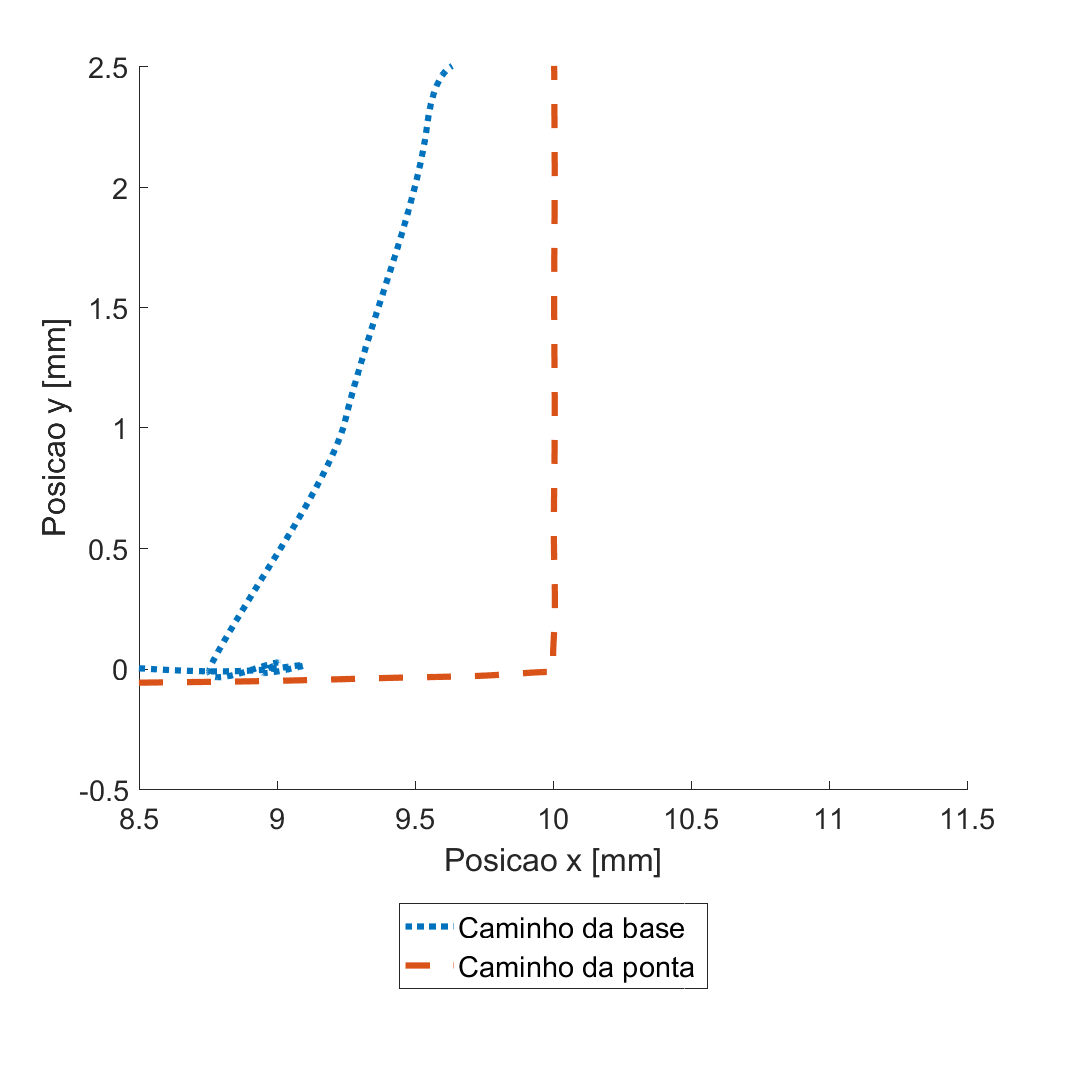
\includegraphics[width=0.47\textwidth]{Sim 1A_cam_c_zoom.png}
        \label{fig:1A_cam_c_zoom}
    }
    \caption{Caminhos da ponta e da base - Caso 1A.}
    \label{fig:1A_cam}
\end{figure}

% ------------------ Deslocamento A----------------
Neste gráfico (Figura \ref{fig:1A_des}) estão representados os deslocamentos em X e Y da base e da ponta, tanto da simulação sem controle e com controle. Aqui nota-se de maneira mais clara, a mudança de direção no eixo X próximo a 9 mm, causado pela necessidade de se compensar a elasticidade do sistema desta simulação.

% fig:des
\begin{figure}[H]
    \centering
    \subfigure[Sem controle.]{
        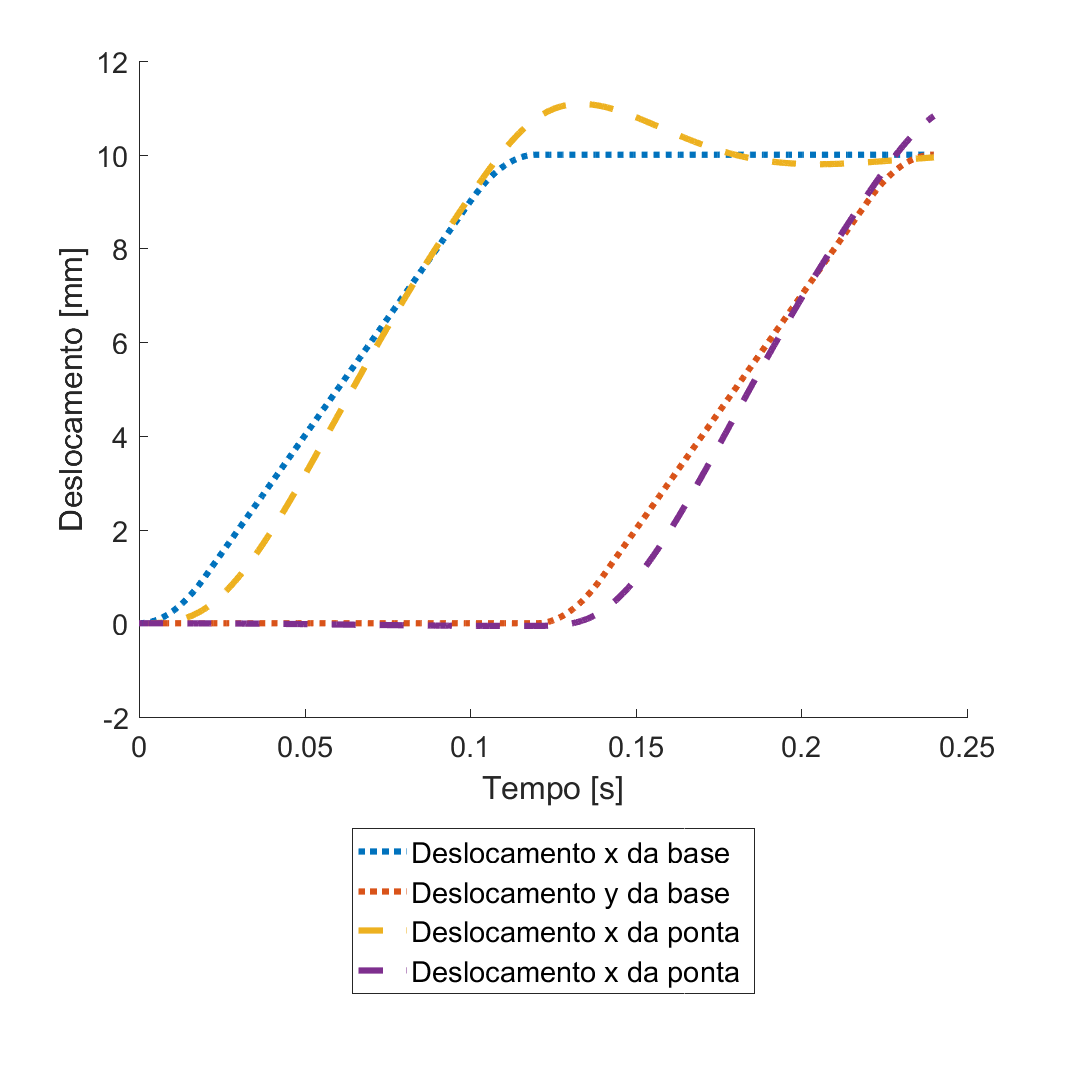
\includegraphics[width=0.47\textwidth]{Sim 1A_des_s.png}
        \label{fig:1A_des_s}
    }
    \hfill
    \subfigure[Com controle.]{
        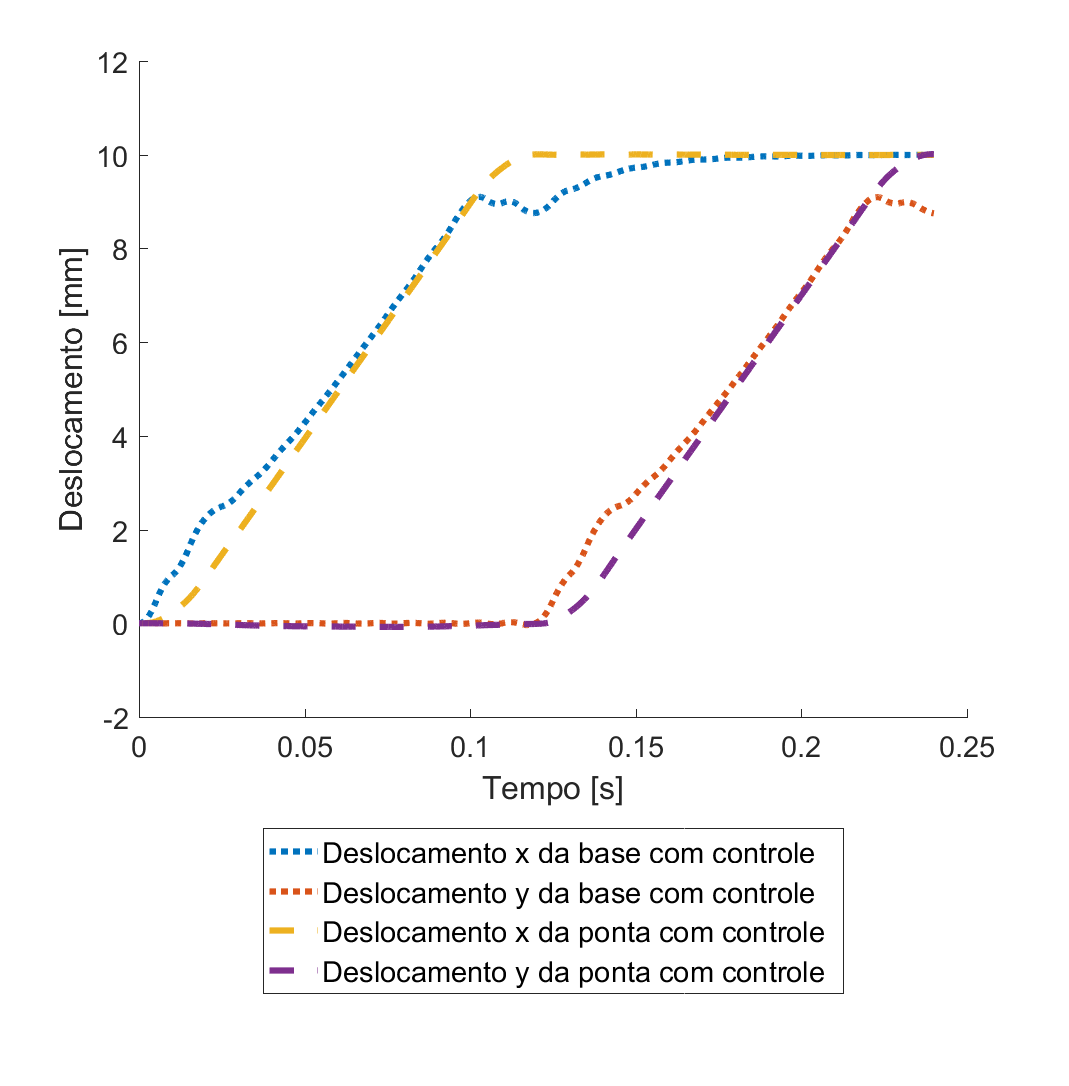
\includegraphics[width=0.47\textwidth]{Sim 1A_des_c.png}
        \label{fig:1A_des_c}
    }
    \caption{Deslocamentos da ponta e da base - Caso 1A.}
    \label{fig:1A_des}
\end{figure}

% ------------------ Velocidades A ----------------
Já nos gráficos de velocidade, apresentados na Figura \ref{fig:1A_vel}, observa-se um atraso maior do perfil de velocidade da ponta sem controle em relação ao perfil da base sem controle, quando comparado à simulação de referência. E portanto, o caráter do perfil de velocidades da base com controle é mais agressivo, ou seja, possui oscilações com uma maior amplitude, de forma a amenizar a amplitude das oscilações do perfil de velocidade da ponta com controle.
% fig:vel
\begin{figure}[H]
    \centering
    \subfigure[Sem controle.]{
        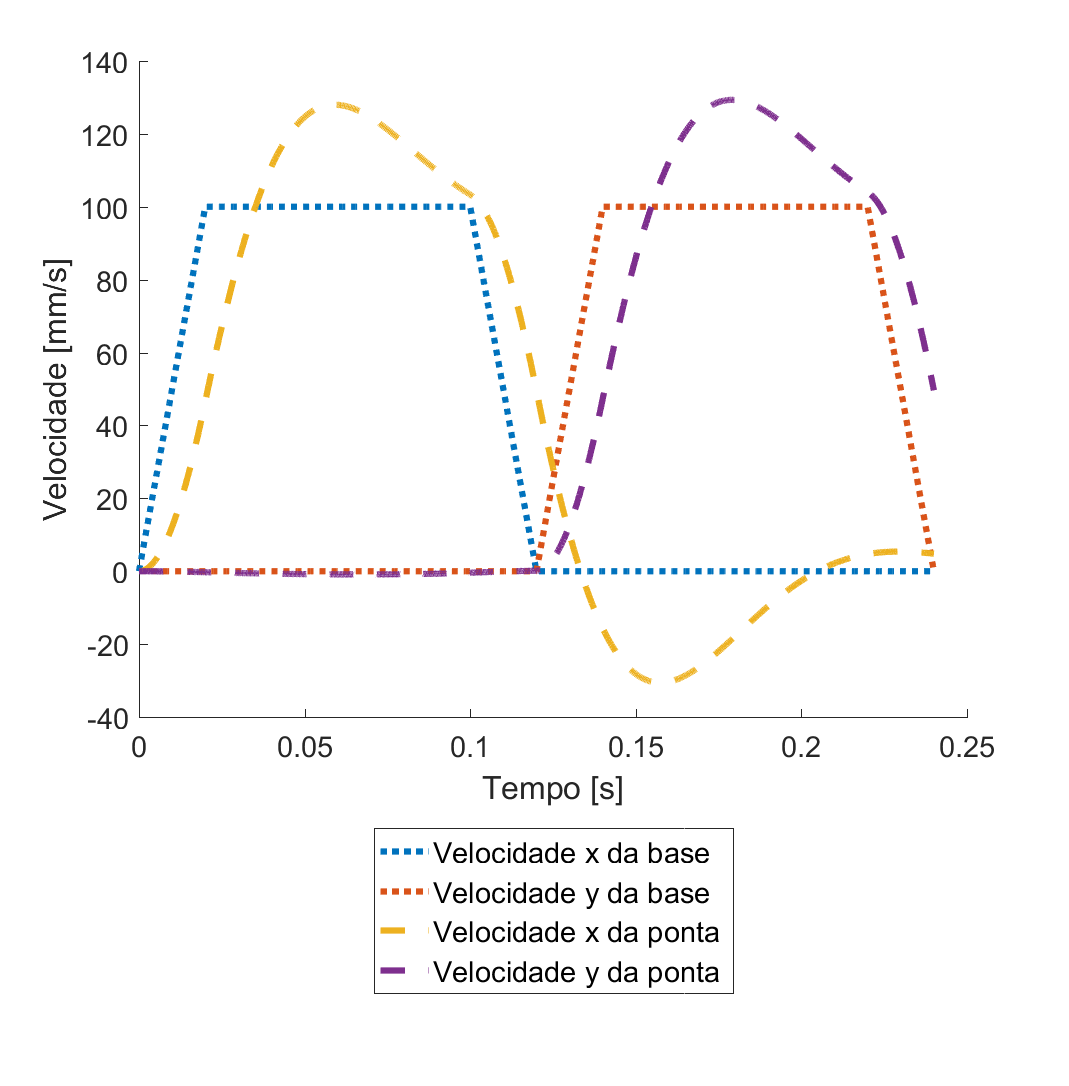
\includegraphics[width=0.47\textwidth]{Sim 1A_vel_s.png}
        \label{fig:1A_vel_s}
    }
    \hfill
    \subfigure[Com controle.]{
        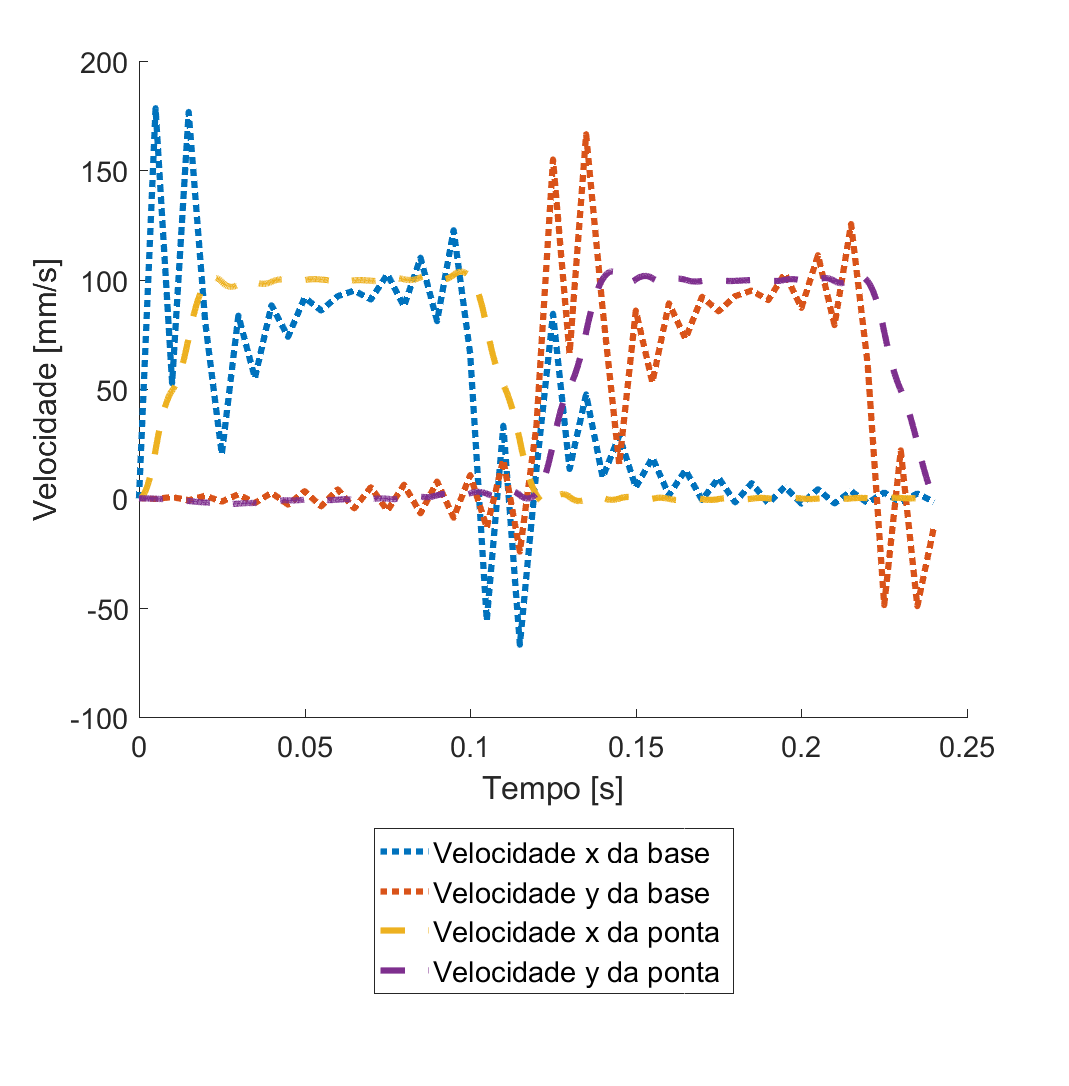
\includegraphics[width=0.47\textwidth]{Sim 1A_vel_c.png}
        \label{fig:1A_vel_c}
    }
    \caption{Velocidades da ponta e da base - Caso 1A.}
    \label{fig:1A_vel}
\end{figure}
% ------------------ Caminho B ----------------

Agora, avaliando a simulação da variação do parâmetro de frequência natural com o valor B (\(200 rad/s\)) é notável a redução do desvio no caminho da ponta sem controle (Figura \ref{fig:1B_cam}), característica coerente com o aumento da rigidez do sistema. Entretanto, o desvio do caminho da ponta com controle aumentou se comparado à simulação de referência. Este efeito pode ser causado por conta da interação entre o passo de tempo de interpolação, ou seja a amostragem dos pontos, e o aumento da frequência natural, que exige uma maior densidade de pontos para representar seu comportamento. 

% fig:cam
\begin{figure}[H]
    \centering
    \subfigure[Sem controle.]{
        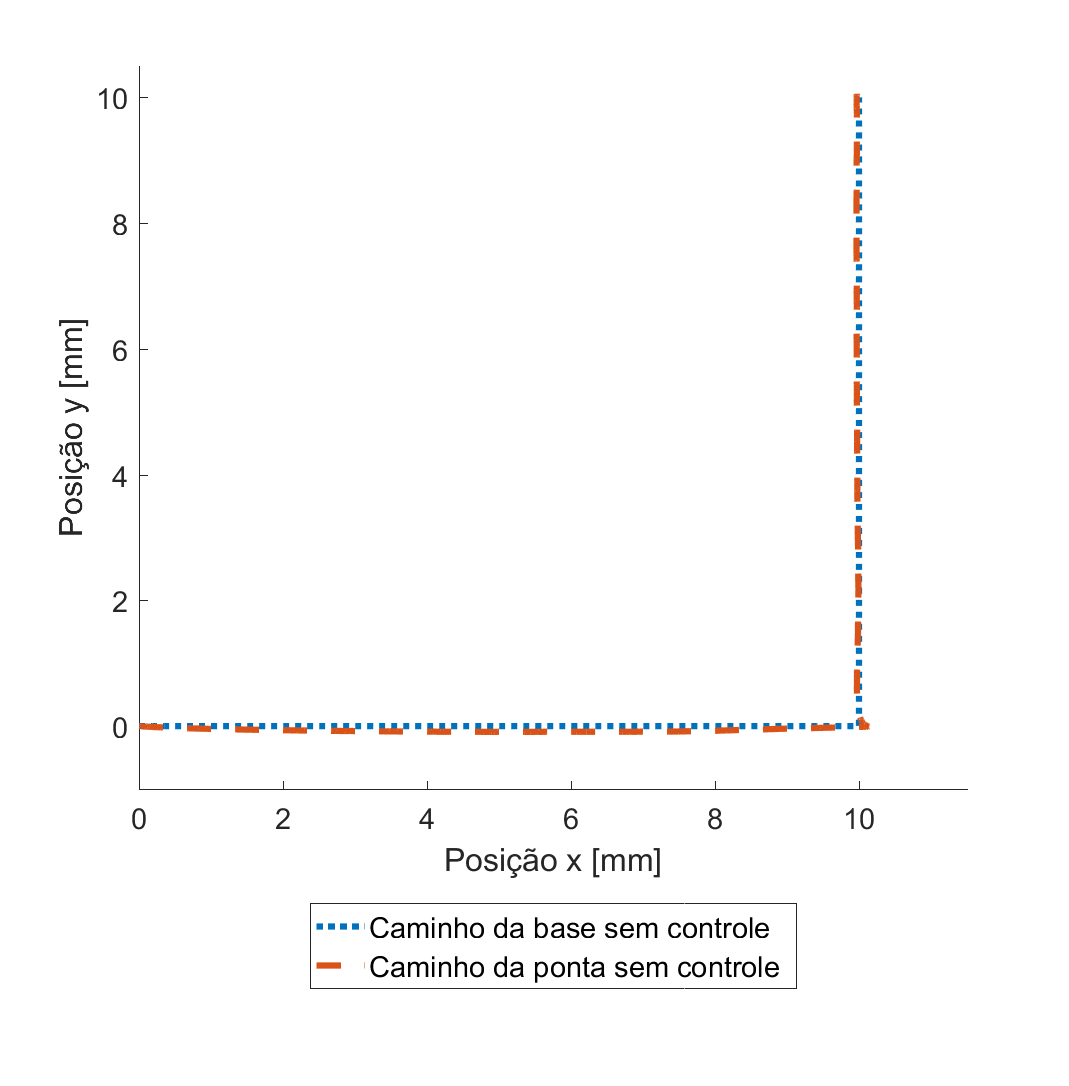
\includegraphics[width=0.47\textwidth]{Sim 1B_cam_s.png}
        \label{fig:1B_cam_s}
    }
    \hfill
    \subfigure[Com controle.]{
        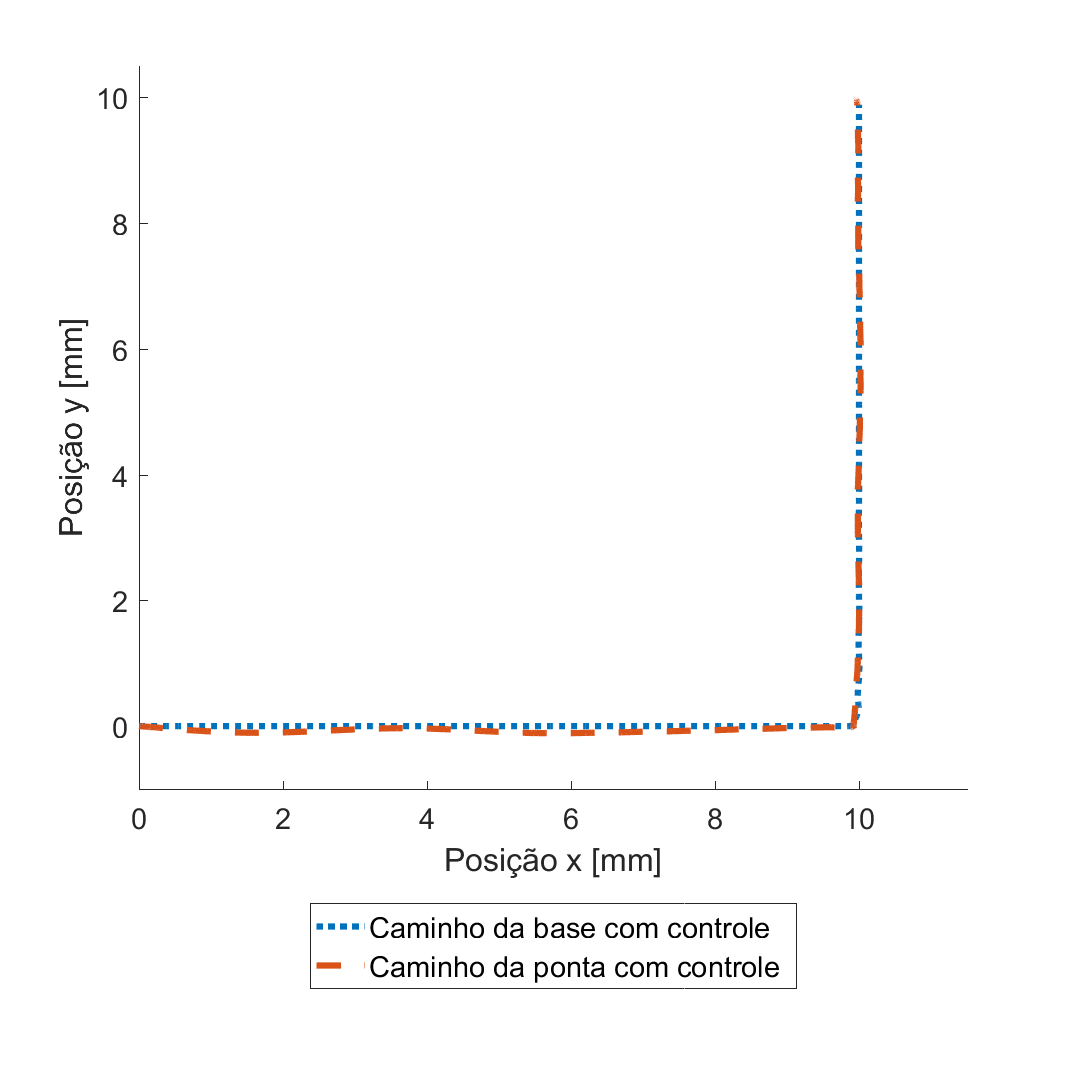
\includegraphics[width=0.47\textwidth]{Sim 1B_cam_c.png}
        \label{fig:1B_cam_c}
    }
    \hfill
    \subfigure[Detalhamento - Sem controle.]{
        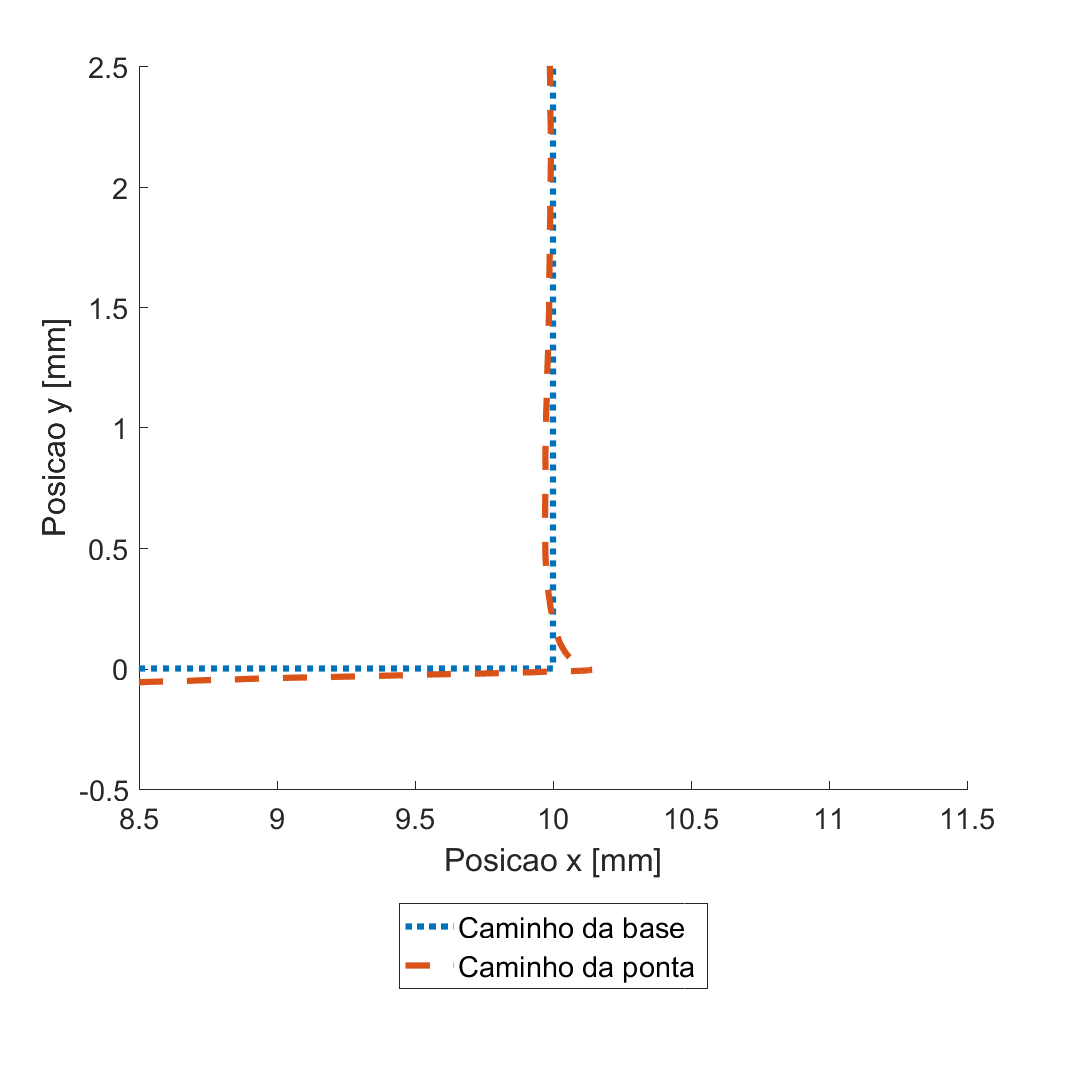
\includegraphics[width=0.47\textwidth]{Sim 1B_cam_s_zoom.png}
        \label{fig:1B_cam_s_zoom}
    }
    \hfill
    \subfigure[Detalhamento - Com controle.]{
        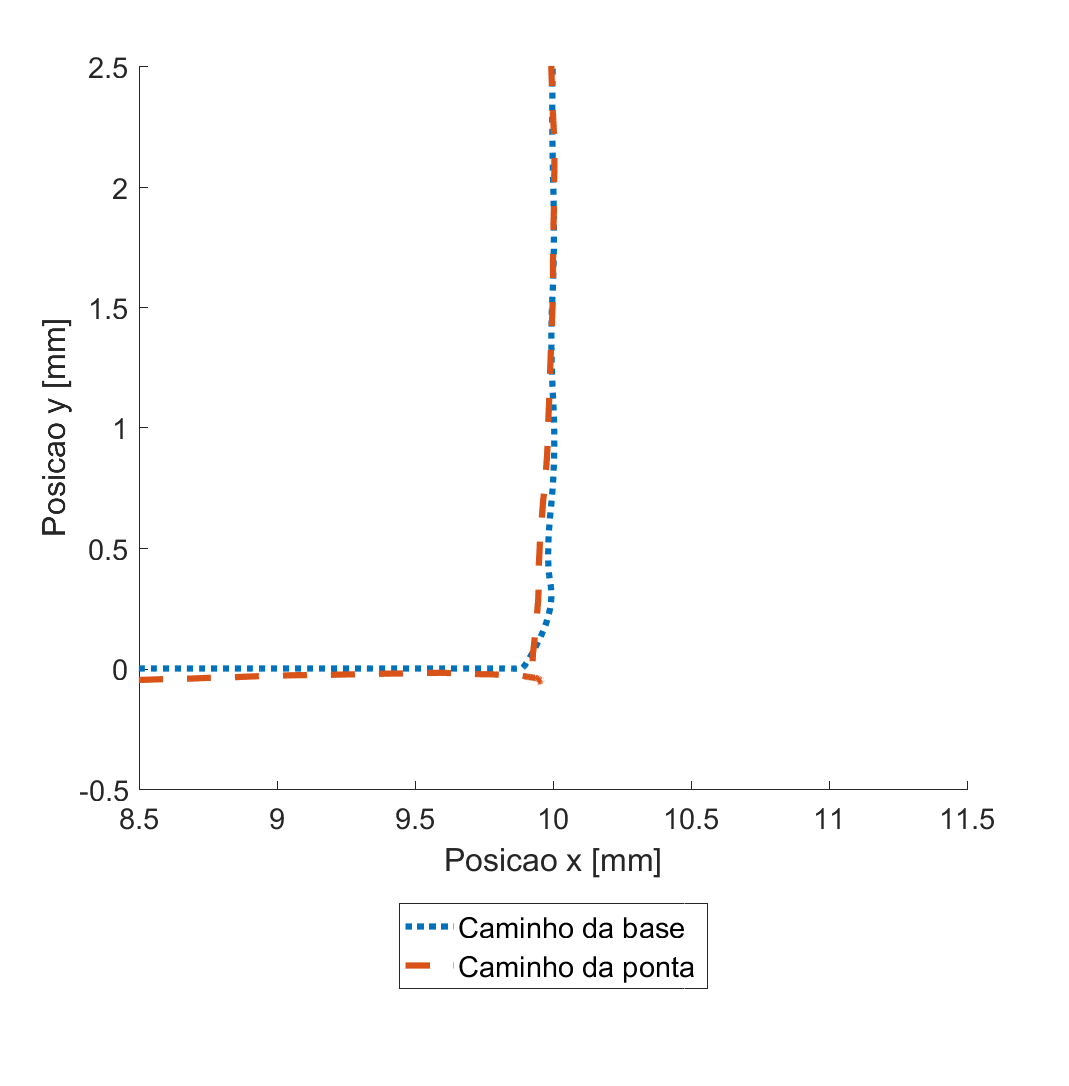
\includegraphics[width=0.47\textwidth]{Sim 1B_cam_c_zoom.png}
        \label{fig:1B_cam_c_zoom}
    }
    \caption{Caminhos da ponta e da base - Caso 1B.}
    \label{fig:1B_cam}
\end{figure}

% ------------------ Deslocamento B----------------
No gráfico de deslocamentos (Figura \ref{fig:1B_des}) as curvas da ponta e da base estão muito próximas, tanto para as curvas com controle e sem controle. Este efeito se dá pelo aumento da rigidez quando comparado às simulações anteriores.

% fig:des
\begin{figure}[H]
    \centering
    \subfigure[Sem controle.]{
        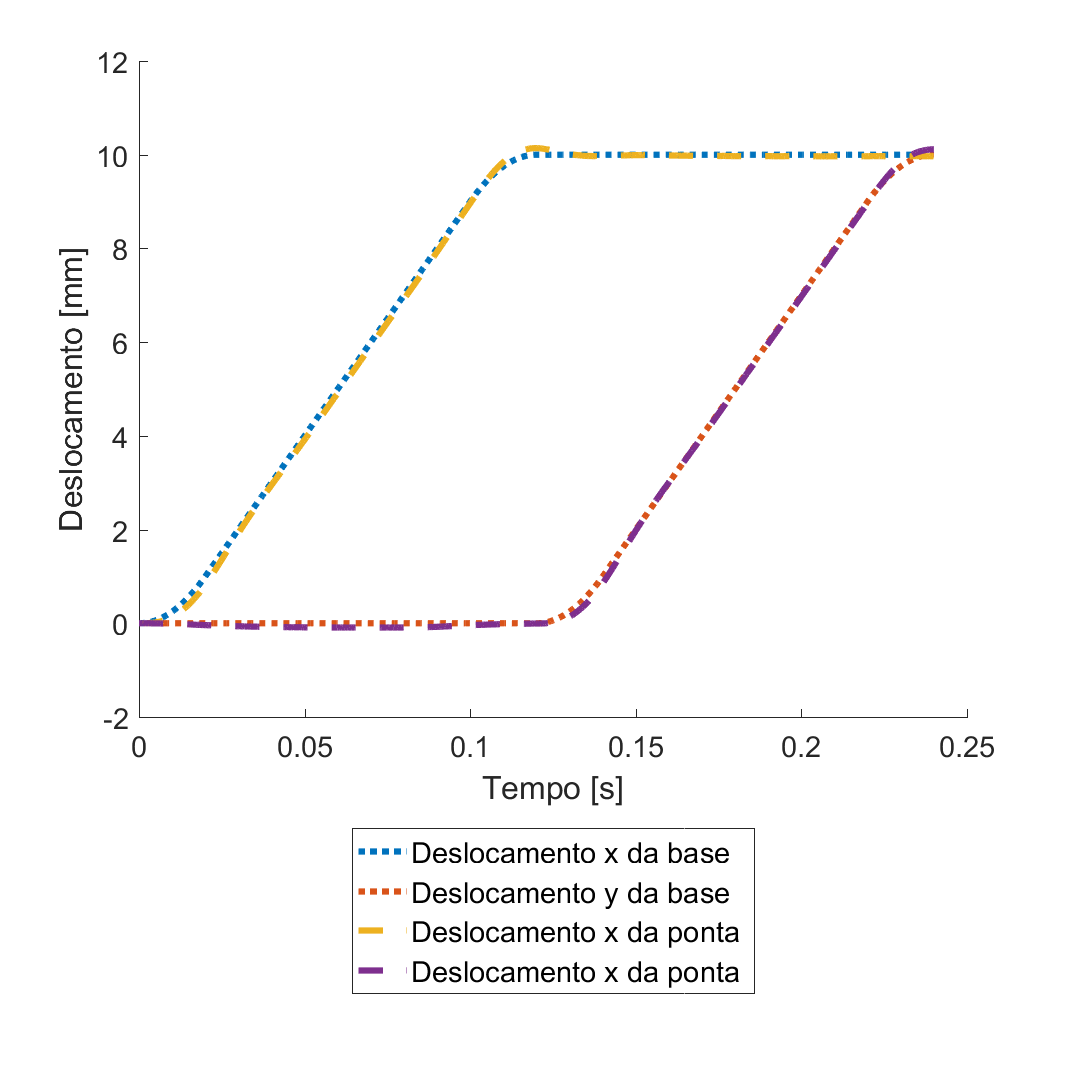
\includegraphics[width=0.47\textwidth]{Sim 1B_des_s.png}
        \label{fig:1B_des_s}
    }
    \hfill
    \subfigure[Com controle.]{
        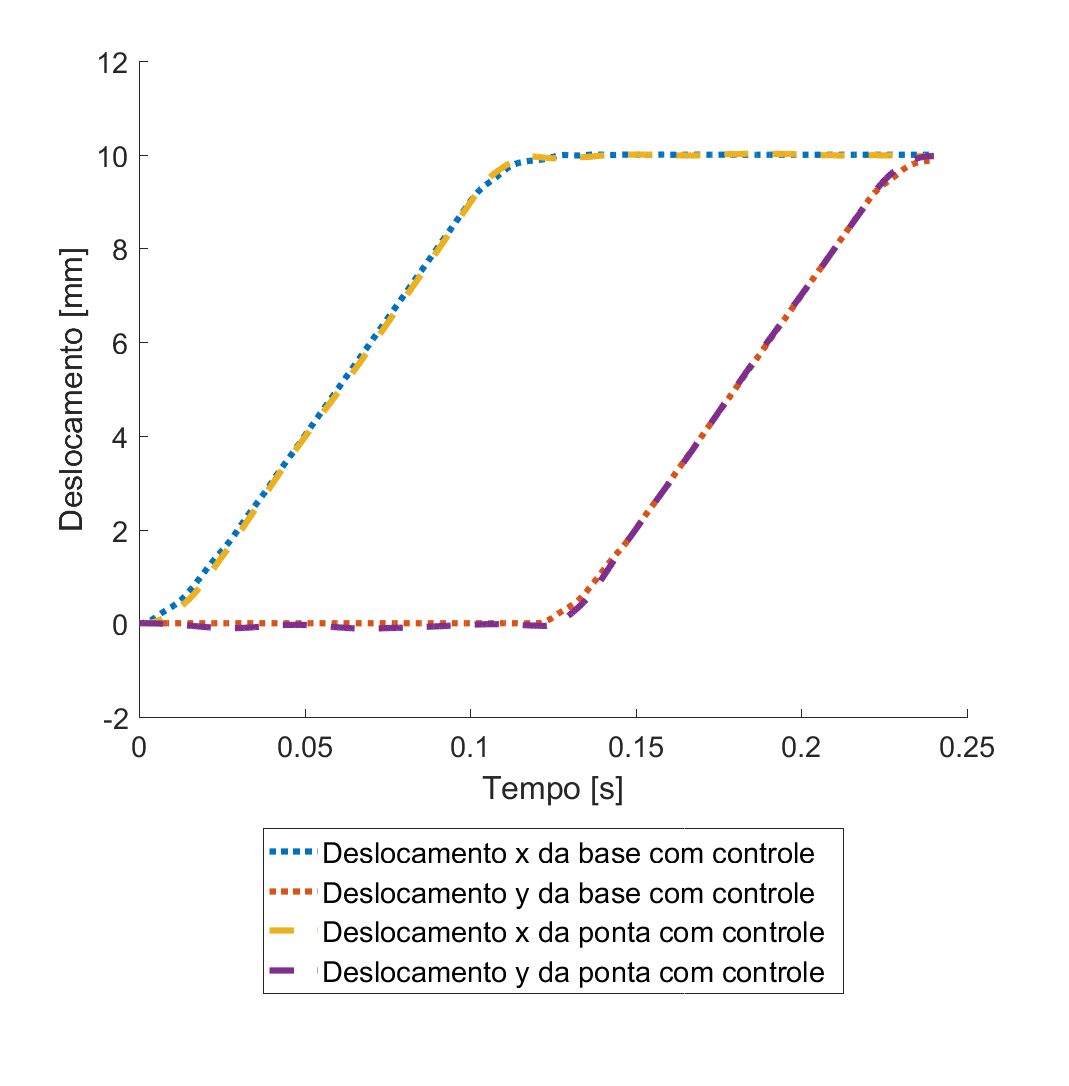
\includegraphics[width=0.47\textwidth]{Sim 1B_des_c.png}
        \label{fig:1B_des_c}
    }
    \caption{Deslocamentos da ponta e da base - Caso 1B.}
    \label{fig:1B_des}
\end{figure}

% ------------------ Velocidades B ----------------
Já na Figura \ref{fig:1B_vel}, nota-se vibrações de frequência mais alta e um sobre-sinal bem definido na curva da ponta sem controle. Enquanto que na curva da base com controle, a aceleração inicial é marcada por várias quebras e um sobre-sinal menos bem definido na curva da ponta com controle, apesar das vibrações de alta frequência se manterem.

% fig:vel
\begin{figure}[H]
    \centering
    \subfigure[Sem controle.]{
        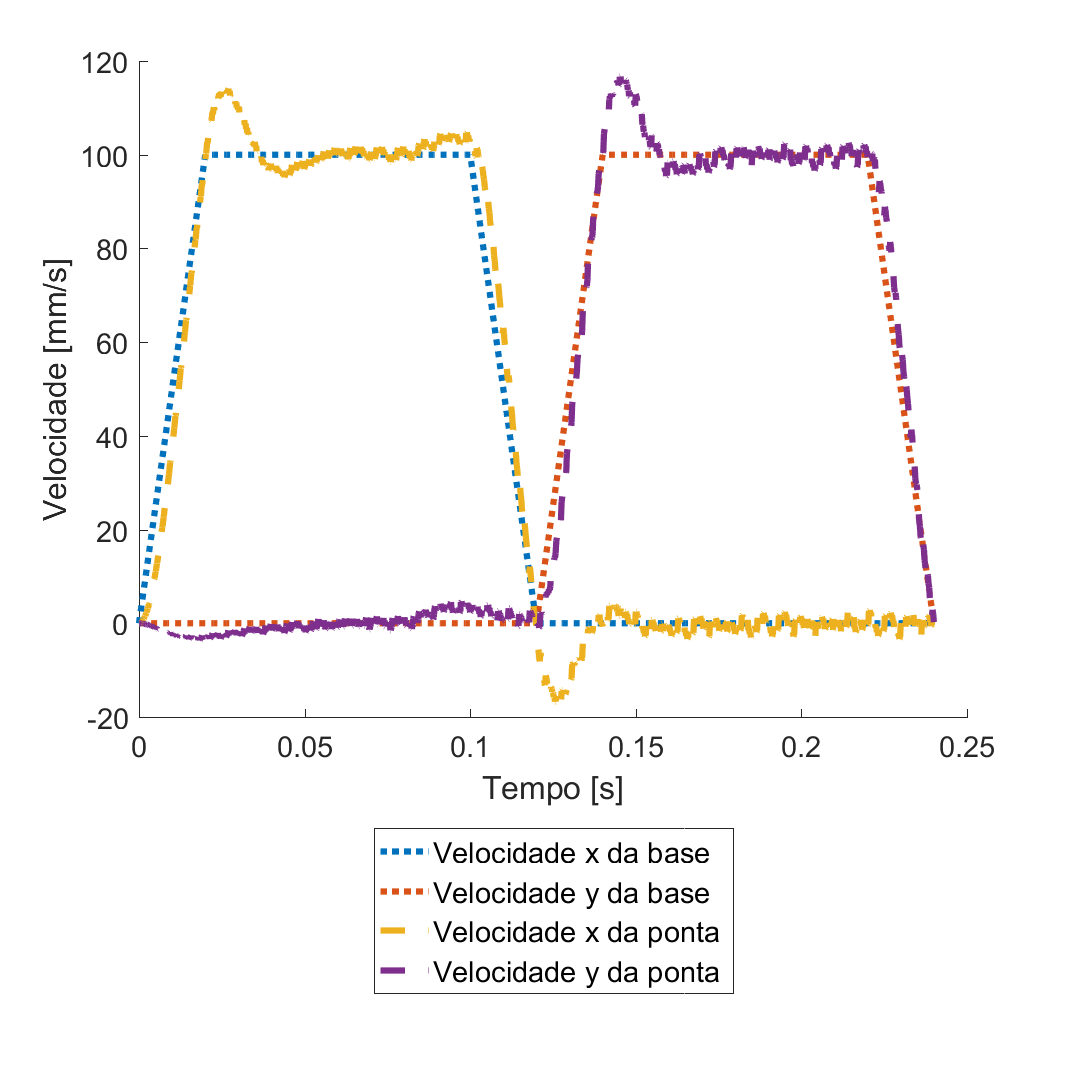
\includegraphics[width=0.47\textwidth]{Sim 1B_vel_s.png}
        \label{fig:1B_vel_s}
    }
    \hfill
    \subfigure[Com controle.]{
        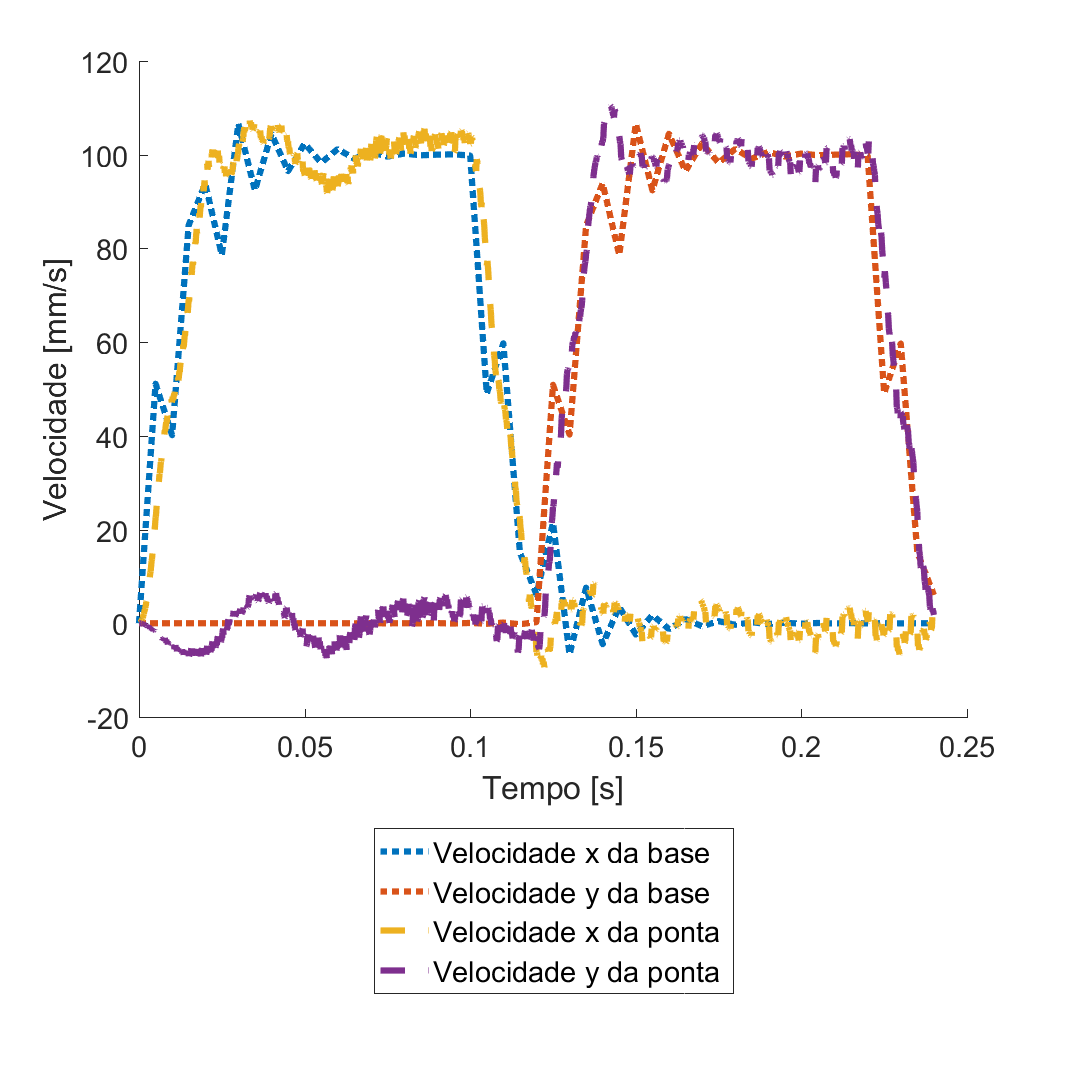
\includegraphics[width=0.47\textwidth]{Sim 1B_vel_c.png}
        \label{fig:1B_vel_c}
    }
    \caption{Velocidades da ponta e da base - Caso 1B.}
    \label{fig:1B_vel}
\end{figure}

% ------------------ end ----------------

\subsection{Caso 2 - Variação do coeficiente de amortecimento}

% ------------------ Caminho A ----------------
Diferentemente dos gráficos dos caminhos sem controle das simulações anteriores, a curva da ponta sem controle do Caso 1A (coeficiente de amortecimento \(0\)) apresenta uma oscilação que não decai ao longo do caminho após a perturbação. Isto se deve ao fato de não existir dissipação de energia no sistema fechado. Apesar deste fato, a curva da ponta com controle conseguiu se manter com um desvio pequeno, apesar de ser uma performance inferior à da simulação de referência. Estes efeitos podem ser visualizados na Figura \ref{fig:2A_cam} que apresenta os caminhos da base e da ponta para as condições com e sem controle.

% fig:cam
\begin{figure}[H]
    \centering
    \subfigure[Sem controle.]{
        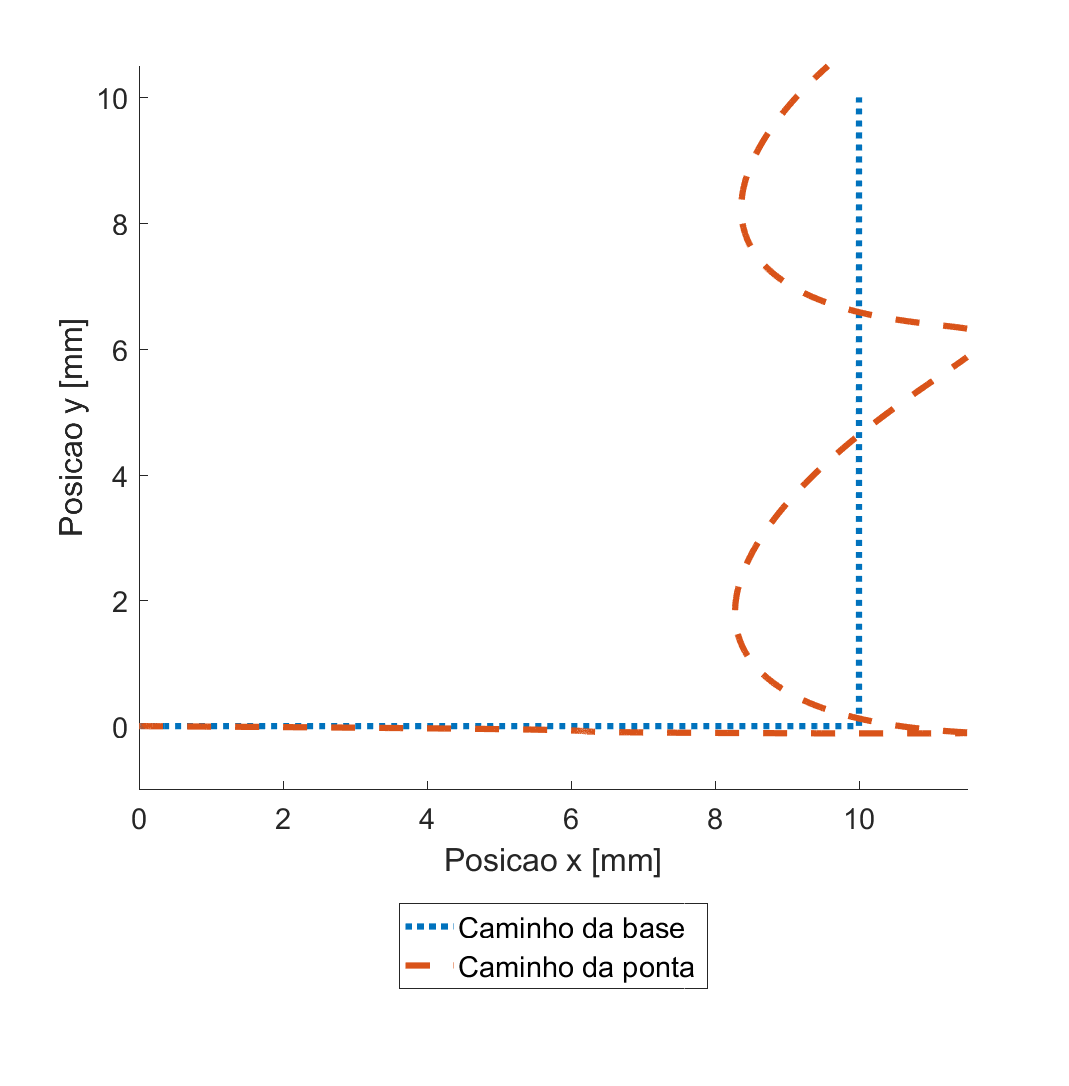
\includegraphics[width=0.47\textwidth]{Sim 2A_cam_s.png}
        \label{fig:2A_cam_s}
    }
    \hfill
    \subfigure[Com controle.]{
        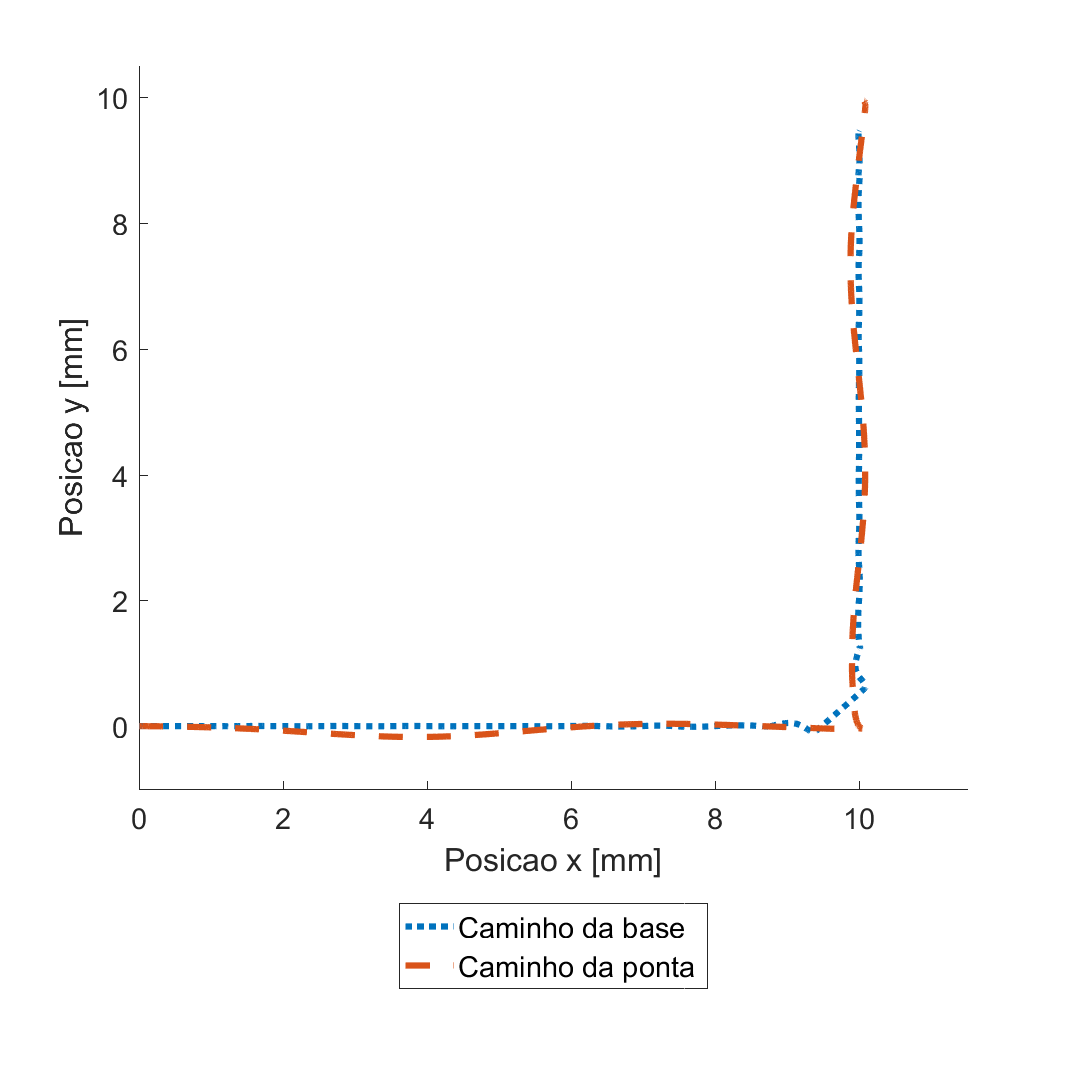
\includegraphics[width=0.47\textwidth]{Sim 2A_cam_c.png}
        \label{fig:2A_cam_c}
    }
    \hfill
    \subfigure[Detalhamento - Sem controle.]{
        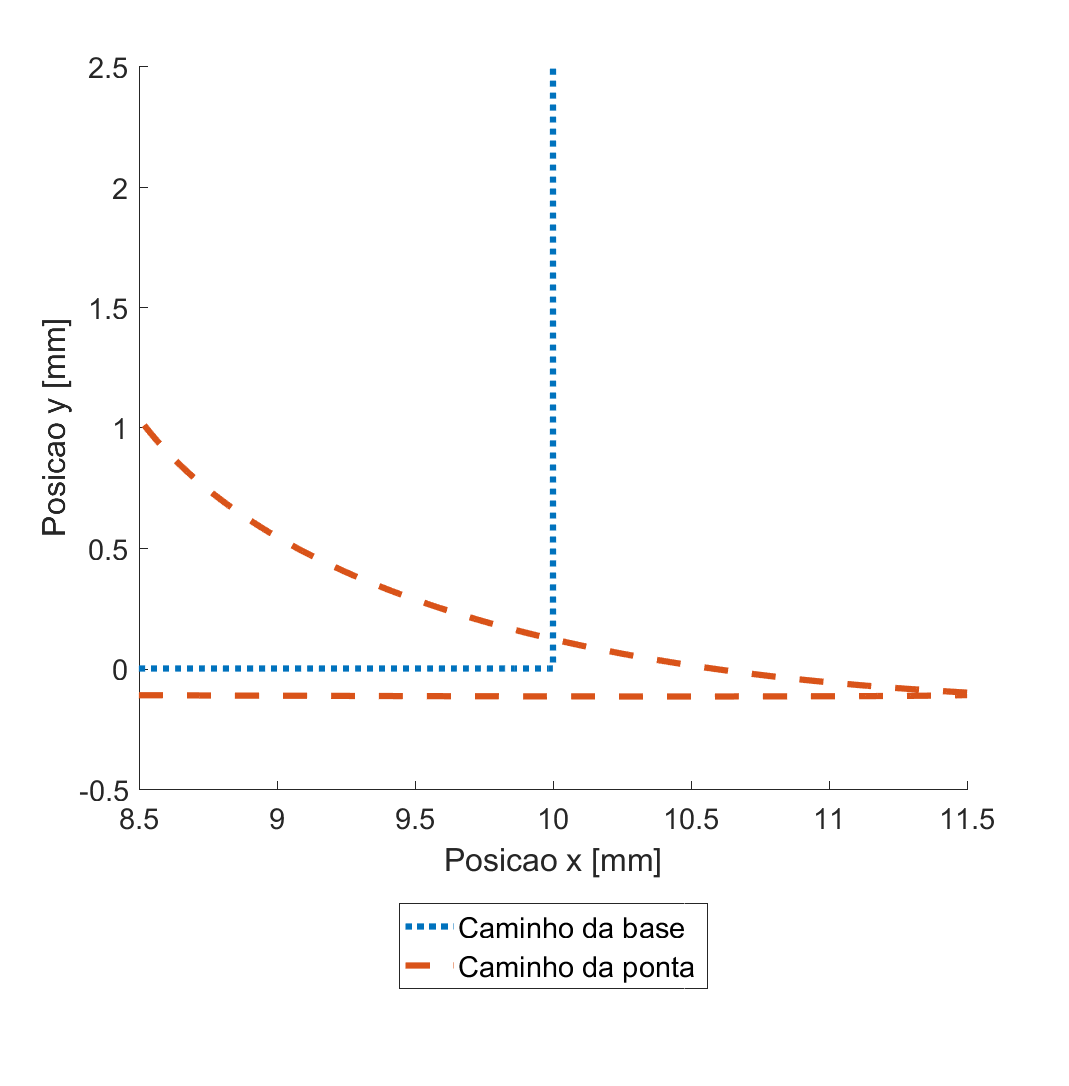
\includegraphics[width=0.47\textwidth]{Sim 2A_cam_s_zoom.png}
        \label{fig:2A_cam_s_zoom}
    }
    \hfill
    \subfigure[Detalhamento - Com controle.]{
        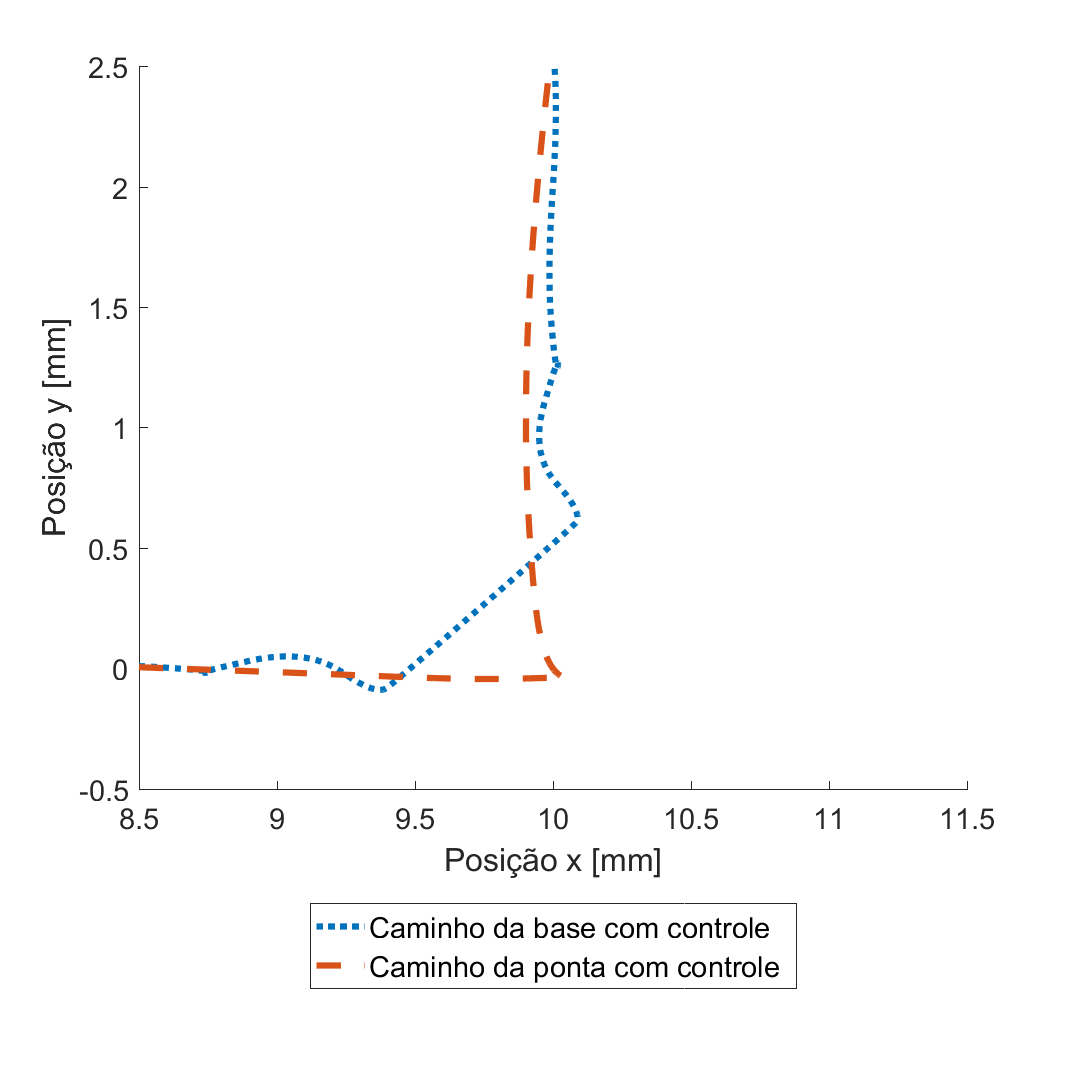
\includegraphics[width=0.47\textwidth]{Sim 2A_cam_c_zoom.png}
        \label{fig:2A_cam_c_zoom}
    }
    \caption{Caminhos da ponta e da base - Caso 2A.}
    \label{fig:2A_cam}
\end{figure}

% ------------------ Deslocamento A----------------
Na Figura \ref{fig:2A_des}, é possível confirmar as avaliações feitas no parágrafo anterior através do perfil de deslocamento com e sem controle ao longo do tempo.

% fig:des
\begin{figure}[H]
    \centering
    \subfigure[Sem controle.]{
        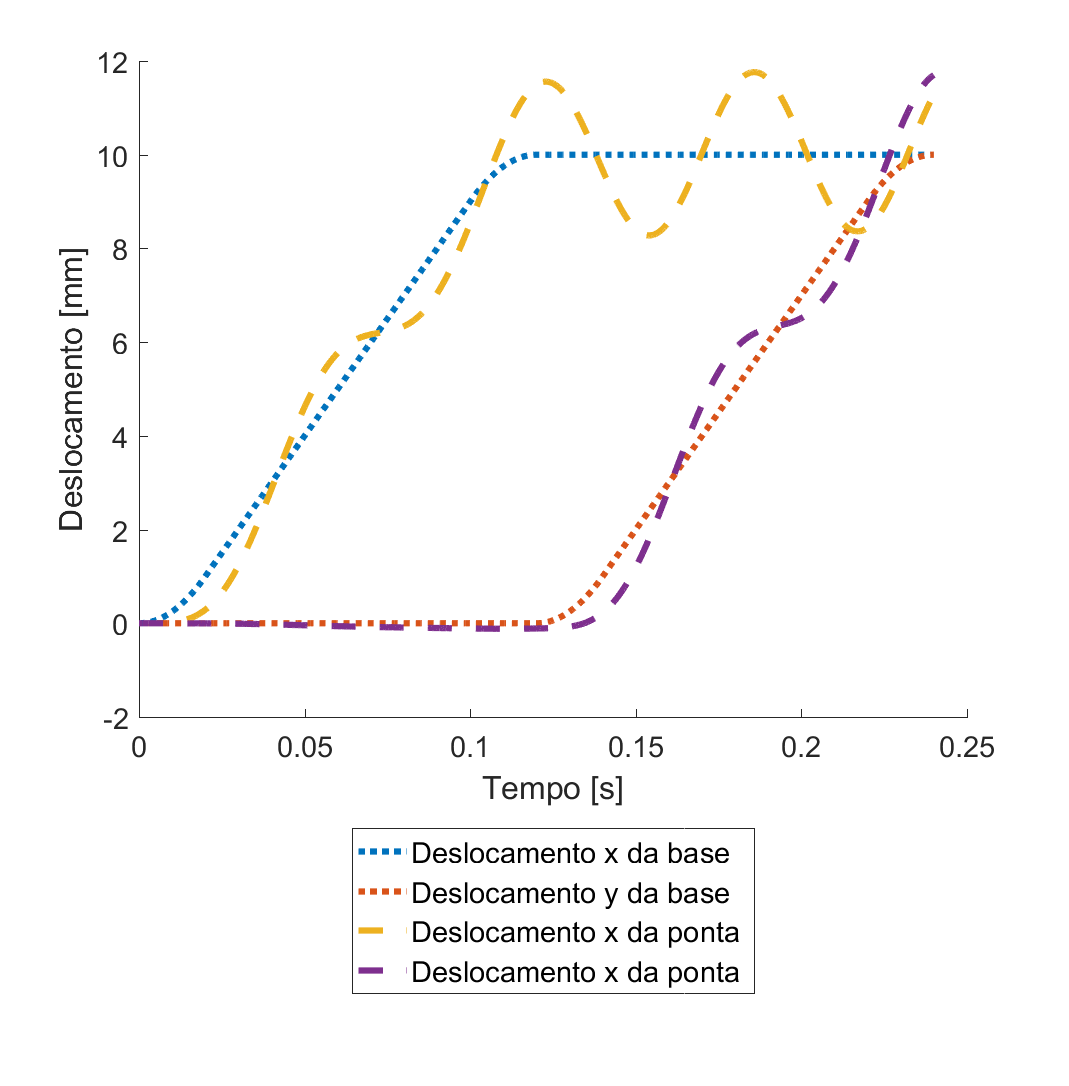
\includegraphics[width=0.47\textwidth]{Sim 2A_des_s.png}
        \label{fig:2A_des_s}
    }
    \hfill
    \subfigure[Com controle.]{
        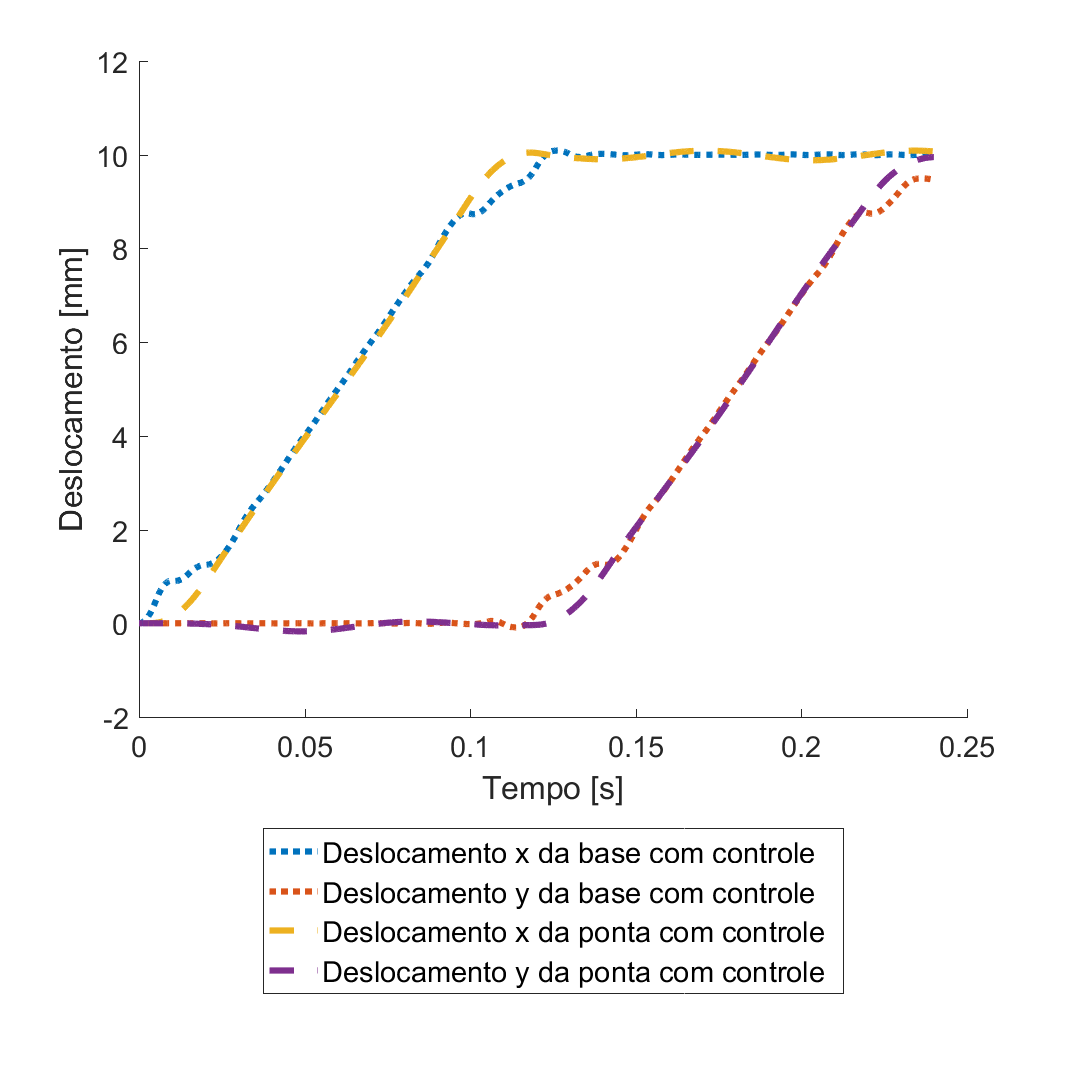
\includegraphics[width=0.47\textwidth]{Sim 2A_des_c.png}
        \label{fig:2A_des_c}
    }
    \caption{Deslocamentos da ponta e da base - Caso 2A.}
    \label{fig:2A_des}
\end{figure}

% ------------------ Velocidades A ----------------
Assim como no Caso 1A, o perfil de velocidades apresenta uma maior amplitude das oscilações. Efeito este causado pela ausência da dissipação de energia fornecida pelo sistema (coeficiente de amortecimento nulo). Além disso, o perfil de velocidades da ponta com controle se demonstra relativamente estável, apesar da necessidade de correções se manter elevado ao longo do tempo, representado pela amplitude das oscilações do perfil de velocidade da base com controle.

% fig:vel
\begin{figure}[H]
    \centering
    \subfigure[Sem controle.]{
        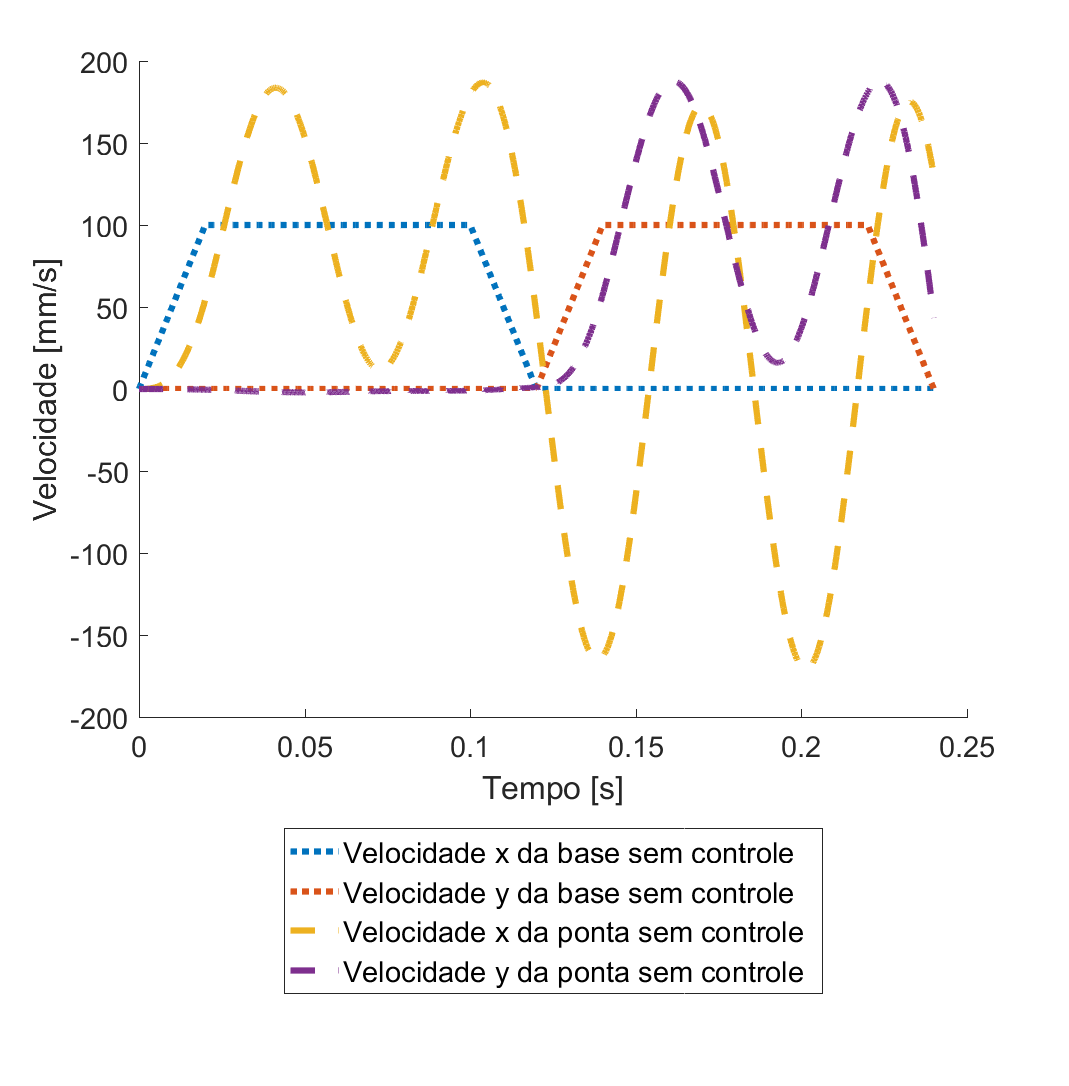
\includegraphics[width=0.47\textwidth]{Sim 2A_vel_s.png}
        \label{fig:2A_vel_s}
    }
    \hfill
    \subfigure[Com controle.]{
        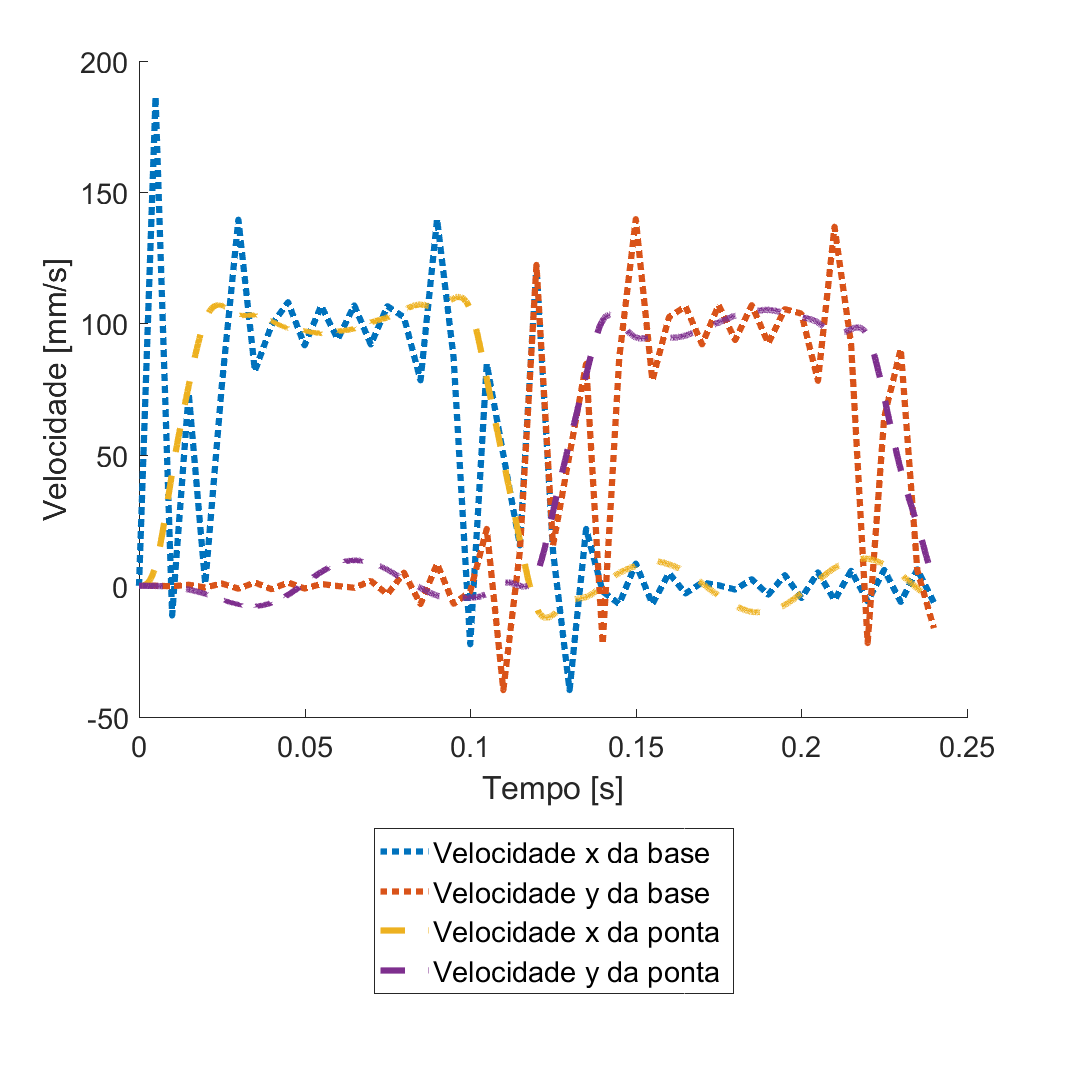
\includegraphics[width=0.47\textwidth]{Sim 2A_vel_c.png}
        \label{fig:2A_vel_c}
    }
    \caption{Velocidades da ponta e da base - Caso 2A.}
    \label{fig:2A_vel}
\end{figure}

% ------------------ Caminho B ----------------
Agora na simulação do Caso 2B (coeficiente de amortecimento \(1\)), os efeitos se assimilam ao aumento da rigidez, isto é, os desvios do caminho da ponta sem controle é reduzido assim como a intensidade da compensação fornecida pela base com controle. Efeitos esses ilustrados nas Figuras \ref{fig:2B_cam} e \ref{fig:2B_des}.

% fig:cam
\begin{figure}[H]
    \centering
    \subfigure[Sem controle.]{
        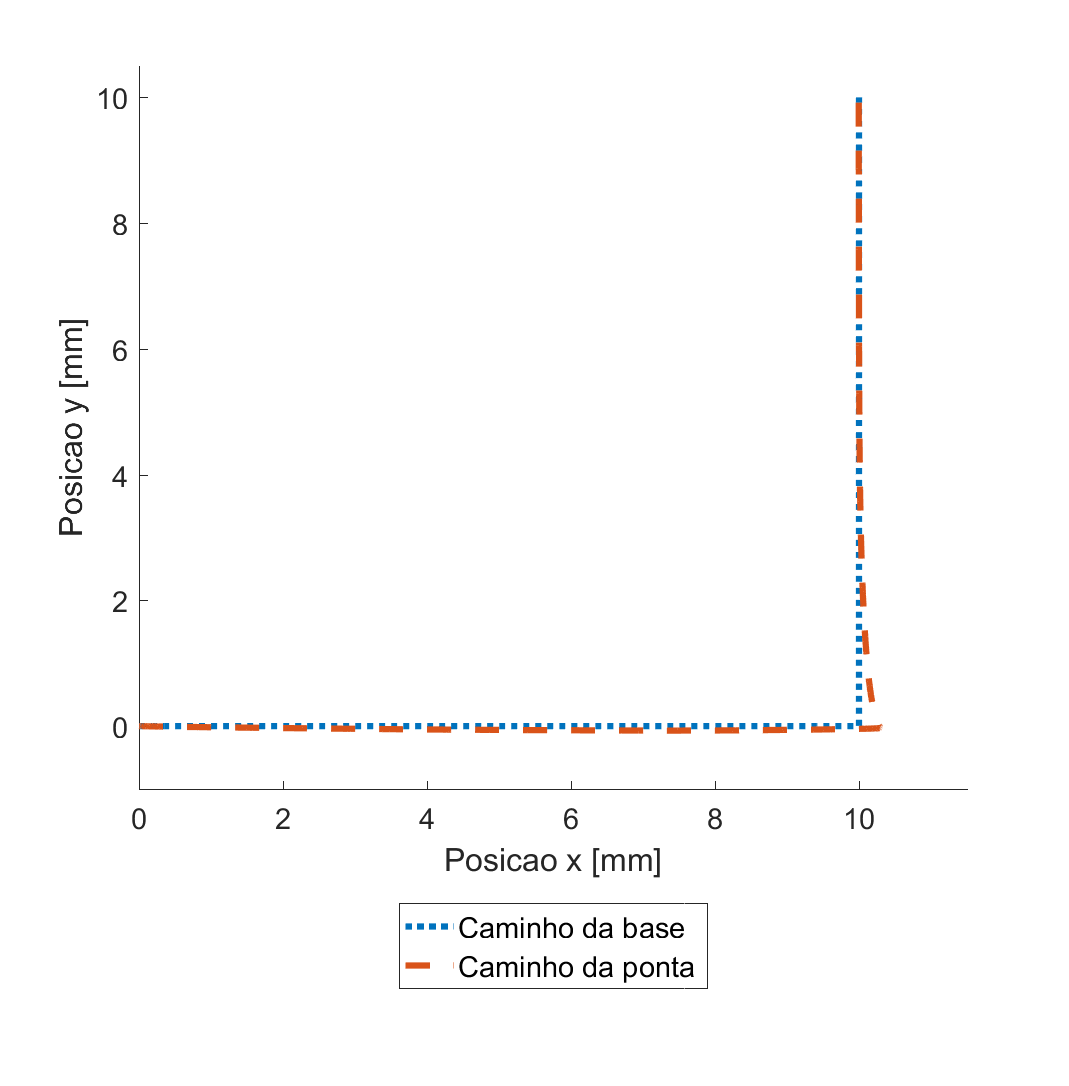
\includegraphics[width=0.47\textwidth]{Sim 2B_cam_s.png}
        \label{fig:2B_cam_s}
    }
    \hfill
    \subfigure[Com controle.]{
        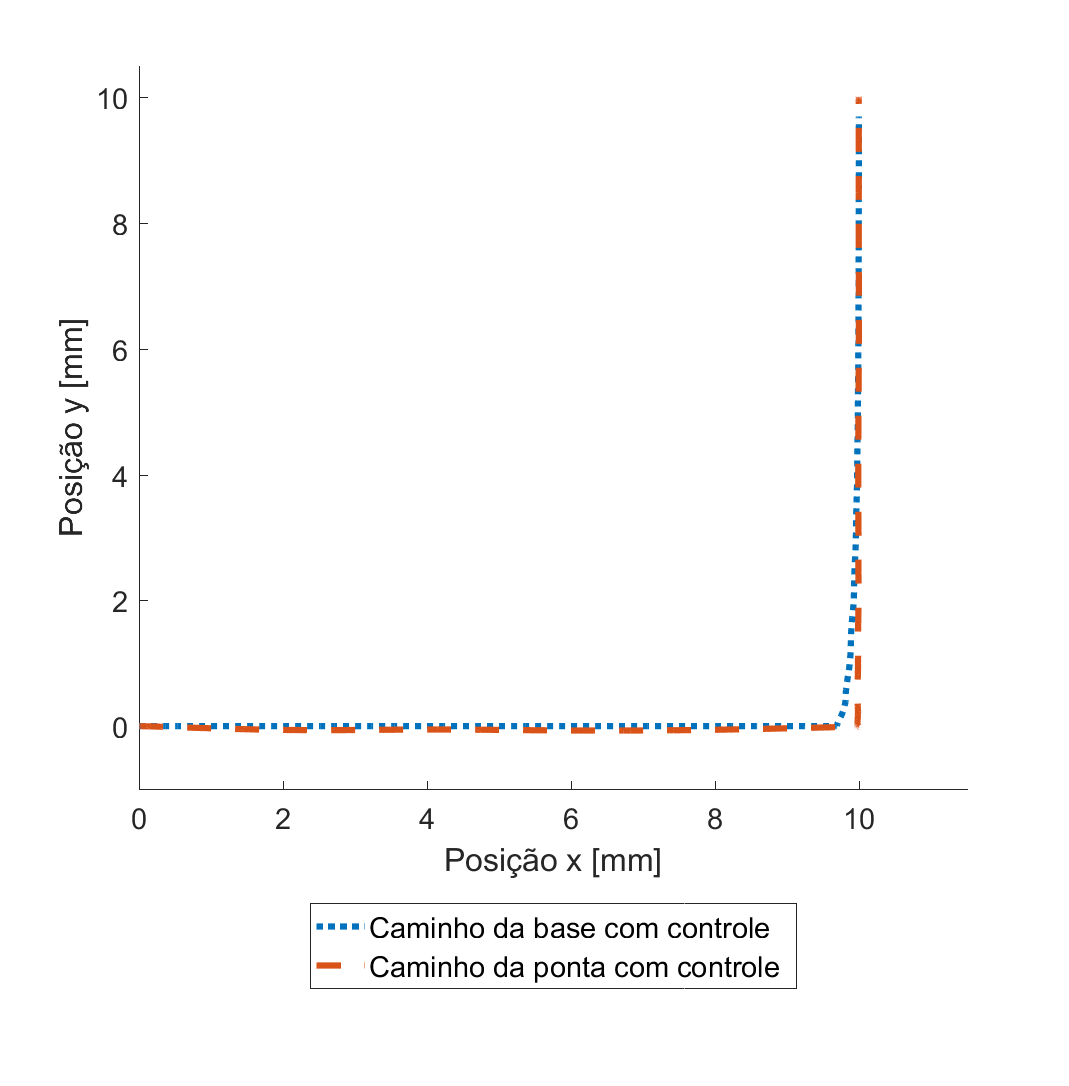
\includegraphics[width=0.47\textwidth]{Sim 2B_cam_c.png}
        \label{fig:2B_cam_c}
    }
    \hfill
    \subfigure[Detalhamento - Sem controle.]{
        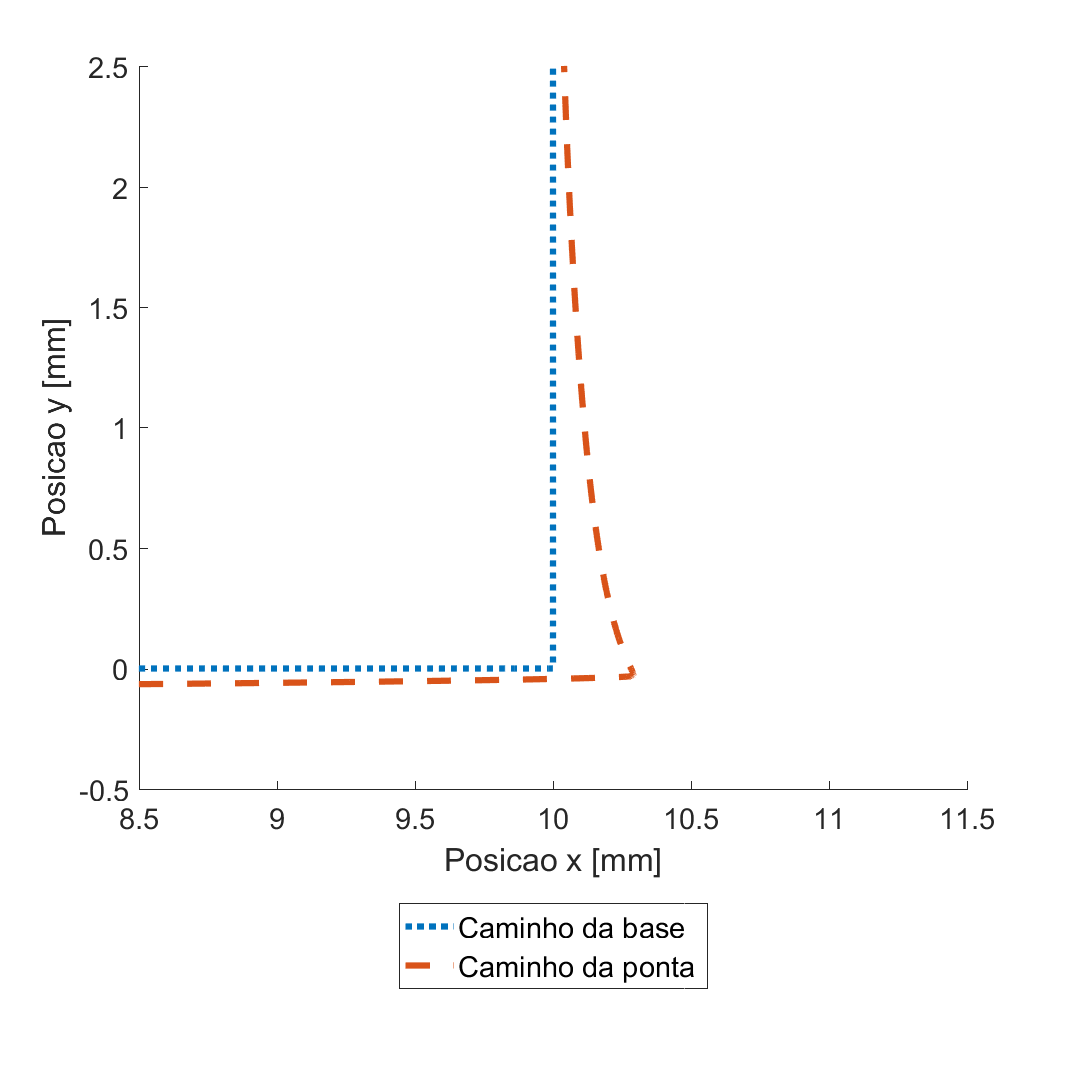
\includegraphics[width=0.47\textwidth]{Sim 2B_cam_s_zoom.png}
        \label{fig:2B_cam_s_zoom}
    }
    \hfill
    \subfigure[Detalhamento - Com controle.]{
        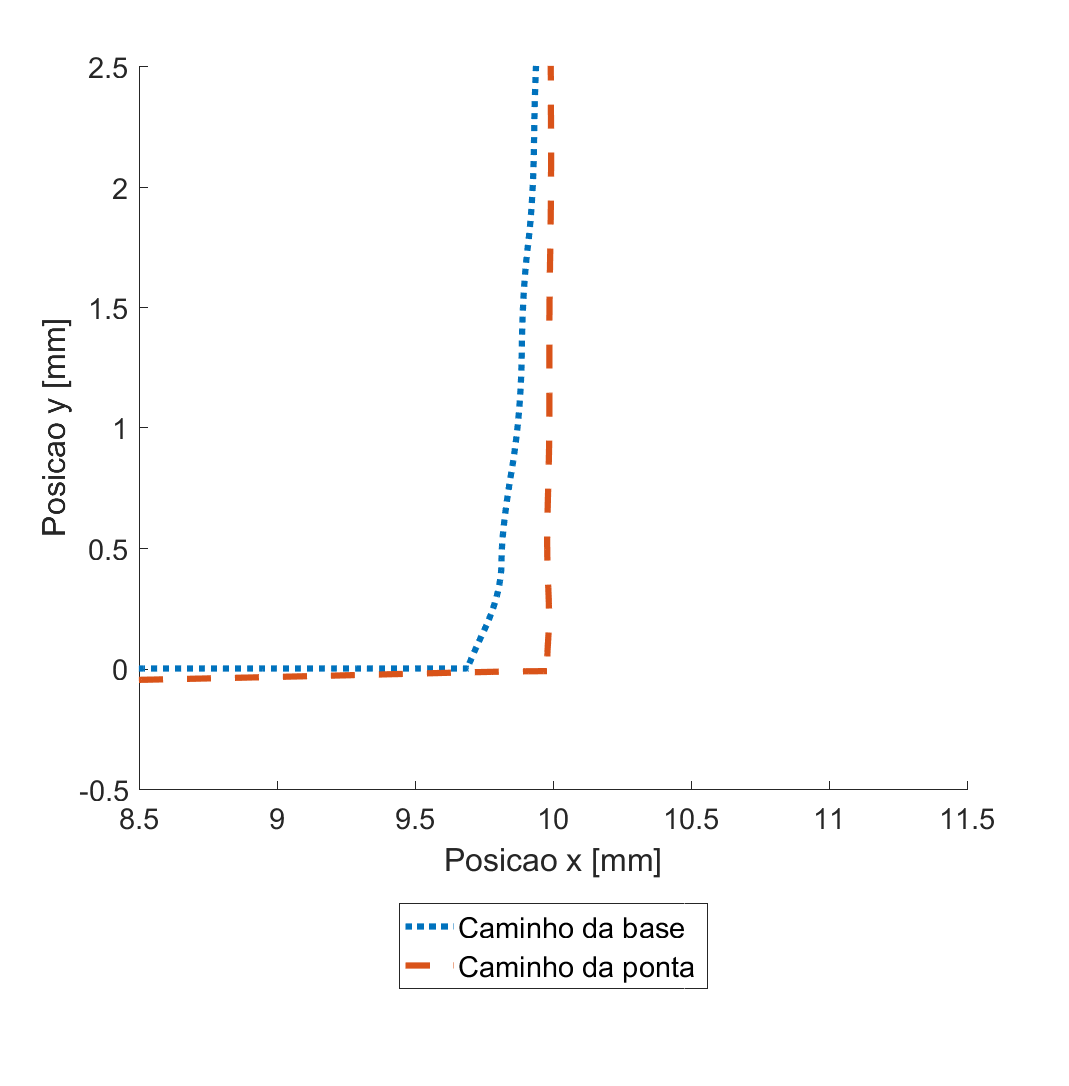
\includegraphics[width=0.47\textwidth]{Sim 2B_cam_c_zoom.png}
        \label{fig:2B_cam_c_zoom}
    }
    \caption{Caminhos da ponta e da base - Caso 2B.}
    \label{fig:2B_cam}
\end{figure}

% ------------------ Deslocamento B----------------
% fig:des
\begin{figure}[H]
    \centering
    \subfigure[Sem controle.]{
        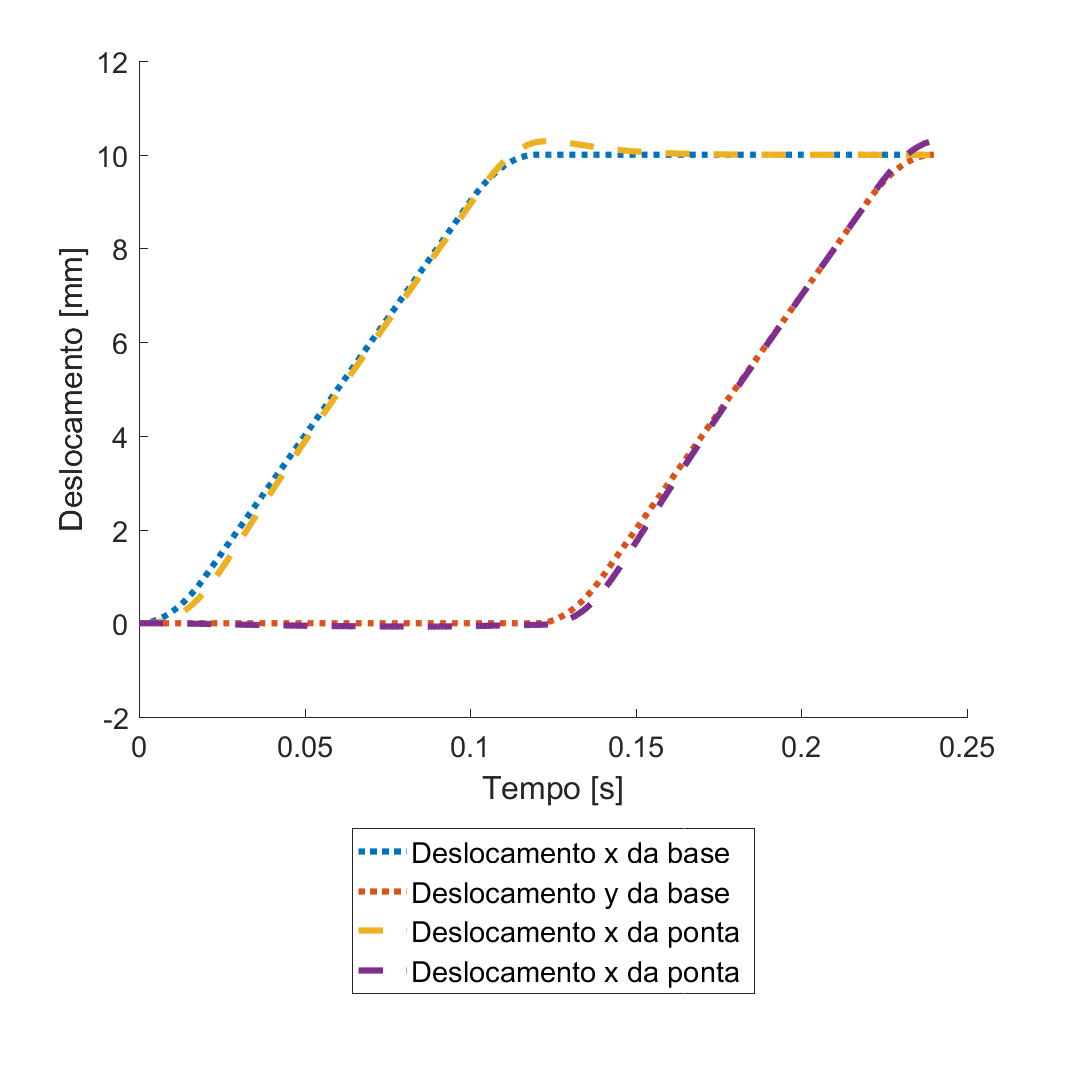
\includegraphics[width=0.47\textwidth]{Sim 2B_des_s.png}
        \label{fig:2B_des_s}
    }
    \hfill
    \subfigure[Com controle.]{
        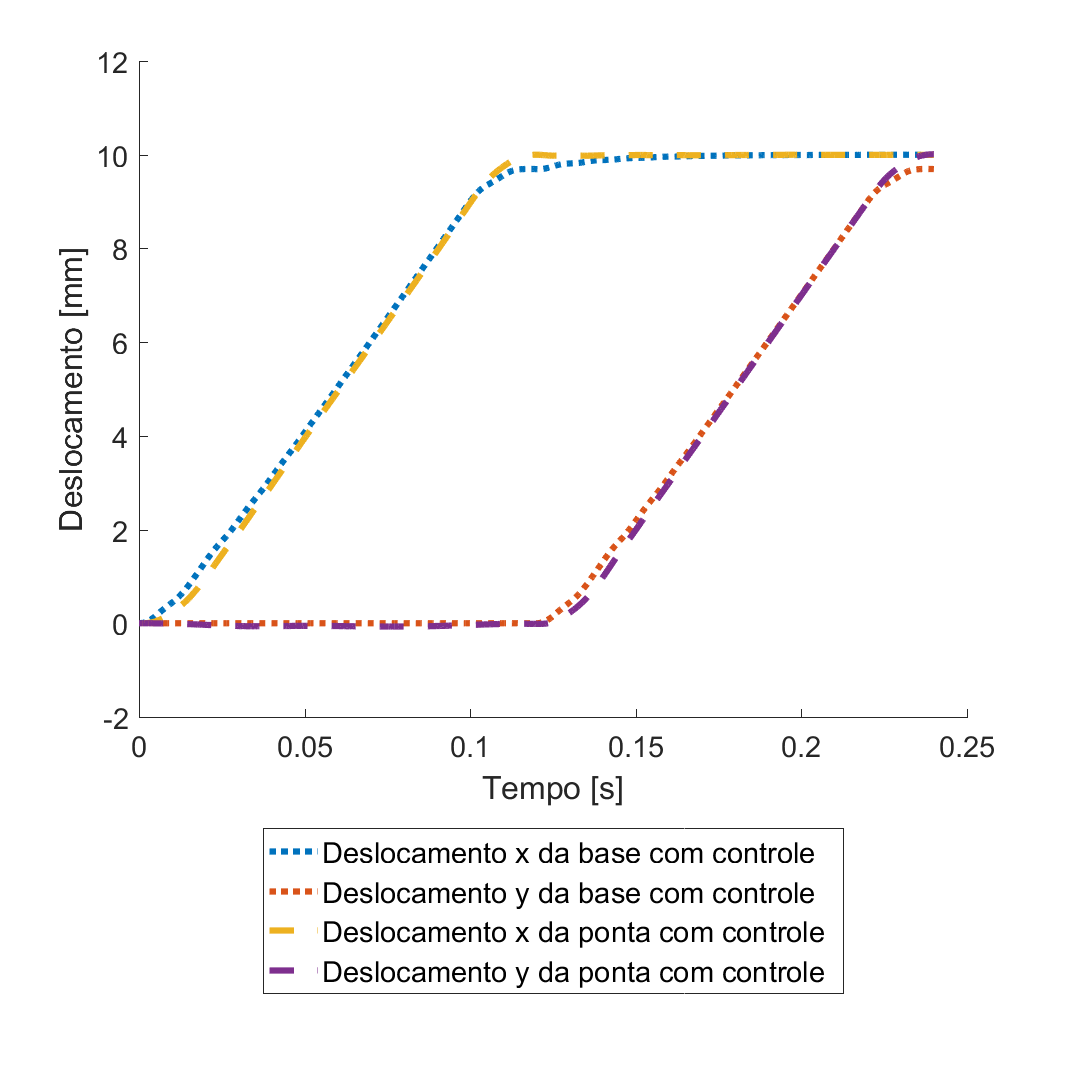
\includegraphics[width=0.47\textwidth]{Sim 2B_des_c.png}
        \label{fig:2B_des_c}
    }
    \caption{Deslocamentos da ponta e da base - Caso 2B.}
    \label{fig:2B_des}
\end{figure}

% ------------------ Velocidades B ----------------
Além disso, na Figura \ref{fig:2B_vel} observa-se o decaimento das oscilações do perfil de velocidade da base com controle de maneira mais rápida do que na simulação de referência. Fato esse que corrobora para as observações realizadas sobre o comportamento desta simulação.

% fig:vel
\begin{figure}[H]
    \centering
    \subfigure[Sem controle.]{
        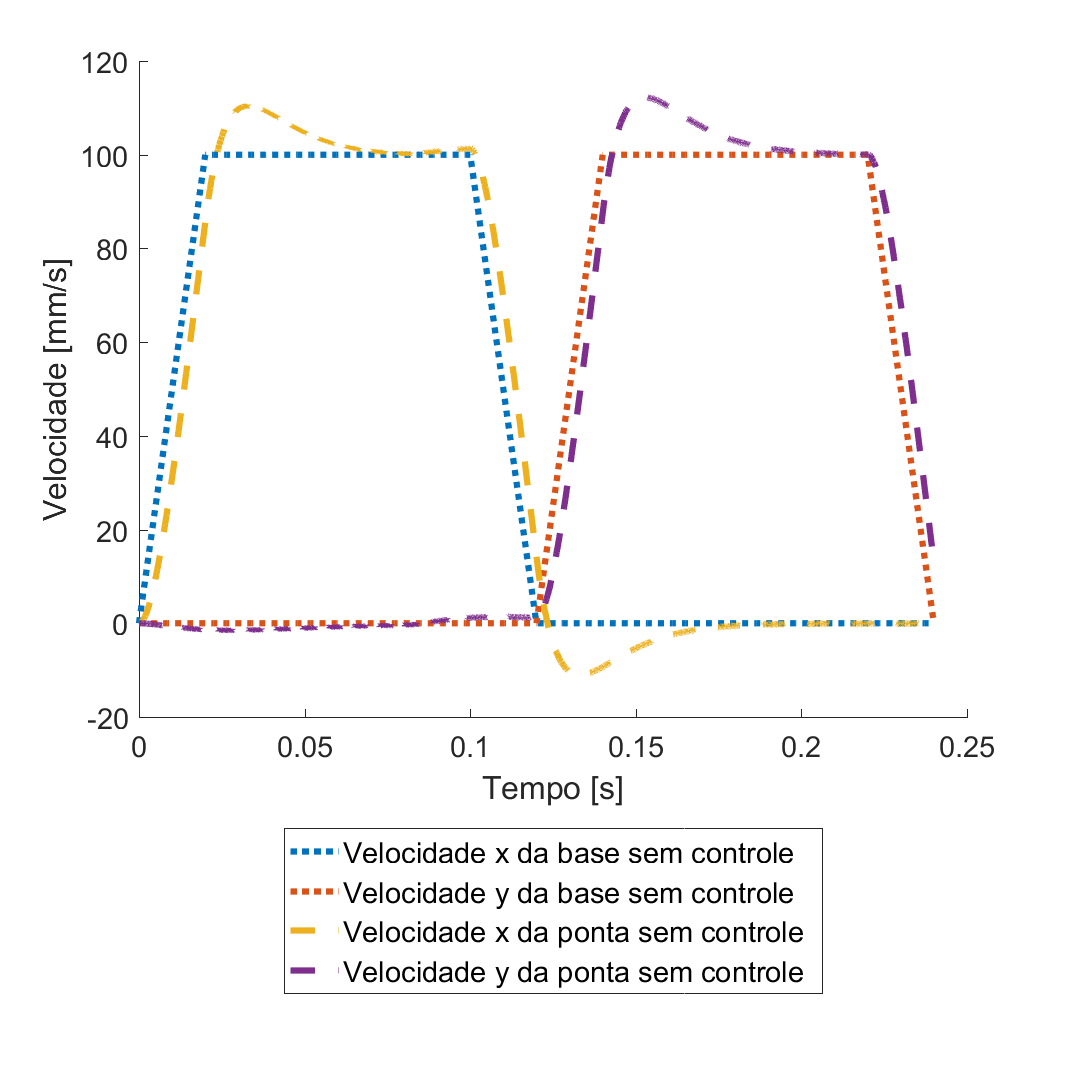
\includegraphics[width=0.47\textwidth]{Sim 2B_vel_s.png}
        \label{fig:2B_vel_s}
    }
    \hfill
    \subfigure[Com controle.]{
        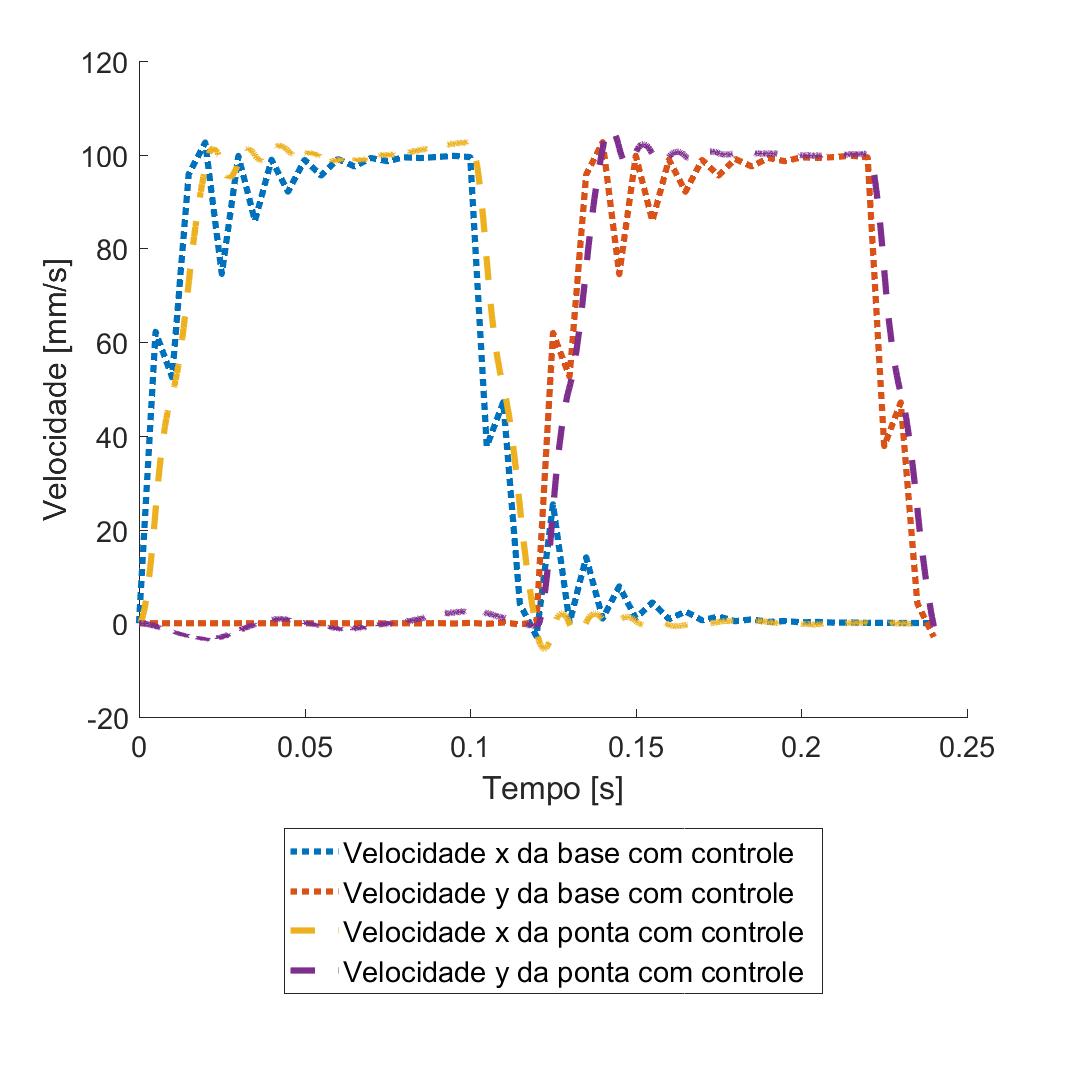
\includegraphics[width=0.47\textwidth]{Sim 2B_vel_c.png}
        \label{fig:2B_vel_c}
    }
    \caption{Velocidades da ponta e da base - Caso 2B.}
    \label{fig:2B_vel}
\end{figure}

% ------------------ end ----------------
\subsection{Caso 3 - Variação na aceleração}
Esta seção explora os efeitos da variação na aceleração sobre o comportamento dinâmico do sistema. A análise é realizada nas simulações do Caso 3A (com menor aceleração) e do Caso 3B (com maior aceleração).
% ------------------ Caminho A ----------------
Com uma aceleração mais baixa, caracterizada por forças inerciais reduzidas, observamos um comportamento mais contido no sistema. As oscilações e os desvios do caminho desejado são menores, como evidenciado na Figura \ref{fig:3A_cam} para o caminho. Enquanto as diferenças entre os caminhos com controle e sem controle mantém o mesmo comportamento apresentado na simulação de referência.

% fig:cam
\begin{figure}[H]
    \centering
    \subfigure[Sem controle.]{
        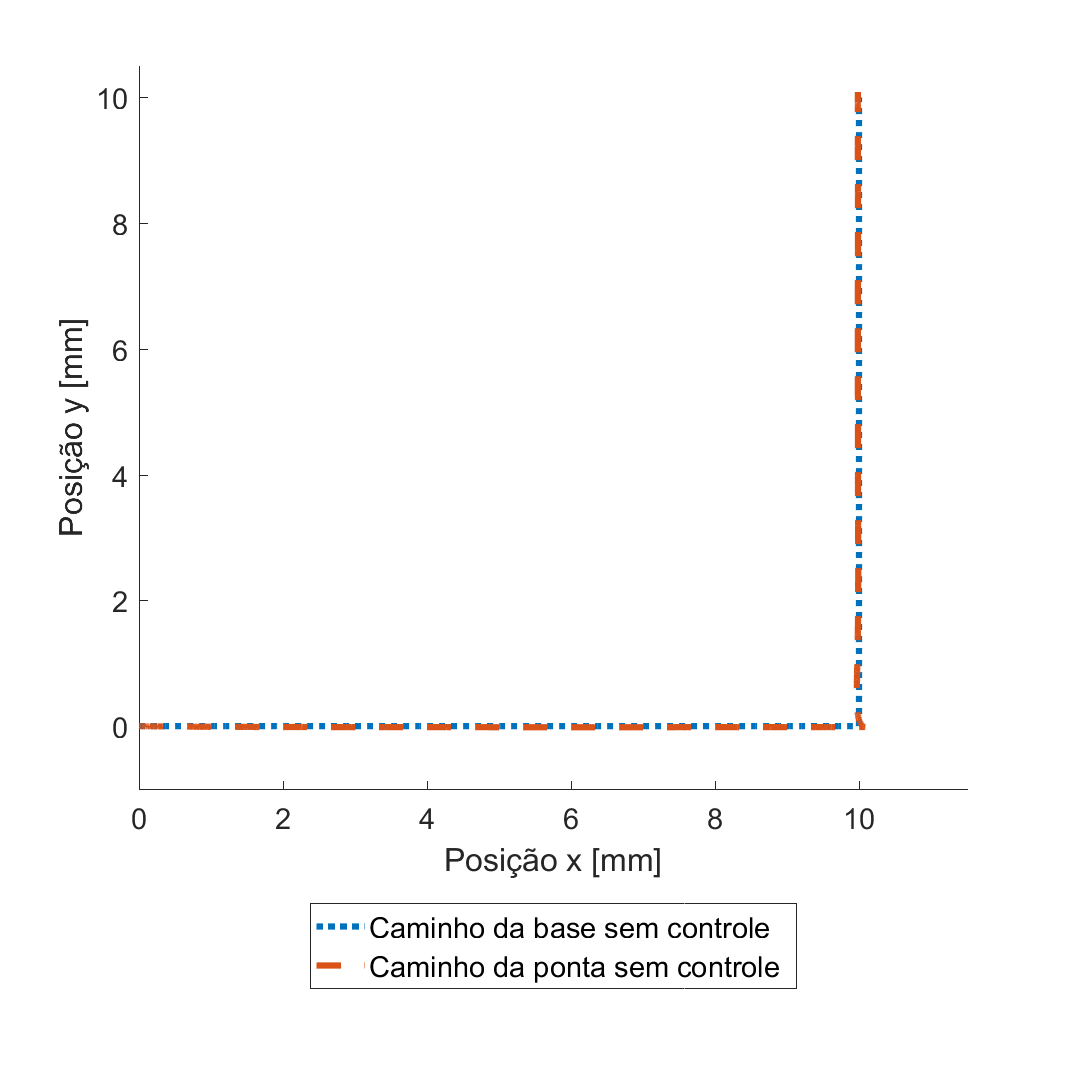
\includegraphics[width=0.47\textwidth]{Sim 3A_cam_s.png}
        \label{fig:3A_cam_s}
    }
    \hfill
    \subfigure[Com controle.]{
        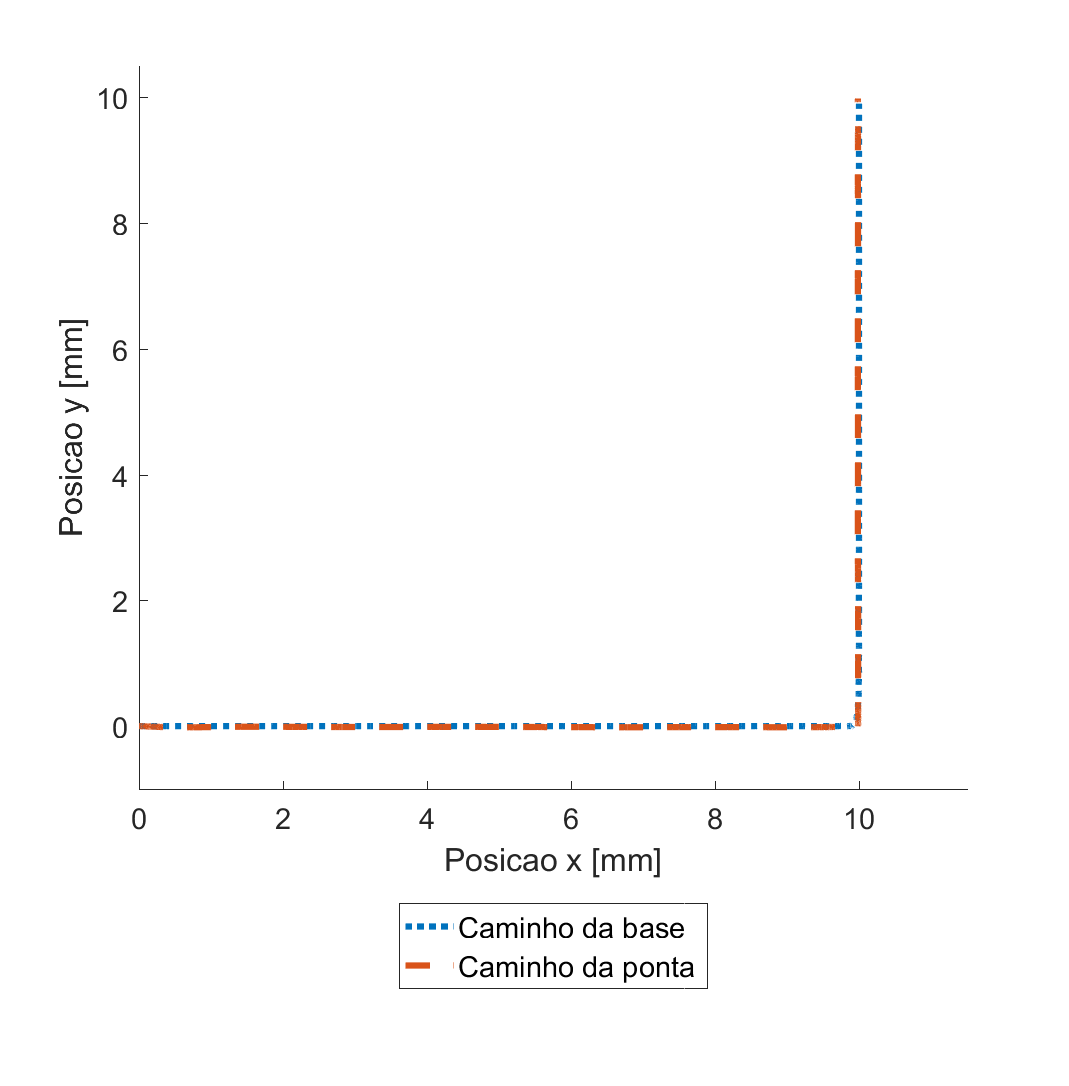
\includegraphics[width=0.47\textwidth]{Sim 3A_cam_c.png}
        \label{fig:3A_cam_c}
    }
    \hfill
    \subfigure[Detalhamento - Sem controle.]{
        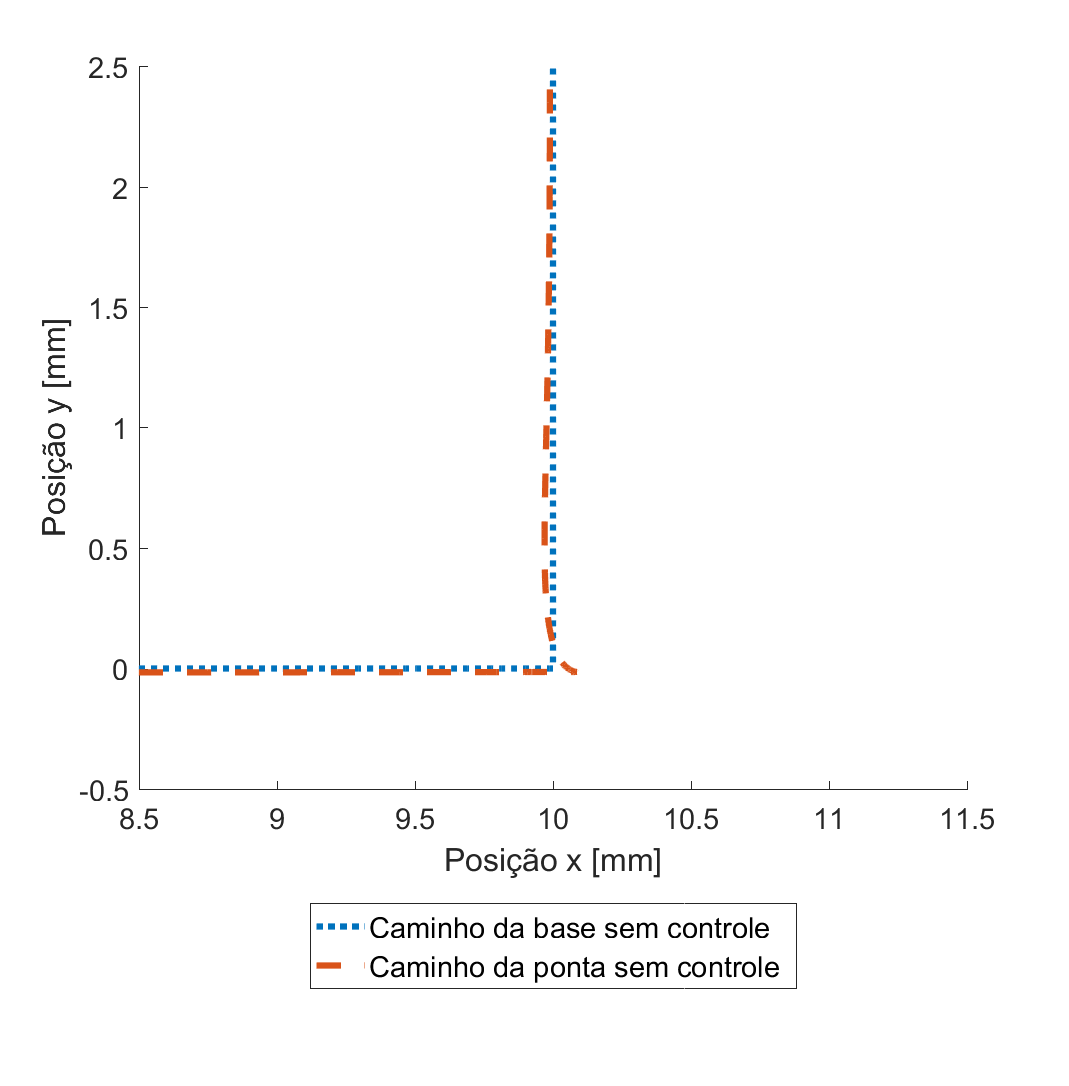
\includegraphics[width=0.47\textwidth]{Sim 3A_cam_s_zoom.png}
        \label{fig:3A_cam_s_zoom}
    }
    \hfill
    \subfigure[Detalhamento - Com controle.]{
        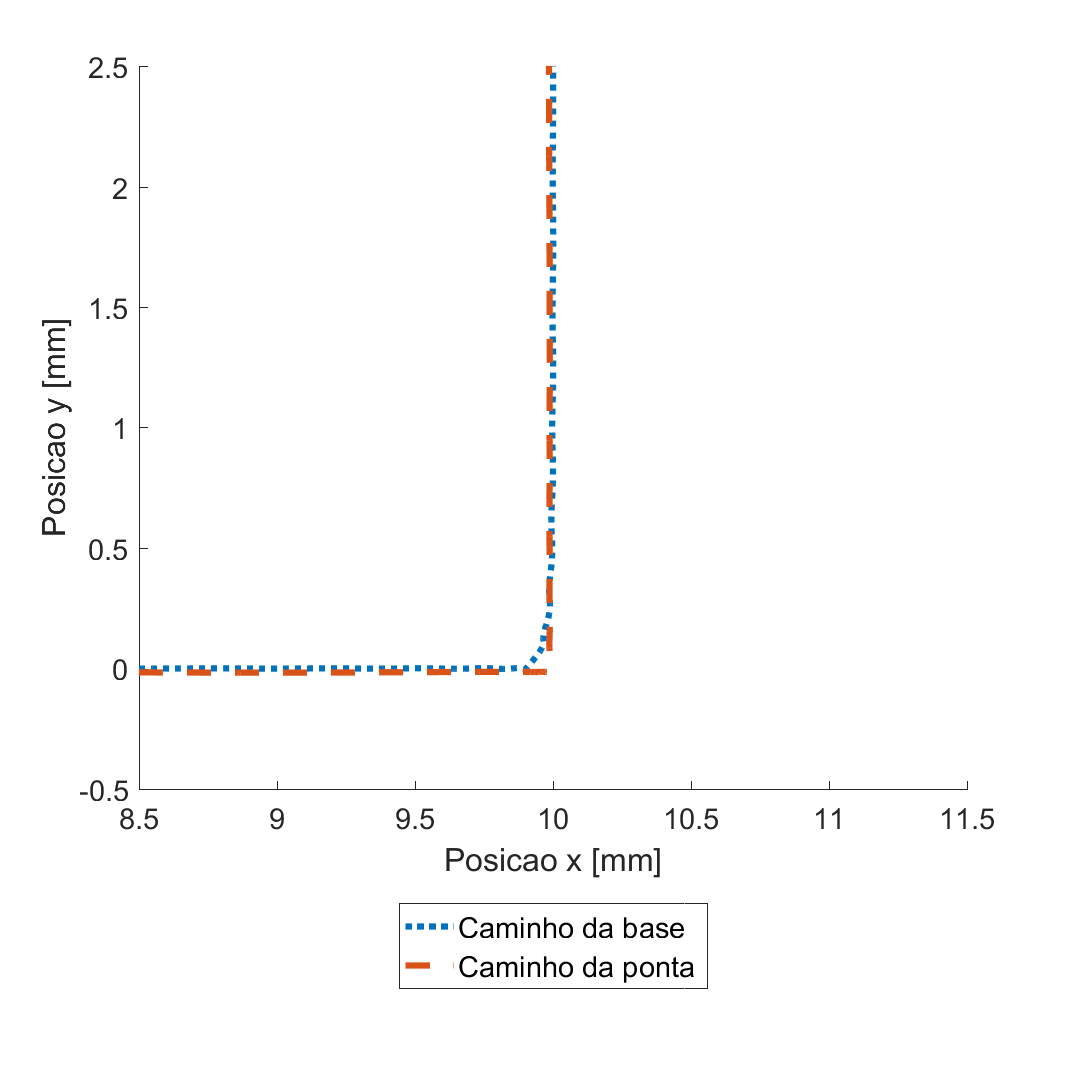
\includegraphics[width=0.47\textwidth]{Sim 3A_cam_c_zoom.png}
        \label{fig:3A_cam_c_zoom}
    }
    \caption{Caminhos da ponta e da base - Caso 3A.}
    \label{fig:3A_cam}
\end{figure}

% ------------------ Deslocamento A----------------
No gráfico de deslocamento (Figura \ref{fig:3A_des}), essa menor aceleração se traduz em uma trajetória mais suave para todas as curvas, refletindo uma menor perturbação dinâmica nas curvas da ponta.

% fig:des
\begin{figure}[H]
    \centering
    \subfigure[Sem controle.]{
        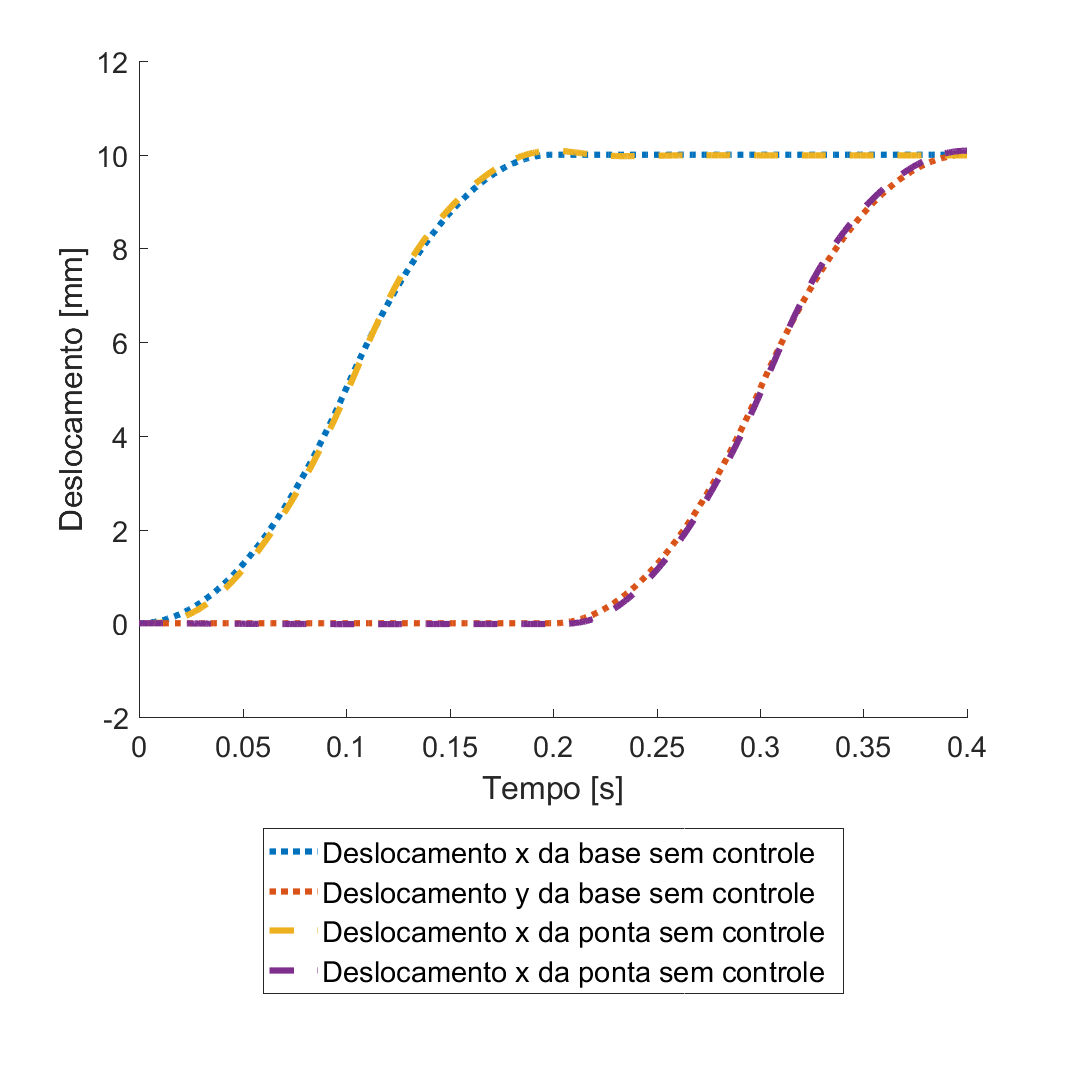
\includegraphics[width=0.47\textwidth]{Sim 3A_des_s.png}
        \label{fig:3A_des_s}
    }
    \hfill
    \subfigure[Com controle.]{
        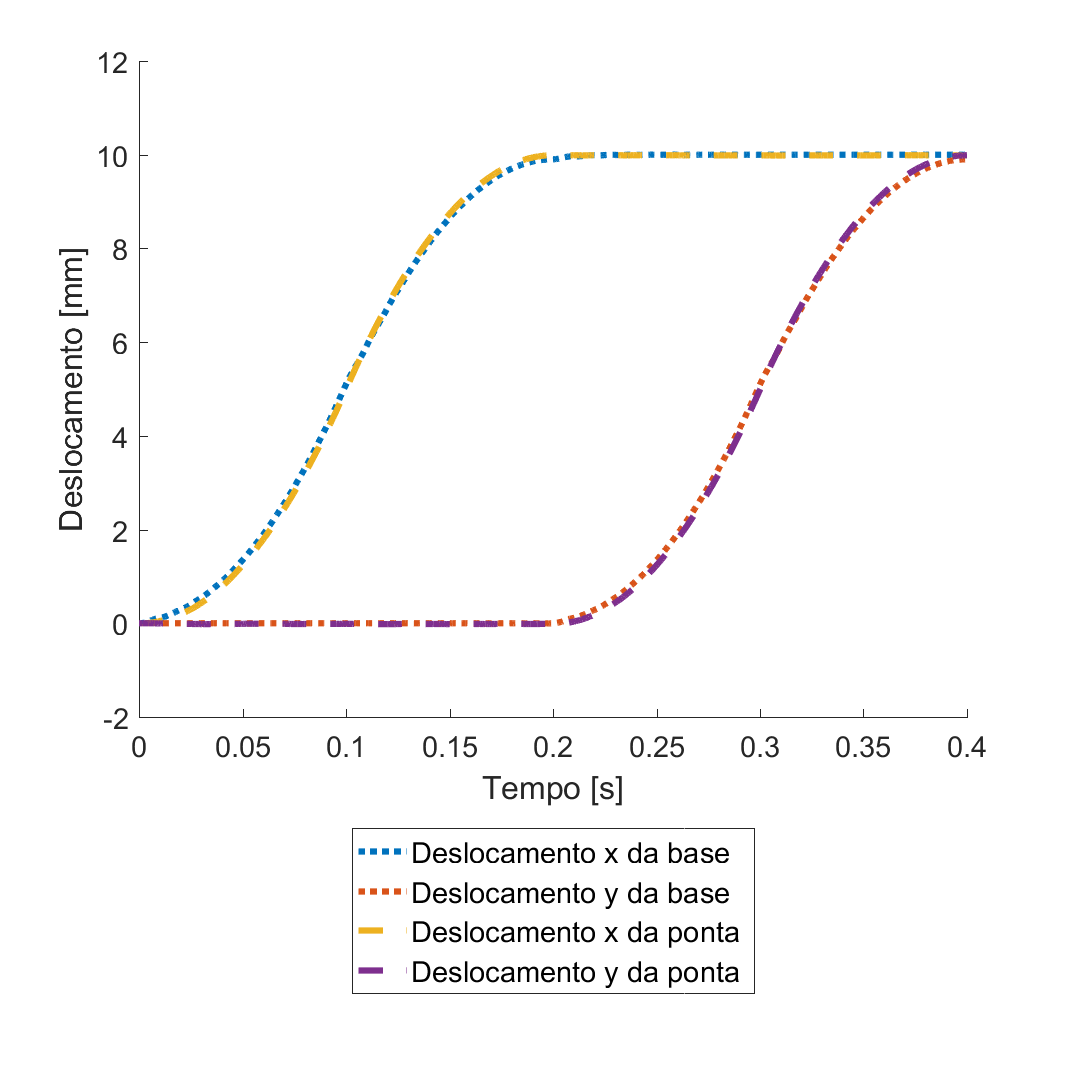
\includegraphics[width=0.47\textwidth]{Sim 3A_des_c.png}
        \label{fig:3A_des_c}
    }
    \caption{Deslocamentos da ponta e da base - Caso 3A.}
    \label{fig:3A_des}
\end{figure}

% ------------------ Velocidades A ----------------
A Figura \ref{fig:3A_vel} apresenta o perfil de velocidade para o Caso 3A, mostrando um perfil de velocidade de formato triangular e velocidade média mais baixa, consequentemente resultando em tempo de impressão mais prolongado. Além disso, apresenta também a característica oscilatória do perfil da base com controle que faz com que o perfil da ponta com controle se aproxime mais ao formato triangular visto na curva de velocidade da base sem controle.

% fig:vel
\begin{figure}[H]
    \centering
    \subfigure[Sem controle.]{
        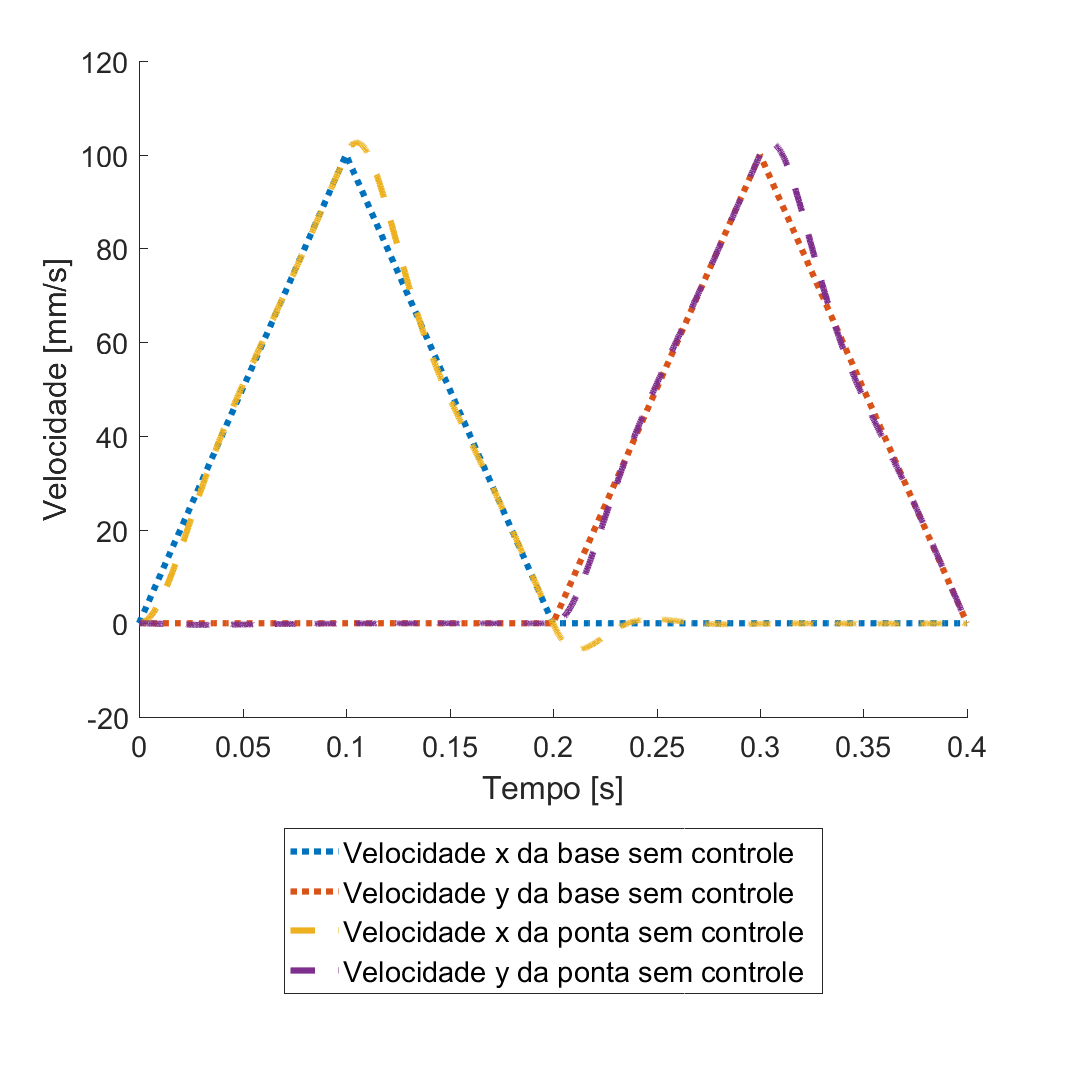
\includegraphics[width=0.47\textwidth]{Sim 3A_vel_s.png}
        \label{fig:3A_vel_s}
    }
    \hfill
    \subfigure[Com controle.]{
        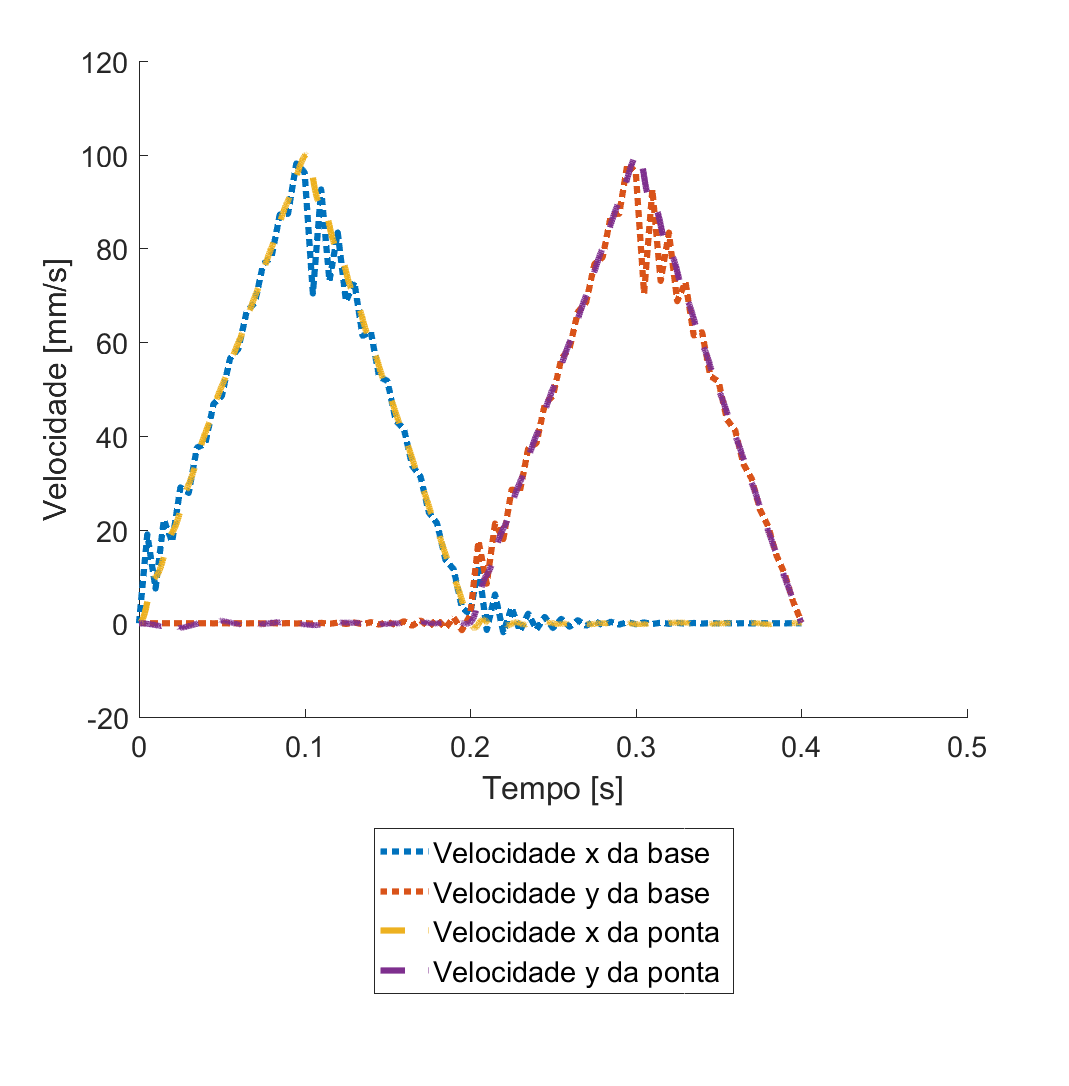
\includegraphics[width=0.47\textwidth]{Sim 3A_vel_c.png}
        \label{fig:3A_vel_c}
    }
    \caption{Velocidades da ponta e da base - Caso 3A.}
    \label{fig:3A_vel}
\end{figure}

% ------------------ Caminho B ----------------
No Caso 3B, com uma aceleração mais elevada, o sistema está sujeito a forças inerciais maiores. Isso resulta em oscilações mais acentuadas e um desvio mais significativo do caminho desejado, como ilustrado na Figura \ref{fig:3B_cam} para o caminho. Entretanto, se comparados os desvios do caminho da ponta com controle dos casos 3A e 3B nota-se pouca diferença entre eles.

% fig:cam
\begin{figure}[H]
    \centering
    \subfigure[Sem controle.]{
        \includegraphics[width=0.47\textwidth]{Sim 3B_cam_s.png}
        \label{fig:3B_cam_s}
    }
    \hfill
    \subfigure[Com controle.]{
        \includegraphics[width=0.47\textwidth]{Sim 3B_cam_c.png}
        \label{fig:3B_cam_c}
    }
    \hfill
    \subfigure[Detalhamento - Sem controle.]{
        \includegraphics[width=0.47\textwidth]{Sim 3B_cam_s_zoom.png}
        \label{fig:3B_cam_s_zoom}
    }
    \hfill
    \subfigure[Detalhamento - Com controle.]{
        \includegraphics[width=0.47\textwidth]{Sim 3B_cam_c_zoom.png}
        \label{fig:3B_cam_c_zoom}
    }
    \caption{Caminhos da ponta e da base - Caso 3B.}
    \label{fig:3B_cam}
\end{figure}

% ------------------ Deslocamento B----------------
O gráfico de deslocamento (Figura \ref{fig:3B_des}) para o Caso 3B reflete essas características, exibindo um movimento mais rápido, porém com maior perturbação na curva da ponta sem controle.

% fig:des
\begin{figure}[H]
    \centering
    \subfigure[Sem controle.]{
        \includegraphics[width=0.47\textwidth]{Sim 3B_des_s.png}
        \label{fig:3B_des_s}
    }
    \hfill
    \subfigure[Com controle.]{
        \includegraphics[width=0.47\textwidth]{Sim 3B_des_c.png}
        \label{fig:3B_des_c}
    }
    \caption{Deslocamentos da ponta e da base - Caso 3B.}
    \label{fig:3B_des}
\end{figure}

% ------------------ Velocidades B ----------------
Essa maior aceleração também produz um perfil de velocidade trapezoidal com inclinações maiores e, portanto velocidade média maior, como mostrado na Figura \ref{fig:3B_vel}, reduzindo o tempo de impressão.

% fig:vel
\begin{figure}[H]
    \centering
    \subfigure[Sem controle.]{
        \includegraphics[width=0.47\textwidth]{Sim 3B_vel_s.png}
        \label{fig:3B_vel_s}
    }
    \hfill
    \subfigure[Com controle.]{
        \includegraphics[width=0.47\textwidth]{Sim 3B_vel_c.png}
        \label{fig:3B_vel_c}
    }
    \caption{Velocidades da ponta e da base - Caso 3B.}
    \label{fig:3B_vel}
\end{figure}

Interessantemente, esta análise demonstra que o controle efetivamente minimiza os aspectos negativos da maior aceleração, permitindo que o sistema aproveite a vantagem de um menor tempo de impressão sem comprometer significativamente a precisão do caminho.

% ------------------ end ----------------

\subsection{Caso 4 - Variação da velocidade desejada}
A variação da velocidade desejada possui efeitos similares à variação da aceleração. Onde observa-se um menor desvio no caminho da ponta sem controle (Figura \ref{fig:5A_cam}) e um maior tempo de impressão, assim como uma alteração no formato do perfil de velocidade (Figuras \ref{fig:5A_des} e \ref{fig:5A_vel})

% ------------------ Caminho A ----------------
% fig:cam
\begin{figure}[H]
    \centering
    \subfigure[Sem controle.]{
        \includegraphics[width=0.47\textwidth]{Sim 5A_cam_s.png}
        \label{fig:5A_cam_s}
    }
    \hfill
    \subfigure[Com controle.]{
        \includegraphics[width=0.47\textwidth]{Sim 5A_cam_c.png}
        \label{fig:5A_cam_c}
    }
    \hfill
    \subfigure[Detalhamento - Sem controle.]{
        \includegraphics[width=0.47\textwidth]{Sim 5A_cam_s_zoom.png}
        \label{fig:5A_cam_s_zoom}
    }
    \hfill
    \subfigure[Detalhamento - Com controle.]{
        \includegraphics[width=0.47\textwidth]{Sim 5A_cam_c_zoom.png}
        \label{fig:5A_cam_c_zoom}
    }
    \caption{Caminhos da ponta e da base - Caso 4A.}
    \label{fig:5A_cam}
\end{figure}

% ------------------ Deslocamento A----------------
% fig:des
\begin{figure}[H]
    \centering
    \subfigure[Sem controle.]{
        \includegraphics[width=0.47\textwidth]{Sim 5A_des_s.png}
        \label{fig:5A_des_s}
    }
    \hfill
    \subfigure[Com controle.]{
        \includegraphics[width=0.47\textwidth]{Sim 5A_des_c.png}
        \label{fig:5A_des_c}
    }
    \caption{Deslocamentos da ponta e da base - Caso 4A.}
    \label{fig:5A_des}
\end{figure}

% ------------------ Velocidades A ----------------
% fig:vel
\begin{figure}[H]
    \centering
    \subfigure[Sem controle.]{
        \includegraphics[width=0.47\textwidth]{Sim 5A_vel_s.png}
        \label{fig:5A_vel_s}
    }
    \hfill
    \subfigure[Com controle.]{
        \includegraphics[width=0.47\textwidth]{Sim 5A_vel_c.png}
        \label{fig:5A_vel_c}
    }
    \caption{Velocidades da ponta e da base - Caso 4A.}
    \label{fig:5A_vel}
\end{figure}

% ------------------ Caminho B ----------------
As características do maior desvio do caminho da ponta sem controle, assim como o desvio semelhante do caminho da ponta com controle se mantém similares às vistas na variação da aceleração.
Este comportamento é ilustrado na Figura \ref{fig:5B_cam}.

% fig:cam
\begin{figure}[H]
    \centering
    \subfigure[Sem controle.]{
        \includegraphics[width=0.47\textwidth]{Sim 5B_cam_s.png}
        \label{fig:5B_cam_s}
    }
    \hfill
    \subfigure[Com controle.]{
        \includegraphics[width=0.47\textwidth]{Sim 5B_cam_c.png}
        \label{fig:5B_cam_c}
    }
    \hfill
    \subfigure[Detalhamento - Sem controle.]{
        \includegraphics[width=0.47\textwidth]{Sim 5B_cam_s_zoom.png}
        \label{fig:5B_cam_s_zoom}
    }
    \hfill
    \subfigure[Detalhamento - Com controle.]{
        \includegraphics[width=0.47\textwidth]{Sim 5B_cam_c_zoom.png}
        \label{fig:5B_cam_c_zoom}
    }
    \caption{Caminhos da ponta e da base - Caso 4B.}
    \label{fig:5B_cam}
\end{figure}
% ------------------ Deslocamento B----------------
Além disso, nota-se o menor tempo de impressão através dos eixos de tempo das Figuras \ref{fig:5B_des} e \ref{fig:5B_vel} quando comparados às simulações de referência e a simulação do Caso 4A, assim como na mudança do perfil de velocidades. Mudanças essas também similares às mudanças vistas na variação da aceleração.

% fig:des
\begin{figure}[H]
    \centering
    \subfigure[Sem controle.]{
        \includegraphics[width=0.47\textwidth]{Sim 5B_des_s.png}
        \label{fig:5B_des_s}
    }
    \hfill
    \subfigure[Com controle.]{
        \includegraphics[width=0.47\textwidth]{Sim 5B_des_c.png}
        \label{fig:5B_des_c}
    }
    \caption{Deslocamentos da ponta e da base - Caso 4B.}
    \label{fig:5B_des}
\end{figure}

% ------------------ Velocidades B ----------------

% fig:vel
\begin{figure}[H]
    \centering
    \subfigure[Sem controle.]{
        \includegraphics[width=0.47\textwidth]{Sim 5B_vel_s.png}
        \label{fig:5B_vel_s}
    }
    \hfill
    \subfigure[Com controle.]{
        \includegraphics[width=0.47\textwidth]{Sim 5B_vel_c.png}
        \label{fig:5B_vel_c}
    }
    \caption{Velocidades da ponta e da base - Caso 4B.}
    \label{fig:5B_vel}
\end{figure}
% ------------------ end ----------------

\subsection{Caso 5 - Variação dos passos de tempo}

A variação dos passos de tempo utilizados na interpolação da trajetória gerada na etapa de controle de trajetória possui um impacto significativo nas características numéricas do método de controle. Este efeito é evidenciado pela comparação dos resultados entre o Caso 5A e o Caso 5B, com seus respectivos passos de tempo \(0,01\) e \(0,0001\).

No Caso 5B, observamos um tempo de simulação consideravelmente mais longo, chegando a 93 segundos. Este aumento substancial no tempo de simulação contrasta fortemente com o Caso 5A, onde o tempo de simulação foi inferior a 0,5 segundos. Esta diferença é atribuída ao passo de tempo mais fino utilizado no Caso 5B, que, embora aumente o tempo de processamento, oferece uma precisão notavelmente maior nos resultados da simulação.

% ------------------ Caminhos ----------------
A precisão aprimorada é particularmente notável no caminho da ponta com controle no Caso 5B (Figura \ref{fig:4B_cam}), onde se observa uma aderência significativamente mais próxima ao caminho desejado quando comparado com o Caso 5A (Figura \ref{fig:4A_cam}). Esta melhoria na precisão indica a eficácia de um passo de tempo mais detalhado na representação mais fiel das dinâmicas do sistema controlado.

% fig:cama
\begin{figure}[H]
    \centering
    \subfigure[Sem controle.]{
        \includegraphics[width=0.47\textwidth]{Sim 4A_cam_s.png}
        \label{fig:4A_cam_s}
    }
    \hfill
    \subfigure[Com controle.]{
        \includegraphics[width=0.47\textwidth]{Sim 4A_cam_c.png}
        \label{fig:4A_cam_c}
    }
    \hfill
    \subfigure[Detalhamento - Sem controle.]{
        \includegraphics[width=0.47\textwidth]{Sim 4A_cam_s_zoom.png}
        \label{fig:4A_cam_s_zoom}
    }
    \hfill
    \subfigure[Detalhamento - Com controle.]{
        \includegraphics[width=0.47\textwidth]{Sim 4A_cam_c_zoom.png}
        \label{fig:4A_cam_c_zoom}
    }
    \caption{Caminhos da ponta e da base - Caso 5A.}
    \label{fig:4A_cam}
\end{figure}

% fig:camb
\begin{figure}[H]
    \centering
    \subfigure[Sem controle.]{
        \includegraphics[width=0.47\textwidth]{Sim 4B_cam_s.png}
        \label{fig:4B_cam_s}
    }
    \hfill
    \subfigure[Com controle.]{
        \includegraphics[width=0.47\textwidth]{Sim 4B_cam_c.png}
        \label{fig:4B_cam_c}
    }
    \hfill
    \subfigure[Detalhamento - Sem controle.]{
        \includegraphics[width=0.47\textwidth]{Sim 4B_cam_s_zoom.png}
        \label{fig:4B_cam_s_zoom}
    }
    \hfill
    \subfigure[Detalhamento - Com controle.]{
        \includegraphics[width=0.47\textwidth]{Sim 4B_cam_c_zoom.png}
        \label{fig:4B_cam_c_zoom}
    }
    \caption{Caminhos da ponta e da base - Caso 5B.}
    \label{fig:4B_cam}
\end{figure}

% ------------------ Deslocamentos ----------------
Já nos gráficos que representam as curvas de deslocamento no tempo, Figuras \ref{fig:4A_des} e \ref{fig:4B_des}, é difícil identificar diferenças significativas.

% fig:desa
\begin{figure}[H]
    \centering
    \subfigure[Sem controle.]{
        \includegraphics[width=0.47\textwidth]{Sim 4A_des_s.png}
        \label{fig:4A_des_s}
    }
    \hfill
    \subfigure[Com controle.]{
        \includegraphics[width=0.47\textwidth]{Sim 4A_des_c.png}
        \label{fig:4A_des_c}
    }
    \caption{Deslocamentos da ponta e da base - Caso 5A.}
    \label{fig:4A_des}
\end{figure}

% fig:desb
\begin{figure}[H]
    \centering
    \subfigure[Sem controle.]{
        \includegraphics[width=0.47\textwidth]{Sim 4B_des_s.png}
        \label{fig:4B_des_s}
    }
    \hfill
    \subfigure[Com controle.]{
        \includegraphics[width=0.47\textwidth]{Sim 4B_des_c.png}
        \label{fig:4B_des_c}
    }
    \caption{Deslocamentos da ponta e da base - Caso 5B.}
    \label{fig:4B_des}
\end{figure}
% ------------------ Velocidades A ----------------
Além disso, o perfil de velocidade no Caso 5B (Figura \ref{fig:4B_vel}) destaca-se por sua clareza e definição, em contraste com o perfil serrilhado observado no Caso 5A (Figura \ref{fig:4A_vel}) e na simulação de referência (Figura \ref{fig:ref_vel}). Esta característica do perfil de velocidade no Caso 5B reflete uma representação mais precisa da dinâmica do sistema, evidenciando o valor de um passo de tempo mais refinado para a precisão geral da simulação.

% fig:vela
\begin{figure}[H]
    \centering
    \subfigure[Sem controle.]{
        \includegraphics[width=0.47\textwidth]{Sim 4A_vel_s.png}
        \label{fig:4A_vel_s}
    }
    \hfill
    \subfigure[Com controle.]{
        \includegraphics[width=0.47\textwidth]{Sim 4A_vel_c.png}
        \label{fig:4A_vel_c}
    }
    \caption{Velocidades da ponta e da base - Caso 5A.}
    \label{fig:4A_vel}
\end{figure}

% fig:velb
\begin{figure}[H]
    \centering
    \subfigure[Sem controle.]{
        \includegraphics[width=0.47\textwidth]{Sim 4B_vel_s.png}
        \label{fig:4B_vel_s}
    }
    \hfill
    \subfigure[Com controle.]{
        \includegraphics[width=0.47\textwidth]{Sim 4B_vel_c.png}
        \label{fig:4B_vel_c}
    }
    \caption{Velocidades da ponta e da base - Caso 5B.}
    \label{fig:4B_vel}
\end{figure}
% ------------------ end ----------------

\section{Discussão Integrada dos Resultados}
Realizadas as simulações com a variação dos parâmetros do método proposto no presente trabalho, ressalta-se a relação entre a frequência natural e o passo de tempo. Tal relação é muitas vezes discutida na literatura, se tratando de amostragem de sinais. É observado nestes resultados também, a relação entre a precisão alcançada e a proporcionalidade entre o passo de tempo e a frequência natural. Essa característica vem a tona ao se analisar o intervalo de tempo entre as oscilações e o passo de tempo. Onde um passo de tempo maior do que o período de oscilação, resulta em uma perda grande de informação e compromete a representatividade da curva discretizada. Sendo ideal um ajuste do passo de tempo dada a frequência natural conhecida do sistema.

A respeito dos demais parâmetros, estes se demonstraram mais independentes. Sendo os parâmetros de aceleração e velocidade desejada com efeitos finais similares.

\subsection{Considerações futuras}
Como comentado anteriormente, nota-se um grande aumento do tempo de execução da etapa de controle de trajetória para vetores maiores e por consequência para passos de tempo mais finos. Entretanto, muitas vezes os passos de tempo mais finos são necessários para se manter um nível de precisão do método aceitável. Uma abordagem a ser explorada para minimizar os tempos de simulação é a realização do controle de trajetória em etapas. Utilizando os resultados da trajetória da base de execuções com passos de tempo mais grosseiros como chute inicial para execuções com passos de tempo mais finos. Possivelmente reduzindo o tempo de execução final.

Outra ideia a ser explorada é a sobreposição de algoritmos. Onde
a dinâmica de um sistema, utilizando um primeiro método de controle de trajetória, ser aferida para fornecer parâmetros para um segundo método. Por exemplo, a aplicação da metodologia proposta neste trabalho, junto da aferição das características dinâmicas deste conjunto, impressora 3D e algoritmo de controle, através de um acelerômetro para assim aplicar em um segundo método como \textit{Input Shaping}.

Além disso, um ajuste do modelo dinâmico da impressora de forma espacial, pode favorecer métodos iterativos, também característico na metodologia aqui desenvolvida. Através da habilidade de descrever um sistema dinâmico mais complexo, a partir de um conjunto de sistemas dinâmicos mais simples sem que exista um comprometimento grande do custo computacional.


